%  LaTeX support: latex@mdpi.com
%  In case you need support, please attach all files that are necessary for compiling as well as the log file, and specify the details of your LaTeX setup (which operating system and LaTeX version / tools you are using).

%=================================================================
\documentclass[mathematics,article,submit,moreauthors,pdftex]{mdpi}

% If you would like to post an early version of this manuscript as a preprint, you may use preprint as the journal and change 'submit' to 'accept'. The document class line would be, e.g., \documentclass[preprints,article,accept,moreauthors,pdftex]{mdpi}. This is especially recommended for submission to arXiv, where line numbers should be removed before posting. For preprints.org, the editorial staff will make this change immediately prior to posting.

%% Some pieces required from the pandoc template
\providecommand{\tightlist}{%
  \setlength{\itemsep}{0pt}\setlength{\parskip}{4pt}}
\setlist[itemize]{leftmargin=*,labelsep=5.8mm}
\setlist[enumerate]{leftmargin=*,labelsep=4.9mm}

\usepackage{longtable}

% see https://stackoverflow.com/a/47122900

%--------------------
% Class Options:
%--------------------
%----------
% journal
%----------
% Choose between the following MDPI journals:
% acoustics, actuators, addictions, admsci, aerospace, agriculture, agriengineering, agronomy, algorithms, animals, antibiotics, antibodies, antioxidants, applsci, arts, asc, asi, atmosphere, atoms, axioms, batteries, bdcc, behavsci , beverages, bioengineering, biology, biomedicines, biomimetics, biomolecules, biosensors, brainsci , buildings, cancers, carbon , catalysts, cells, ceramics, challenges, chemengineering, chemistry, chemosensors, children, cleantechnol, climate, clockssleep, cmd, coatings, colloids, computation, computers, condensedmatter, cosmetics, cryptography, crystals, dairy, data, dentistry, designs , diagnostics, diseases, diversity, drones, econometrics, economies, education, electrochem, electronics, energies, entropy, environments, epigenomes, est, fermentation, fibers, fire, fishes, fluids, foods, forecasting, forests, fractalfract, futureinternet, futurephys, galaxies, games, gastrointestdisord, gels, genealogy, genes, geohazards, geosciences, geriatrics, hazardousmatters, healthcare, heritage, highthroughput, horticulturae, humanities, hydrology, ijerph, ijfs, ijgi, ijms, ijns, ijtpp, informatics, information, infrastructures, inorganics, insects, instruments, inventions, iot, j, jcdd, jcm, jcp, jcs, jdb, jfb, jfmk, jimaging, jintelligence, jlpea, jmmp, jmse, jnt, jof, joitmc, jpm, jrfm, jsan, land, languages, laws, life, literature, logistics, lubricants, machines, magnetochemistry, make, marinedrugs, materials, mathematics, mca, medicina, medicines, medsci, membranes, metabolites, metals, microarrays, micromachines, microorganisms, minerals, modelling, molbank, molecules, mps, mti, nanomaterials, ncrna, neuroglia, nitrogen, notspecified, nutrients, ohbm, particles, pathogens, pharmaceuticals, pharmaceutics, pharmacy, philosophies, photonics, physics, plants, plasma, polymers, polysaccharides, preprints , proceedings, processes, proteomes, psych, publications, quantumrep, quaternary, qubs, reactions, recycling, religions, remotesensing, reports, resources, risks, robotics, safety, sci, scipharm, sensors, separations, sexes, signals, sinusitis, smartcities, sna, societies, socsci, soilsystems, sports, standards, stats, surfaces, surgeries, sustainability, symmetry, systems, technologies, test, toxics, toxins, tropicalmed, universe, urbansci, vaccines, vehicles, vetsci, vibration, viruses, vision, water, wem, wevj

%---------
% article
%---------
% The default type of manuscript is "article", but can be replaced by:
% abstract, addendum, article, benchmark, book, bookreview, briefreport, casereport, changes, comment, commentary, communication, conceptpaper, conferenceproceedings, correction, conferencereport, expressionofconcern, extendedabstract, meetingreport, creative, datadescriptor, discussion, editorial, essay, erratum, hypothesis, interestingimages, letter, meetingreport, newbookreceived, obituary, opinion, projectreport, reply, retraction, review, perspective, protocol, shortnote, supfile, technicalnote, viewpoint
% supfile = supplementary materials

%----------
% submit
%----------
% The class option "submit" will be changed to "accept" by the Editorial Office when the paper is accepted. This will only make changes to the frontpage (e.g., the logo of the journal will get visible), the headings, and the copyright information. Also, line numbering will be removed. Journal info and pagination for accepted papers will also be assigned by the Editorial Office.

%------------------
% moreauthors
%------------------
% If there is only one author the class option oneauthor should be used. Otherwise use the class option moreauthors.

%---------
% pdftex
%---------
% The option pdftex is for use with pdfLaTeX. If eps figures are used, remove the option pdftex and use LaTeX and dvi2pdf.

%=================================================================
\firstpage{1}
\makeatletter
\setcounter{page}{\@firstpage}
\makeatother
\pubvolume{xx}
\issuenum{1}
\articlenumber{5}
\pubyear{2019}
\copyrightyear{2019}
%\externaleditor{Academic Editor: name}
\history{Received: date; Accepted: date; Published: date}
\updates{yes} % If there is an update available, un-comment this line

%% MDPI internal command: uncomment if new journal that already uses continuous page numbers
%\continuouspages{yes}

%------------------------------------------------------------------
% The following line should be uncommented if the LaTeX file is uploaded to arXiv.org
%\pdfoutput=1

%=================================================================
% Add packages and commands here. The following packages are loaded in our class file: fontenc, calc, indentfirst, fancyhdr, graphicx, lastpage, ifthen, lineno, float, amsmath, setspace, enumitem, mathpazo, booktabs, titlesec, etoolbox, amsthm, hyphenat, natbib, hyperref, footmisc, geometry, caption, url, mdframed, tabto, soul, multirow, microtype, tikz

%=================================================================
%% Please use the following mathematics environments: Theorem, Lemma, Corollary, Proposition, Characterization, Property, Problem, Example, ExamplesandDefinitions, Hypothesis, Remark, Definition
%% For proofs, please use the proof environment (the amsthm package is loaded by the MDPI class).

%=================================================================
% Full title of the paper (Capitalized)
\Title{Gráfico de control \(T^2\) Hotelling para variables cualitativas}

% Authors, for the paper (add full first names)
\Author{Wilson
Rojas-Preciado$^{1,2,*}$\href{https://orcid.org/0000-0003-1614-698X}{\orcidicon}, Mauricio
J.
Rojas-Campuzano$^{3}$\href{https://orcid.org/0000-0001-8000-9432}{\orcidicon}, Purificación
Galindo-Villardón$^{2}$\href{https://orcid.org/0000-0001-6977-7545}{\orcidicon}, Omar
Ruiz-Barzola$^{3}$\href{https://orcid.org/0000-0001-8206-1744}{\orcidicon}}

% Authors, for metadata in PDF
\AuthorNames{Wilson Rojas-Preciado, Mauricio J.
Rojas-Campuzano, Purificación Galindo-Villardón, Omar Ruiz-Barzola}

% Affiliations / Addresses (Add [1] after \address if there is only one affiliation.)
\address{%
$^{1}$ \quad Universidad Técnica de Machala - Machala,
Ecuador; \href{mailto:wrojas@utmachala.edu.ec}{\nolinkurl{wrojas@utmachala.edu.ec}}\\
$^{2}$ \quad Universidad de Salamanca Salamanca,
España; \href{mailto:wrojas@usal.es}{\nolinkurl{wrojas@usal.es}};
\href{mailto:pgalindo@usal.es}{\nolinkurl{pgalindo@usal.es}}\\
$^{3}$ \quad Escuela Superior Politécnica del Litoral Gayaquil,
Ecuador; \href{mailto:maujroja@espol.edu.ec}{\nolinkurl{maujroja@espol.edu.ec}};
\href{mailto:oruiz@espol.edu.ec}{\nolinkurl{oruiz@espol.edu.ec}}\\
}
% Contact information of the corresponding author
\corres{Correspondence: \href{mailto:wrojas@utmachala.edu.ec}{\nolinkurl{wrojas@utmachala.edu.ec}};
Tel.: +593-992-83-3719}

% Current address and/or shared authorship
\firstnote{Current address: Updated affiliation}







% The commands \thirdnote{} till \eighthnote{} are available for further notes

% Simple summary
\simplesumm{A Simple summary goes here.}

% Abstract (Do not insert blank lines, i.e. \\)
\abstract{La literatura científica es abundante en lo referente a
gráficos de control en entornos multivariantes para datos numéricos y
mixtos, sin embargo, para datos cualitativos hay pocas publicaciones.
Las variables cualitativas aportan valiosa información de procesos en
diversos contextos industriales, productivos, sociales. Los procesos
educativos no son una excepción, tienen múltiples variables asociadas a
estudiantes, profesores e instituciones. Cuando hay muchas variables se
corre el riesgo de tomar información redundante o excesiva, luego, es
viable la aplicación de métodos multivariantes de reducción de
dimensiones para quedarse con pocas variables ficticias, combinación de
las reales, que sinteticen la mayor parte de la información. En este
contexto se presenta el gráfico de control T2Qv, una técnica de control
estadístico de procesos multivariantes que realiza un análisis de datos
cualitativos mediante Análisis de correspondencias múltiples (MCA),
Análisis Factorial Múltiple y el gráfico \(T^2\) de Hotelling. La
interpretación de los puntos fuera de control se realiza comparando los
gráficos MCA y analizando la distancia \(X^2\) entre las categorías de
la tabla concatenada y las que representan puntos fuera de control. El
análisis de sensibilidad determinó que el gráfico de control T2Qv tiene
un buen rendimiento cuando trabaja con altas dimensiones. Para probar la
metodología se hizo un análisis con datos simulados y otro con datos
reales relacionados con la educación superior. Para facilitar la
difusión y aplicación de la propuesta, se desarrolló un paquete
computacional reproducible en R, denominado T2Qv y disponible en The
Comprehensive R Archive Network (CRAN).}

% Keywords
\keyword{Multivariate; Statistical Process Control; Cualitative; Control
Charts; R; T2 Hotelling; Superior Education.}

% The fields PACS, MSC, and JEL may be left empty or commented out if not applicable
%\PACS{J0101}
%\MSC{}
%\JEL{}

%%%%%%%%%%%%%%%%%%%%%%%%%%%%%%%%%%%%%%%%%%
% Only for the journal Diversity
%\LSID{\url{http://}}

%%%%%%%%%%%%%%%%%%%%%%%%%%%%%%%%%%%%%%%%%%
% Only for the journal Applied Sciences:
%\featuredapplication{Authors are encouraged to provide a concise description of the specific application or a potential application of the work. This section is not mandatory.}
%%%%%%%%%%%%%%%%%%%%%%%%%%%%%%%%%%%%%%%%%%

%%%%%%%%%%%%%%%%%%%%%%%%%%%%%%%%%%%%%%%%%%
% Only for the journal Data:
%\dataset{DOI number or link to the deposited data set in cases where the data set is published or set to be published separately. If the data set is submitted and will be published as a supplement to this paper in the journal Data, this field will be filled by the editors of the journal. In this case, please make sure to submit the data set as a supplement when entering your manuscript into our manuscript editorial system.}

%\datasetlicense{license under which the data set is made available (CC0, CC-BY, CC-BY-SA, CC-BY-NC, etc.)}

%%%%%%%%%%%%%%%%%%%%%%%%%%%%%%%%%%%%%%%%%%
% Only for the journal Toxins
%\keycontribution{The breakthroughs or highlights of the manuscript. Authors can write one or two sentences to describe the most important part of the paper.}

%\setcounter{secnumdepth}{4}
%%%%%%%%%%%%%%%%%%%%%%%%%%%%%%%%%%%%%%%%%%

% Pandoc citation processing

\usepackage{subfig}

\begin{document}
%%%%%%%%%%%%%%%%%%%%%%%%%%%%%%%%%%%%%%%%%%

\hypertarget{introduction}{%
\section{Introduction}\label{introduction}}

Los gráficos de control constituyen una de las herramientas más
importantes para definir límites y parámetros óptimos de los procesos,
así como para controlar la calidad de los productos mediante la
reducción de la variabilidad. El uso de gráficos de control facilita la
evaluación del comportamiento de las variables del proceso y contribuye
al logro de los objetivos planificados.

La variación de los procesos se entiende como la diversidad de
resultados que genera un grupo de variables, su monitoreo es un objetivo
clave del control estadístico, por lo tanto, es necesario entender los
tipos y motivos de la variabilidad. Para ello es preciso registrar de
manera sistemática y adecuada diferentes variables del proceso que se
desea controlar, como las propiedades de los insumos, las condiciones de
operación de los equipos, las competencias del personal, además de las
características de los productos, la satisfacción de los usuarios, el
cumplimiento de requisitos, entre otras.

El pionero del control estadístico de procesos fue Walter Shewhart
(SPC). Estableció las diferencias entre la variabilidad natural o común,
presente en todos los procesos, y la provocada por causas asignables o
especiales, que pueden llevarlos a un estado de fuera de control. Señaló
que un proceso está en control estadístico cuando trabaja sólo con
causas comunes de variación. Propuso los primeros gráficos de control
para variables de tipo continuo y para variables de atributos
\citep{Gutierrez2013}.

El SPC mediante gráficos de control permitió a las organizaciones
monitorear el comportamiento de una variable a la vez, no obstante, las
organizaciones requirieron, con el pasar del tiempo, el análisis de
varias características de calidad de forma simultánea, abriendo la
puerta al SPC desde una perspectiva multivariante \citep{ramos2017}.
Para facilitar el control de calidad de procesos es común el uso de
gráficas de control que recolectan abundante información en diversas
variables de forma simultánea, su análisis permite caracterizar los
diferentes tipos de variables que afectan la calidad y explican su
comportamiento a lo largo del tiempo \citep{li2012}.

Hay una variedad de gráficos de control de procesos desde la perspectiva
multivariante, entre los clásicos están el Gráfico \(T^2\) de Hotelling
\citep{hotelling1947}, el Multivariate Exponentially Weighted Moving --
MEWMA \citep{lowry1992}, el Multivariate Cumulative Sum Control Chart --
MCUSUM \citep{Crosier1988}. Con el transcurso del tiempo se hicieron
diversos aportes para mejorar el rendimiento de estos gráficos, entre
los más destacados están Gráfico de control \(T^2\) con tamaños de
muestra adaptables \citep{Aparisi1996}, Gráfico de control \(T^2\) con
intervalos de muestreo variables \citep{Aparisi2001}, Gráfico de control
\(T^2\) con líneas de advertencia dobles \citep{Faraz2006}, Gráfico de
control robusto \citep{shabbak2012}, Gráficos de control basados en
modelos de minería de datos para procesos multivariantes y
autocorrelacionados \citep{kim2012}, Gráficos de control de calidad
multivariantes con dimensión variable \citep{ruiz2013}, Gráfico de
control para el coeficiente de variación multivariante
\citep{yeong2016}.

Además de estos gráficos de control para entornos paramétricos, se
desarrollaron otros para datos numéricos y cualitativos en entornos
multivariantes no paramétricos, entre ellos el Gráfico de control
multivariante basado en la distancia de Gower para una combinación de
variables continuas y cualitativas \citep{Tuerhong2014}, Gráfico de
control multivariante basado en la combinación de PCA para
características de calidad de atributos y variables
\citep{Muhammad2018}, Gráfico de control multivariante no paramétrico
basado en la ponderación de novedad sensible a la densidad para procesos
no normales \citep{liu2020}, Gráfico de control de deméritos con
clustering difuso de c-medias \citep{yilmaz2020}, Gráfico de control
basado en ACP que utiliza máquinas de vectores de soporte para
distribuciones no normales multivariadas \citep{Farokhnia}, Gráfico
CUSUM no paramétrico para monitorear procesos multivariados
correlacionados en serie \citep{xue2020}, Gráfico de control
multivariante basado en Kernel PCA para monitorear características de
calidad de atributos y variables mixtas \citep{Ahsan2020}, Gráfico
\(T^2\) basado en la combinación de PCA para datos continuos y
cualitativos con detección de datos atípicos \citep{Ahsan2021}.

Como se puede observar, la literatura científica es abundante en lo
referente a gráficos de control en entornos multivariantes paramétricos
y no paramétricos para datos numéricos y, en los últimos años, para
datos mixtos (numéricos y cualitativos), sin embargo, son pocas las
publicaciones sobre gráficos de control multivariantes para datos
cualitativos. En este campo las propuestas se han desarrollado alrededor
del análisis de variables que siguen una distribución Poisson y el
análisis de variables multinomiales.

La primera propuesta fue la de \citet{holgate1964}, quien presentó un
trabajo sobre la distribución Poisson bivariante para variables
correlacionadas. Este modelo fue tomado como insumo en las
investigaciones de autores como \citet{chiu2007}, \citet{ho2009},
\citet{laungrungrong2011ewma}, \citet{epprecht2013optimal}. Otra
propuesta destacada es la de \citet{lu1998control}, quien desarrolló un
gráfico de control tipo Shewhart para procesos multivariados con
variables de atributos, cuando la característica de calidad asume
valores binarios, que se denominó gráfico \emph{np} multivariante (MNP).
No obstante, hay escenarios en los que una clasificación dicotómica es
insuficiente y se vuelve necesario acudir a niveles intermedios, en cuyo
caso el análisis requiere el uso de distribuciones multinomiales.

En este contexto \citet{ranjan2008multivariate} planteó un gráfico de
control multivariante utilizando el estadístico \(D^2\) de Mahalanobis
para atributos que siguen una distribución multinomial. Además,
surgieron los gráficos de control multivariantes en procesos
multinomiales bajo el enfoque difuso \citep{taleb2006multivariate};
\citet{taleb2009control} introdujo gráficos de control para el monitoreo
de procesos multivariados con datos lingüísticos multidimensionales,
basados en dos procedimientos: la teoría de la probabilidad y la teoría
difusa; \citet{pastuizaca2015multivariate} presentaron un gráfico de
control multivariante multinomial T2 con un enfoque difuso.

Un aporte interesante es el de \citet{epprecht2013optimal}, quienes
presentaron una combinación lineal óptima de variables discretas, cuando
siguen la distribución de Poisson, para el SPC multivariantes. Asimismo,
\citet{raza2019design} desarrollaron gráficos de control para datos con
distribución Poisson multivariante utilizando un muestreo generalizado
de estados dependientes múltiples (GMDS).

\citet{Saltos2020} aseguran que las herramientas de control de la
calidad se pueden considerar no solo para monitorizar procesos
industriales sino también procesos relacionados con la educación, por
ejemplo, la evaluación del desempeño estudiantil. Estos autores
aplicaron el concepto de profundidad, que transforma una observación
multivariante a un índice univariante, el cual es susceptible de
monitorizar en una carta de control y para esto utilizaron la carta r,
además utilizaron clúster medio para establecer umbrales que faciliten
la conformación de grupos y establecer perfiles de estudiantes mediante
medidas descriptivas.

En el estudio de los procesos que se desarrollan en el entorno
social-educativo y que explican el comportamiento de variables como el
rendimiento académico, tasas de graduación o deserción, producción
científica, porcentajes de matrícula de nuevo ingreso, entre otros, se
maneja con mucha frecuencia variables cualitativas. No es que estén
ausentes los datos cuantitativos, sino que, en las bases de datos que se
utilizan para estos análisis, abundan las variables cualitativas
nominales y ordinales sobre las de tipo numérico. Algunos ejemplos de
datos de los estudiantes son: sexo, lugar de procedencia,
autodenominación étnica, grado académico de los padres, tipo de
institución educativa de procedencia (fiscal, particular, municipal),
asistencia, seguimiento al sílabo, resultado (aprueba, no aprueba);
ejemplos de datos de las instituciones son: tipo de sostenimiento
económico, jornada, modalidad, campo de estudio, niveles (tecnológico,
grado y postgrado), tipo de infraestructura; ejemplos asociados a datos
de los profesores son: titularidad, dedicación, grado académico, grado
en el escalafón, discapacidad, nivel de capacitación, avance académico,
resultados de la evaluación de desempeño, entre otros.

\citet{perez2004} señala que al observar muchas variables sobre una
muestra es presumible que una parte de la información recogida pueda ser
redundante o que sea excesiva, en cuyo caso los métodos multivariantes
de reducción de la dimensión tratan de eliminarla combinando muchas
variables observadas para quedarse con pocas variables ficticias que,
aunque no observadas, sean combinación de las reales y sinteticen la
mayor parte de la información contenida en sus datos. En este caso se
deberá tener en cuenta el tipo de variables que maneja. Si son variables
cuantitativas las técnicas que le permiten este tratamiento pueden ser
el Análisis de componentes principales
\citep{Person1901, Hotelling1933}, el Análisis factorial
\citep{ch1904, thurstone1947, kaiser1958}, mientras que, si se trata de
variables cualitativas, es recomendable la aplicación de un Análisis de
correspondencias múltiple, Análisis de homogeneidad o un Análisis de
Escalamiento multidimensional.

En el control estadístico de procesos, los aportes al desarrollo de
gráficos de control para variables cualitativas todavía son incipientes,
las pocas publicaciones se orientan al análisis de características de la
calidad en procesos industriales, pero no a procesos sociales como la
educación. Al analizar los procedimientos publicados por los autores
citados en este estudio, se detectan limitaciones que podrían restringir
su aplicación, por ejemplo, el análisis de pocas características de la
calidad, el uso de muestras constituidas por elementos individuales en
vez de grupos, la dificultad de trabajar con muchas categorías de forma
simultánea. Surge, entonces, la necesidad de un gráfico de control para
la representación de \emph{p} variables cualitativas, que pueda trabajar
con múltiples categorías nominales y ordinales, que facilite la
identificación de las causas que pueden llevar al proceso a un estado
fuera de control y que pueda ser aplicado también procesos sociales.

Esta necesidad se atiende en esta investigación, cuyo objetivo es
desarrollar un gráfico de control para variables cualitativas con
múltiples categorías nominales y ordinales, mediante la aplicación de
una metodología de análisis multivariante, para que se contribuya a la
diversificación de técnicas en la fase I del control estadístico de
procesos.

Este artículo está organizado de la siguiente manera: la Introducción,
que establece los antecedentes conceptuales y referenciales de los
gráficos de control multivariantes aplicados a variables cualitativas;
la sección 2, materiales y métodos, que detalla el procedimiento que se
siguió en el desarrollo del gráfico de control propuesto; la sección 3
describe al complemento computacional que facilita la aplicación de esta
metodología; la sección 4 muestra los resultados mediante el análisis de
datos simulados y datos reales aplicados al contexto de la educación
superior; la sección 5 corresponde al análisis de sensibilidad que
relaciona el número de dimensiones analizadas versus la confiabilidad de
los resultados. La sección 6 presenta la discusión mediante un análisis
comparativo entre el gráfico de control T2Qv y las propuestas de otros
autores. Finalmente, la sección 7 establece las conclusiones.

\hypertarget{metodologuxeda}{%
\section{Metodología}\label{metodologuxeda}}

\hypertarget{notaciuxf3n}{%
\subsection{Notación}\label{notaciuxf3n}}

La tabla \ref{tab:notacion} contiene elementos, representación y
ejemplos de la manera como se presentan los elementos algebraicos
abordados en la metodología.

\begin{table}[!ht]
\begin{center}
 \begin{tabular}{||c ||c |c ||} 
 \hline
 Elementos & Representación & Ejemplo \\
 \hline\hline
 Escalares & Letras en minúscula. & $v,\lambda$\\
\hline
Vectores & Letras en minúscula y en negrita. & $\mathbf{v},\mathbf{u}$\\
\hline
Matrices & Letras en mayúscula y en negrita. & $\mathbf{V},\mathbf{X}$\\
\hline
Matrices de tres vías (Cubos de datos) & Letras con doble trazo en mayúscula. & $\mathbb{C},\mathbb{X}$\\
\hline
\end{tabular}\caption{Elementos algebraicos}
\label{tab:notacion}
\end{center}
\end{table}

A lo largo del artículo se utilizarán letras para hacer referencia a
parámetros necesarios, se los enuncia a continuación en la tabla
\ref{tab:notacion2}:

\begin{table}[!ht]
\begin{center}
 \begin{tabular}{||c ||c | c ||} 
 \hline
 Letra &  Significado & Especificación\\
 \hline\hline
 $p$ & Número de dimensiones &\\
\hline
 $K$ & Número total de tablas (Especifica la profundidad del cubo de datos) & \\
 \hline
 $k$ & Índice de tabla &  k=1,2,...,K\\
  \hline
 $T$ & Índice de matriz transpuesta &  $\mathbf{X^{T}}$\\
\hline
 $n$ & Tamaño muestral de las $k$ tablas &\\
\hline
\end{tabular}\caption{Notación}
\label{tab:notacion2}
\end{center}
\end{table}

\hypertarget{bases-metodoluxf3gicas}{%
\subsection{Bases metodológicas}\label{bases-metodoluxf3gicas}}

Para facilitar la explicación de la metodología se ha generado una base
de datos que contiene 10 tablas, cada una con 10 variables categóricas,
con los niveles \emph{Bajo}, \emph{Medio} y \emph{Alto}, denominada
\emph{Datak10Contaminated}, que se describe con detalle en el apartado
\nameref{simulados}.

\hypertarget{anuxe1lisis-de-correspondencias-muxfaltiples-mca}{%
\subsubsection{Análisis de Correspondencias Múltiples
(MCA)}\label{anuxe1lisis-de-correspondencias-muxfaltiples-mca}}

El tratamiento multivariante de variables cualitativas requiere un
proceso metodológico distinto al que se aplica con variables
cuantitativas, uno de los más representativos es el Análisis de
Correspondencias \citep{Benzecri}. Según \citet{perez2004}, este
análisis implica estudios de similaridad o disimilaridad entre
categorías, se debe cuantificar la diferencia o distancia entre ellas
sumando las diferencias cuadráticas relativas entre las frecuencias de
las distribuciones de las variables analizadas, lo que conduce al
concepto de la \(\chi^2\). Así, el análisis de correspondencias puede
considerase como un análisis de componentes principales aplicado a
variables cualitativas que, al no poder utilizar correlaciones, se basa
en la distancia no euclídea de la\(\chi^2\).

En el enfoque francés del análisis de correspondencias, que se
caracteriza por el énfasis en la geometría, el análisis de una tabla
cruzada se llama análisis de correspondencias (CA) y el análisis de una
colección de matrices indicadoras, se denomina análisis de
correspondencias múltiples (MCA) \citep{michailidis1998}. En contextos
anglosajones, el MCA es conocido como Análisis de Homogeneidad o
Escalamiento Dual, especialmente en psicometría.

El análisis de correspondencias múltiples (MCA) es una generalización
del análisis de correspondencias simple o binario, donde se incluyen más
variables cualitativas. Se obtiene al realizar el análisis de
correspondencias simple a una tabla disyuntiva completa, conocida como
la tabla de Burt.

\begin{table}[!ht]
\begin{center}
 \begin{tabular}{||c c c c||} 
 \hline
 $V_{1}$ & $V_{2}$ & $\cdots$ & $V_{p}$ \\ [0.5ex] 
 \hline\hline
 High & Medium & $\cdots$ & Medium\\
 \hline
Medium & Low & $\cdots$ & High\\
\hline
\vdots & $\vdots$ & $\vdots$ & $\vdots$\\
\hline
Low & High & $\cdots$ & Low \\ [1ex] 
 \hline
\end{tabular}\caption{Matriz inicial}
\label{tab:inicial}
\end{center}
\end{table}

Esta matriz es equivalente a la matriz disyuntiva \(Z\), que desglosa
las variables en cada una de sus modalidades y registra la ocurrencia de
eventos de forma binaria.

\begin{table}[!ht]
\begin{center}
 \begin{tabular}{||p{1cm}p{1cm}p{1cm}||p{1cm}p{1cm} p{1cm} ||p{1cm} ||p{1cm} p{1cm} p{1cm} ||} 
 \hline
 $V_{1}:High$ &$V_{1}:Medium$ &$V_{1}:Low$ & $V_{2}:High$ & $V_{2}:Medium$ & $V_{2}:Low$ & $\cdots$ & $V_{p}:High$ & $V_{p}:Medium$ & $V_{p}:Low$ \\ [0.5ex] 
 \hline\hline
 1 & 0 & 0 & 0 & 1 & 0 & $\cdots$ & 0 & 1 & 0 \\ [0.2ex] 
 \hline
 0 & 1 & 0 & 0 & 0 & 1 & $\cdots$ & 1 & 0 & 0 \\ 
\hline
 0 & 0 & 1 & 0 & 0 &  1 & $\cdots$ & 0 & 0 & 1 \\ 
\hline
 $\vdots$ & $\vdots$ & $\vdots$ & $\vdots$ & $\vdots$ &  $\vdots$ & $\ddots$ & $\vdots$ & $\vdots$ & $\vdots$ \\ 
\hline
 0 & 0 & 1 & 1 & 0 & 0 & $\cdots$ & 0 & 0 & 1 \\  
 \hline
\end{tabular}
\caption{Matriz disyuntiva Z}
\label{tab:z}
\end{center}
\end{table}

La tabla de Burt viene dada por:

\begin{equation}
\mathbf{B}=\mathbf{Z'}\mathbf{Z}
\label{eq:Burt}
\end{equation}

La construcción de la matriz de Burt se da por la superposición de
tablas. En las tablas ubicadas en la diagonal se encuentran matrices
diagonales que contienen las frecuencias marginales de cada una de las
variables. Fuera de la diagonal de la matriz de Burt se encuentran las
tablas cruzadas por pares de variables.\\
Para realizar el análisis de correspondencias múltiples se parte de la
matriz de Burt, obtenida con la ecuación \ref{eq:Burt}. Esta matriz está
formada por las frecuencias absolutas, éstas se transforman en
frecuencias relativas, dividiendo los valores de la matriz por la
frecuencia total, dando lugar a una nueva matriz que se denominará
\textbf{P}.

\begin{table}[!ht]
\begin{center}
 \begin{tabular}{| p{1.9cm} ||p{1cm}p{1cm}p{1cm}||p{1cm}p{1cm} p{1cm} ||p{1cm} ||p{1.3cm} p{1cm} p{1cm} ||} 
 \hline
  & $V_{1}:High$ &$V_{1}:Medium$ &$V_{1}:Low$ & $V_{2}:High$ & $V_{2}:Medium$ & $V_{2}:Low$ & $\cdots$ & $V_{p}:High$ & $V_{p}:Medium$ & $V_{p}:Low$ \\ [0.5ex] 
 \hline\hline
 $V_{1}:High$ & $b_{1,1}$ & 0 & 0  & $b_{1,4}$ & $b_{1,5}$ & $b_{1,6}$ & $\cdots$ & $b_{1,3p-2}$ & $b_{1,3p-1}$ & $b_{1,3p}$ \\
 $V_{1}:Medium$ & 0 & $b_{2,2}$ & 0 & $b_{2,4}$ & $b_{2,5}$ & $b_{2,6}$ & $\cdots$ & $b_{2,3p-2}$ & $b_{2,3p-1}$ & $b_{2,3p}$ \\ 
 $V_{1}:Low$ & 0 & 0 & $b_{3,3}$  & $b_{3,4}$ & $b_{3,5}$ & $b_{3,6}$ & $\cdots$ & $b_{3,3p-2}$ & $b_{3,3p-1}$ & $b_{3,3p}$ \\ 
\hline\hline
  $V_{2}:High$ & $b_{4,1}$ & $b_{4,2}$ & $b_{4,3}$ & $b_{4,4}$ & 0 & 0 & $\cdots$ & $b_{4,3p-2}$ & $b_{4,3p-1}$ & $b_{4,3p}$ \\
 $V_{2}:Medium$ & $b_{5,1}$ & $b_{5,2}$ & $b_{5,3}$ & 0 & $b_{5,5}$ & 0 & $\cdots$ & $b_{5,3p-2}$ & $b_{5,3p-1}$ & $b_{5,3p}$ \\ 
 $V_{2}:Low$ &  $b_{6,1}$ & $b_{6,2}$ & $b_{6,3}$ & 0 & 0 &  $b_{6,6}$ & $\cdots$& $b_{6,3p-2}$ & $b_{6,3p-1}$ & $b_{6,3p}$ \\ 
\hline\hline
 
 $\vdots$ & $\vdots$ & $\vdots$ & $\vdots$ & $\vdots$ & $\vdots$ & $\vdots$ & $\ddots$ & $\vdots$ & $\vdots$ & $\vdots$ \\ 
 
\hline\hline
 $V_{p}:High$  & $b_{3p-2,1}$   & $b_{3p-2,2}$   & $b_{3p-2,3}$   & $b_{3p-2,4}$   & $b_{3p-2,5}$   & $b_{3p-2,6}$    & $\cdots$ & $b_{3p-2,3p-2}$ & 0 & 0 \\
 $V_{p}:Medium$ & $b_{3p-1,1}$ & $b_{3p-1,2}$ & $b_{3p-1,3}$ & $b_{3p-1,4}$ & $b_{3p-1,5}$ & $b_{3p-1,6}$  & $\cdots$ & 0 & $b_{3p-1,3p-1}$ & 0 \\ 
 $V_{p}:Low$  & $b_{3p,1}$ & $b_{3p,2}$ & $b_{3p,3}$ & $b_{3p,4}$ & $b_{3p,5}$ & $b_{3p,6}$  & $\cdots$ & 0 & 0 & $b_{3p,3p}$ \\ 
\hline
\end{tabular}
\caption{P: Tabla de contingencia de Burt en frecuencias relativas}
\label{tab:p}
\end{center}
\end{table}

Se obtienen las marginales de las filas \emph{(mf)} y de las columnas
\emph{(mc)} de la matriz \textbf{P} (Tabla \ref{tab:p}). A estos
vectores se los conoce también como \emph{Masas de fila y columna},
respectivamente.

\begin{table}[!ht]
\begin{center}
 \begin{tabular}{||p{1cm}p{1cm}p{1cm}||p{1cm}p{1cm} p{1cm} ||p{1cm} ||p{1cm} p{1cm} p{1cm} ||} 
 \hline
 $V_{1}:High$ &$V_{1}:Medium$ &$V_{1}:Low$ & $V_{2}:High$ & $V_{2}:Medium$ & $V_{2}:Low$ & $\cdots$ & $V_{p}:High$ & $V_{p}:Medium$ & $V_{p}:Low$ \\ [0.5ex] 
 \hline
    $b_{1,\bullet}$ & $b_{2, \bullet}$ & $b_{3, \bullet}$ & $b_{4, \bullet}$ & $b_{5, \bullet}$ & $b_{6, \bullet}$ & $\cdots$ & $b_{3p-2, \bullet}$ & $b_{3p-1,\bullet}$ & $b_{3p, \bullet}$ \\ [0.5ex] 
 \hline
\end{tabular}
\caption{Frecuencias marginales de las filas. (mf)}
\label{tab:margfilas}
\end{center}
\end{table}

\begin{table}[h!]
\begin{center}
 \begin{tabular}{||p{1cm}p{1cm}p{1cm}||p{1cm}p{1cm} p{1cm} ||p{1cm} ||p{1cm} p{1cm} p{1cm} ||} 
 \hline
 $V_{1}:High$ &$V_{1}:Medium$ &$V_{1}:Low$ & $V_{2}:High$ & $V_{2}:Medium$ & $V_{2}:Low$ & $\cdots$ & $V_{p}:High$ & $V_{p}:Medium$ & $V_{p}:Low$ \\ [0.5ex] 
 \hline
    $b_{\bullet,1}$ & $b_{\bullet,2}$ & $b_{\bullet,3}$ & $b_{\bullet,4}$ & $b_{\bullet,5}$ & $b_{\bullet,6}$ & $\cdots$ & $b_{\bullet,3p-2}$ & $b_{\bullet,3p-1}$ & $b_{\bullet,3p}$ \\ [0.5ex] 
 \hline
\end{tabular}
\caption{Frecuencias marginales de las columnas. (mc)}
\label{tab:margcolumnas}
\end{center}
\end{table}

Se obtiene la matriz de residuos estandarizados \textbf{S}.

\begin{equation}
\mathbf{S}=\mathbf{D_{fila}}^{-\frac{1}{2}}(\mathbf{P}-\mathbf{mf} \hspace{0.2cm} \mathbf{mc'})\mathbf{D_{columna}}^{-\frac{1}{2}}
\label{eq:s}
\end{equation} donde \(\mathbf{D_{fila}}\) es una matriz diagonal que
contiene las masas de las filas y \(\mathbf{D_{columna}}\) es una matriz
diagonal que contiene las masas de las columnas.

Se aplica descomposición singular (SVD) a la matriz \textbf{S} (Ecuación
\ref{eq:s}):

\begin{equation}
\mathbf{S}=\mathbf{U}\mathbf{D}\mathbf{V'}
\label{eq:svd}
\end{equation} donde \(\mathbf{U}\) y \(\mathbf{V}\) son matrices
ortogonales y \(\mathbf{D}\) es una matriz diagonal que contiene los
valores singulares.

Para encontrar las coordenadas estandarizadas se aplica lo siguiente:

\begin{equation}
\mathbf{X}=\mathbf{D_{fila}}^{-\frac{1}{2}} \mathbf{U}
\label{eq:xcoor}
\end{equation}

\begin{equation}
\mathbf{Y}=\mathbf{D_{columna}}^{-\frac{1}{2}} \mathbf{V}
\label{eq:ycoor}
\end{equation}

Para la elaboración del gráfico T2Qv se utilizará las coordenadas de las
columnas (Tabla \ref{tab:colcoor}).

\begin{table}[!ht]
\begin{center}
 \begin{tabular}{|| c ||c c c c||} 
 \hline
 & $Dim_{1}$      & $Dim_{2}$ & $\cdots$ & $Dim_{3p}$ \\ [0.5ex] 
 \hline\hline
  $V_{1}:High$    & ${v_{1}d_{1}}_{High}$& ${v_{1}d_{1}}_{High}$  & $\cdots$ & ${v_{1}d_{p}}_{High}$\\
 \hline
 $V_{1}:Medium$    &${v_{1}d_{1}}_{Medium}$ & ${v_{1}d_{1}}_{Medium}$ & $\cdots$ & ${v_{1}d_{p}}_{Medium}$\\
\hline
 $V_{1}:Low$     &${v_{1}d_{1}}_{Low}$ & ${v_{1}d_{1}}_{Low}$  &$\cdots$ & ${v_{1}d_{p}}_{Low}$\\
\hline
\vdots & $\vdots$ & $\vdots$  &$\ddots$& $\vdots$\\
\hline
 $V_{p}:Low$     &${v_{p}d_{1}}_{Low}$ & ${v_{p}d_{1}}_{Low}$ & $\cdots$ & ${v_{p} d_{p}} _{Low}$ \\ [1ex] 
 \hline
\end{tabular}\caption{Coordenadas estandarizadas de las columnas.}
\label{tab:colcoor}
\end{center}
\end{table}

\hypertarget{generalizaciuxf3n-a-k-tablas}{%
\subsubsection{\texorpdfstring{Generalización a \(k\)
tablas}{Generalización a k tablas}}\label{generalizaciuxf3n-a-k-tablas}}

Si se tienen \emph{k} tablas, con la misma estructura de la tabla
\ref{tab:inicial}, como se visualiza en la figura \ref{fig:ktables}, se
aborda el enfoque del análisis factorial múltiple (MFA). \citet{AFM}
indican que el MFA utiliza análisis de correspondencias múltiples cuando
se trata de variables cualitativas. El procedimiento implica la
realización de un MCA por cada tabla y dividirlo para su primer valor
propio con la finalidad de obtener \(K\) grupos normalizados.

\begin{figure}[!ht]



\begin{center}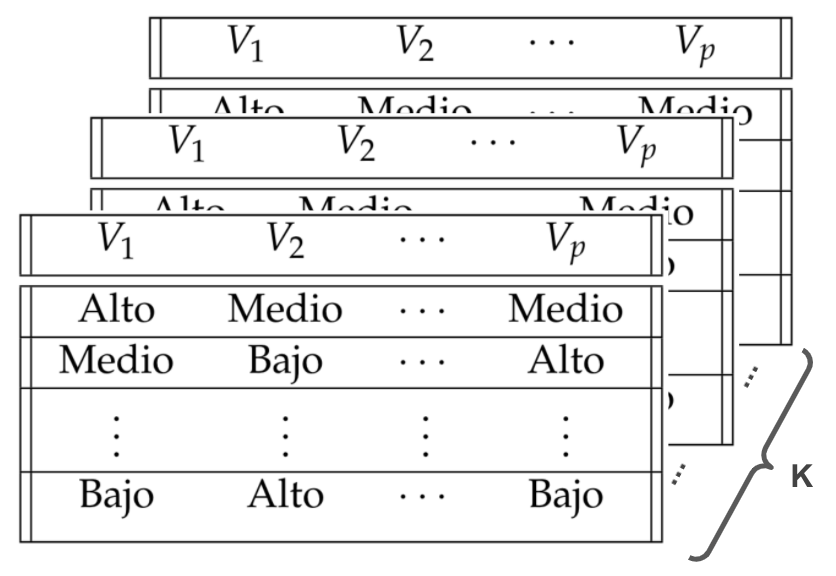
\includegraphics[width=0.4\linewidth,]{ktables} \end{center}

\caption{$k$ tablas con el formato inicial.}

\label{fig:ktables}
\end{figure}

La generalización a \emph{k} tablas del procedimiento del MCA, se
presenta en la Figura \ref{fig:MCAk}

\begin{figure}[!h]


\begin{center}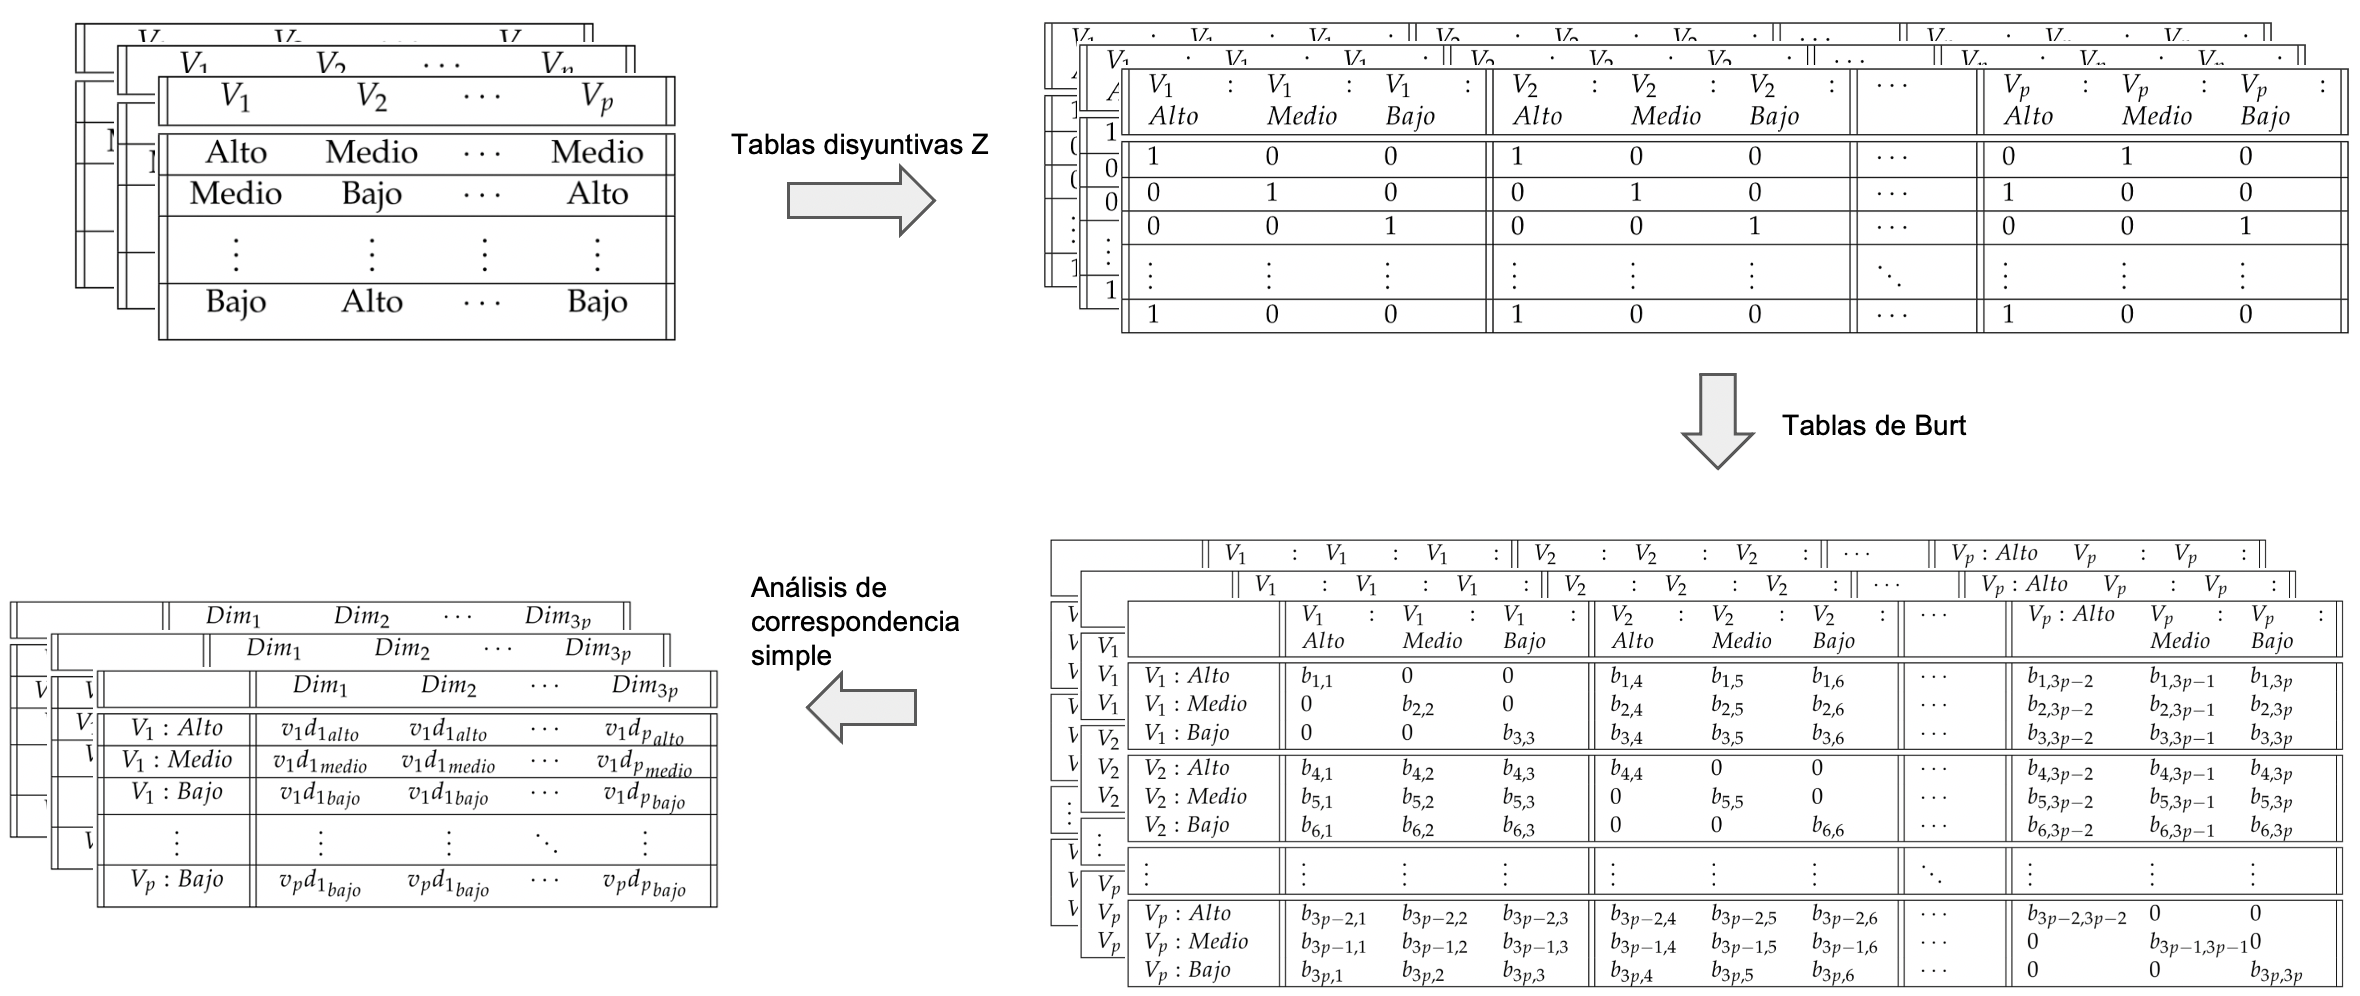
\includegraphics[width=0.9\linewidth,]{ktablesMCA} \end{center}

\caption{Procedimiento del MCA para $k$ tablas}

\label{fig:MCAk}
\end{figure}

Se llama \(C\) a cada tabla de coordenadas. Con la finalidad de detectar
la magnitud de las variables latentes, su aporte neto a las variables,
se trata la matriz \(C\) con valor absoluto.\\
Hasta este punto se tiene un conjunto de matrices de coordenadas, cuyas
filas contienen las variables observadas y las columnas, las variables
latentes.

\hypertarget{normalizaciuxf3n-de-tablas}{%
\subsubsection{Normalización de
tablas}\label{normalizaciuxf3n-de-tablas}}

Una vez que se tienen las coordenadas de las columnas, se procede a
realizar la normalización, característica del procedimiento
\emph{Análisis factorial múltiple (MFA)}.

Sea \(\lambda_{1}^{k}\) el primer valor propio obtenido de la
descomposición singular de la k-ésima tabla C. Se normaliza la tabla
multiplicándola por \(1/\lambda_{1}^{k}\). Con esto se obtiene la tabla
\(C^{'}\), que corresponde a la tabla de coordenadas normalizadas.\\
Individualmente, para el caso de la matriz k, se tendría la siguiente
expresión.

\begin{equation}
\mathbf{C'_k}=\frac{1}{\lambda_{k}^1} \mathbf{C_k}
\label{eq:Cprimak}
\end{equation}

La expresión de la ecuación \ref{eq:Cprimak} aplicada a k tablas se
representa en la figura \ref{fig:esquema1}, que muestra el esquema de
preparación de las tablas, previo a la obtención de vectores de
centralidad usados por el gráfico de control multivariante.\\
Hasta este punto se tiene un conjunto de matrices de coordenadas
normalizadas, cuyas filas contienen las variables observadas y las
columnas, las variables latentes.

\begin{figure}[!h]


\begin{center}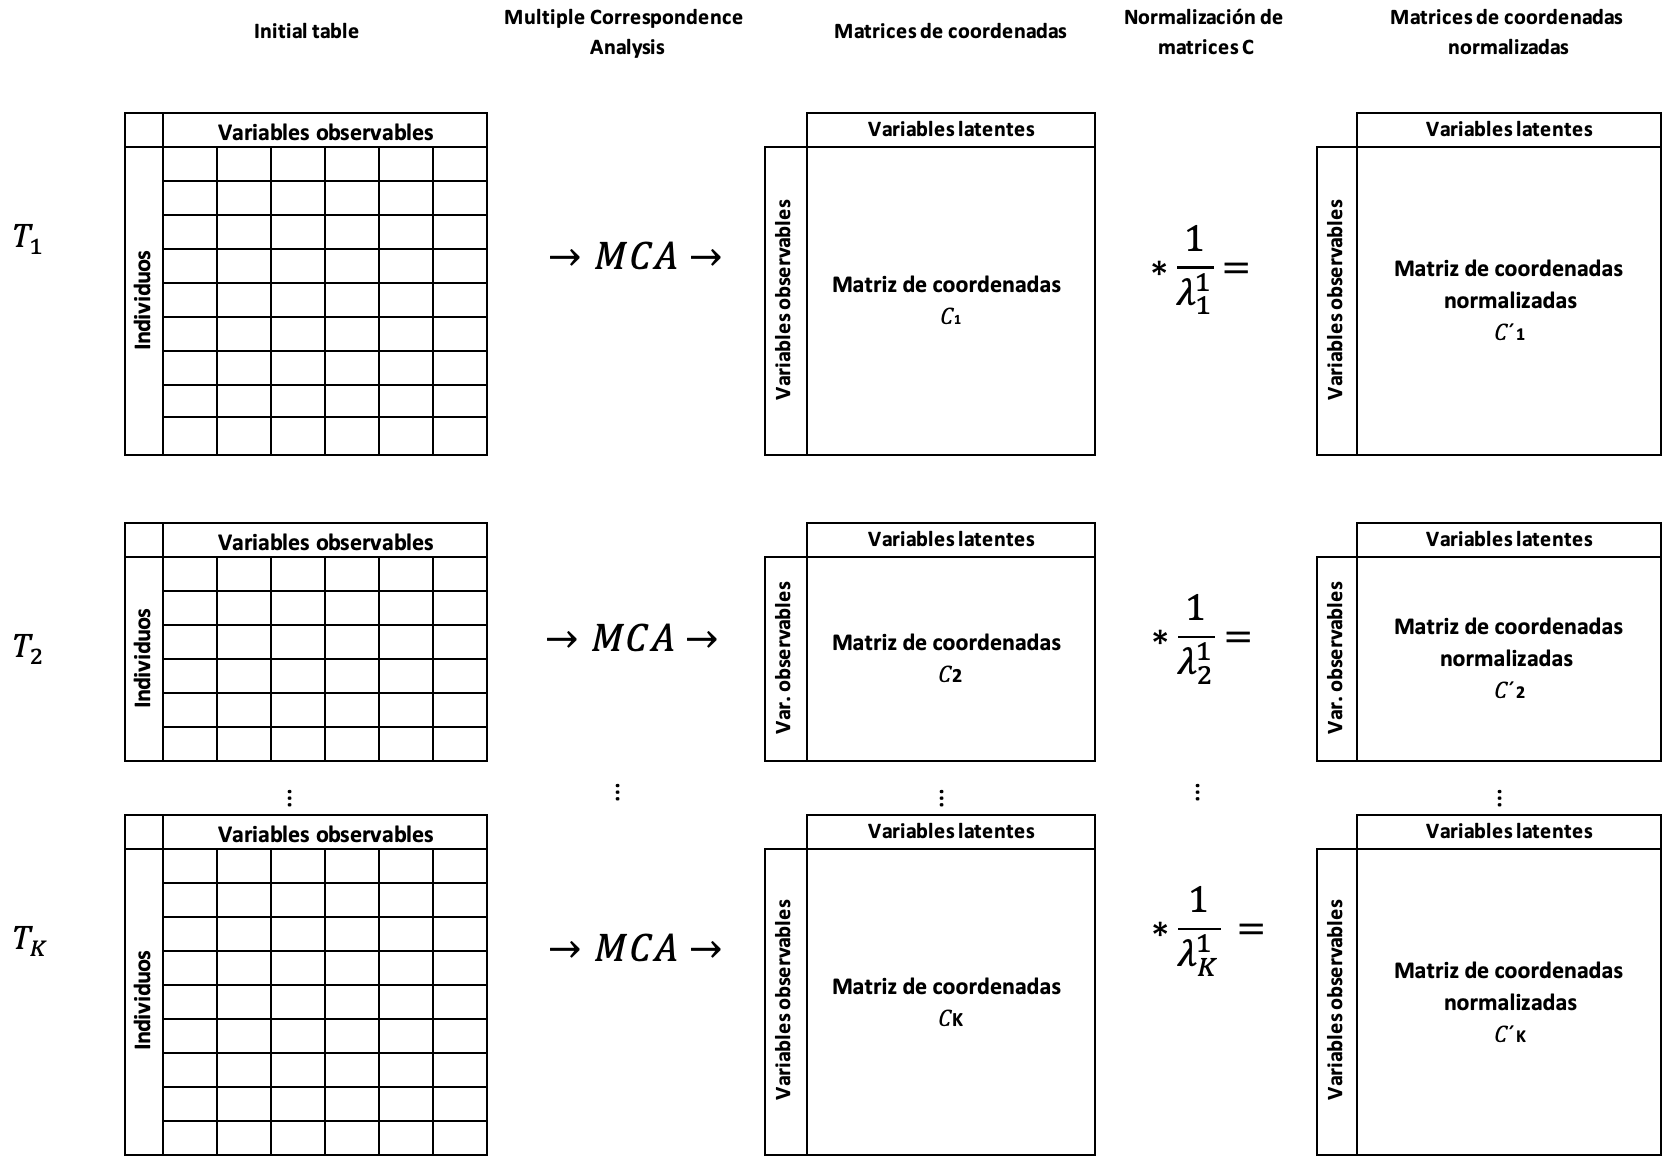
\includegraphics[width=0.9\linewidth,]{esquema_1} \end{center}

\caption{Esquema de preparación de las k tablas.}

\label{fig:esquema1}
\end{figure}

Aglomerando las matrices normalizadas \(C^{'}\) en una sola, se tiene la
matriz \(\mathbb{C}^{'}\), denominada Matriz Concatenada. Esta contiene
todos los elementos de las \emph{k} tablas normalizadas.

\begin{equation}
\mathbf{\mathbb{C^{'}}}=[\mathbf{C_1^{'}}|\mathbf{C_2^{'}}|,...,|\mathbf{C'_{K}}]^{T}
\label{eq:Cprima}
\end{equation}

La normalización que realiza el MFA se encarga de ponderar las \emph{k}
tablas, con el objetivo de evitar alguna descompensación al momento de
realizar el análisis conjunto de las tablas.

Una vez que se tiene las matrices \(\mathbf{\mathbb{C^{'}}}\) y
\(\mathbf{C_k^{'}}\), se procede a obtener los vectores de mediana, tal
como se muestra en la figura \ref{fig:esquema2}. El vector
\(\mathbf{\tilde{x}_{C_k^{'}}}\) explicará el comportamiento central de
la tabla k y el vector \(\mathbf{\tilde{x}_{\mathbb{C^{'}}}}\) explicará
el comportamiento de la matriz concatenada.

\begin{figure}[!h]


\begin{center}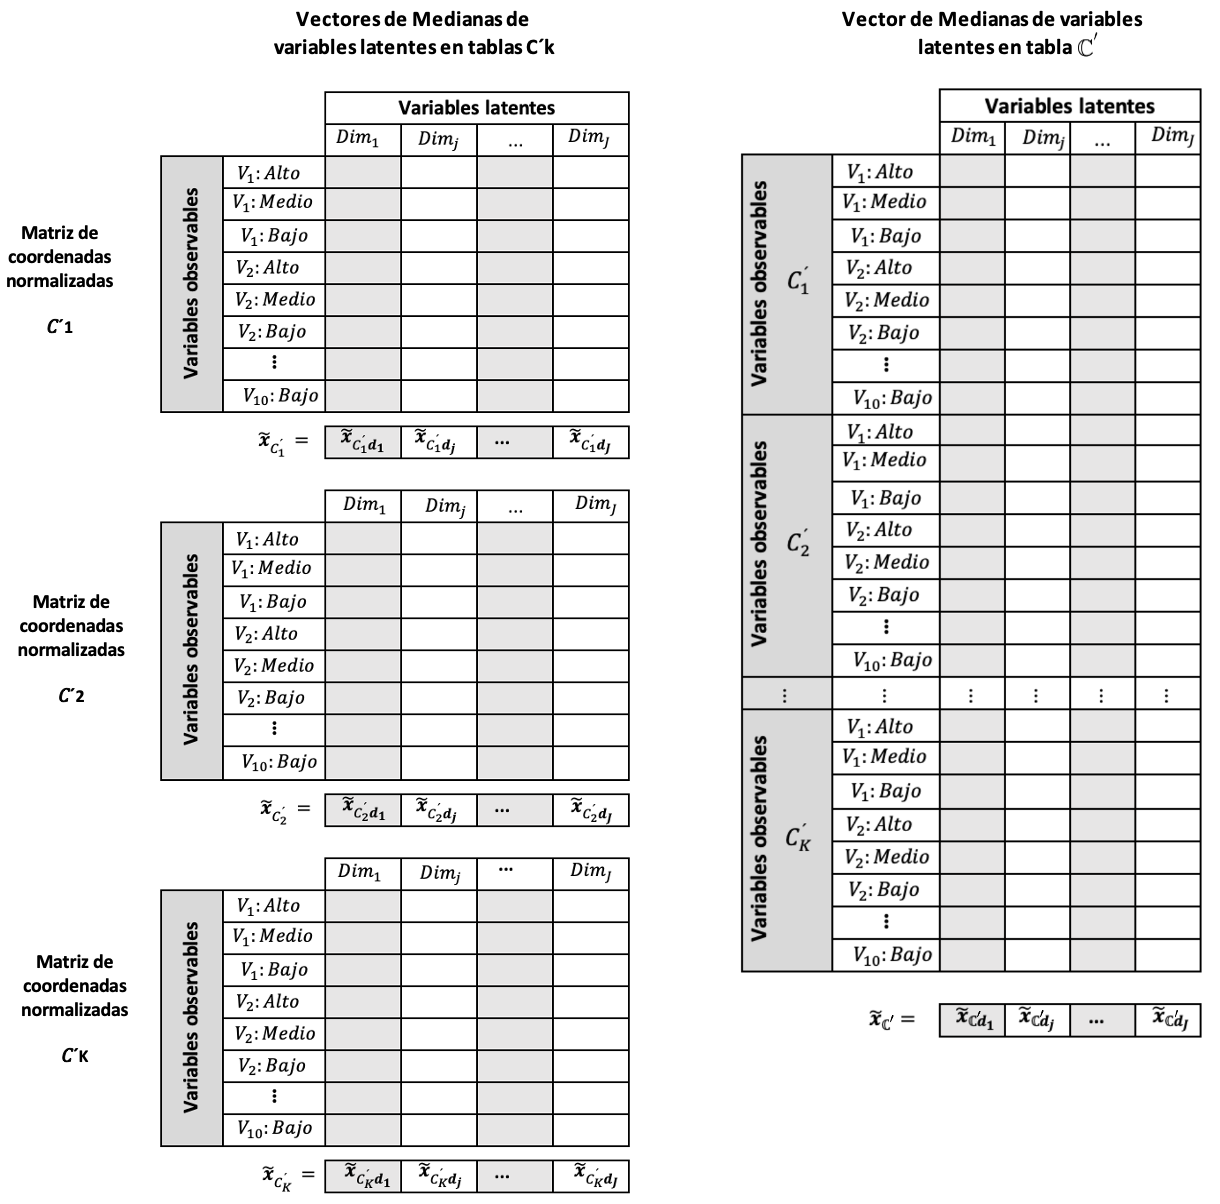
\includegraphics[width=0.9\linewidth,]{esquema_2} \end{center}

\caption{Esquema de obtención de vectores de medianas}

\label{fig:esquema2}
\end{figure}

\hypertarget{gruxe1fico-de-control-t2qv}{%
\subsection{Gráfico de control T2Qv}\label{gruxe1fico-de-control-t2qv}}

\hypertarget{obtenciuxf3n-del-gruxe1fico-de-control}{%
\subsubsection{Obtención del gráfico de
control}\label{obtenciuxf3n-del-gruxe1fico-de-control}}

Para definir el gráfico de control \(T^2\) Hotelling se deben tomar las
siguientes consideraciones:

\begin{itemize}
\tightlist
\item
  La tabla \(\mathbb{C}^{'}\) (Ecuación \ref{eq:Cprima}) se denomina
  Concatenada, sirve como referente para el escenario \emph{bajo
  control}.
\item
  El estadístico \(T^2\) Hotelling normalmente se calcula con los
  vectores de media y considera la variabilidad de todas las tablas,
  incluyendo las que estén potencialmente contaminadas, es decir, las
  que se representarían como puntos fuera de control en el gráfico T2Qv.
  Esto puede generar un problema, dado que, en esta fase I se espera que
  la matriz concatenada capture el comportamiento ``en control''. Para
  resolver este inconveniente se suele excluir del análisis a las tablas
  que difieren del comportamiento normal, sin embargo, la propuesta de
  esta investigación es adoptar conceptos de robustez, utilizando el
  vector de medianas en vez de el de medias, en virtud de que a las
  medianas no les afectan los valores atípicos.
\item
  De la matriz concatenada \(\mathbb{C}^{'}\) se obtiene
  \(\tilde{x_{0}}\) (Vector de medianas de la matriz concatenada) y
  \(S_0\) (Matriz de covarianzas de la matriz concatenada).
\item
  Cada matriz \(\mathbf{C'_k}\) tiene el mismo número de columnas (p)
  (variables).
\item
  El vector de medias \(\tilde{x_{k}}\) está atado a la tabla
  \(\mathbf{C'_k}\), es decir, el gráfico de control estará en función
  de las diferencias entre las matrices \(\mathbf{C'_k}\) y la matriz
  concatenada \(\mathbf{\mathbb{C^{'}}}\).
\item
  Las matrices \(\mathbf{C'_k}\) siguen una distribución normal
  multivariante con vector de centralidad \(\tilde{x_{k}}\) y matriz de
  covarianzas \(\mathbf{S_k}\).
\end{itemize}

El estadístico \(T^2\) viene dado por:

\begin{equation}
T^2=n (\mu_{k}-\mu_{0})'\mathbf{\Sigma_{0}^{-1}}(\mu_{k}-\mu_{0})
\label{eq:T2}
\end{equation}

Tomando en cuenta las consideraciones previas, se obtiene el estadístico
\(T^2_{med}\)

\begin{equation}
T^2_{med}=n (\tilde{x_{k}}-\tilde{x_{0}})'\mathbf{\Sigma_{0}^{-1}}(\tilde{x_{k}}-\tilde{x_{0}})
\label{eq:T2med}
\end{equation}

Se sabe que, bajo control, el \(T^2\) se distribuye como una
Chi-cuadrado con \(p\) grados de libertad \(\chi^2_p\). En este caso se
puede aplicar este principio, ya que se utiliza la matriz concatenada
(\(\mathbb{C}^{'}\)), que representa al escenario bajo control.

Dado que este gráfico de control está basado en distancias de
Mahalanobis ponderadas, sólo tiene límite de control superior. Este
viene dado por la ecuación \ref{eq:UCL}

\begin{equation}
UCL=\chi^2_{\alpha,p}
\label{eq:UCL}
\end{equation}

donde \(p\) es el número de dimensiones y \(\alpha\) es la significancia
predeterminada, se considera \(\alpha=0.0027\).

\hypertarget{interpretaciuxf3n-de-puntos-fuera-de-control}{%
\subsubsection{Interpretación de puntos fuera de
control}\label{interpretaciuxf3n-de-puntos-fuera-de-control}}

El gráfico multivariante \(T^2\) de Hotelling para variables
cualitativas es capaz de señalar que el proceso salió de control, pero
no permite reconocer el momento ni las causas por las que ocurrió esto.
Es obvio que, más allá de reconocer el estado del proceso, interesa
saber cuándo y por qué salió de control. Es importante tener en cuenta
que cada punto representado en el gráfico \(T^2\) de Hotelling
representa a una tabla (muestra), constituida por un grupo de individuos
(observaciones) y \emph{p} variables que pueden tener muchas categorías,
algunas de éstas pueden mostrar un comportamiento anómalo. Por
consiguiente, es necesario analizar con detenimiento que está pasando
con los datos de las tablas reportadas.

Este análisis se realiza comparando la ubicación de los puntos que
representan las categorías de las variables en el MCA de la tabla
concatenada y la ubicación de los puntos en los gráficos MCA de cada
tabla reportada como fuera de control. Las categorías que están
incidiendo en el estado fuera de control son aquellas cuya ubicación en
ambas tablas comparadas muestra diferencias importantes. Para
cuantificar la magnitud del comportamiento anómalo de estas categorías
se calcula las distancias Chi-cuadrado entre las masas de las columnas
de la tabla reportada como fuera de control y las de la tabla
concatenada, tomada como referente. Mientras mayor es el valor del
estadístico, mayor es su incidencia en el desplazamiento de la
centralidad del proceso que, finalmente, pueden llevarlo a un estado
fuera de control.

\hypertarget{gruxe1fico-de-diferencias-chi-cuadrado}{%
\subsection{Gráfico de diferencias Chi
Cuadrado}\label{gruxe1fico-de-diferencias-chi-cuadrado}}

Consiste en un gráfico interactivo de barras que representa a las
distancias \(\chi^2\) entre las masas de columna de las variables de la
tabla concatenada y la tabla \emph{i}, que podría ser la que está fuera
de control u otra que se quisiera analizar. Las barras que denotan mayor
altura son las que más están incidiendo en la variación de la tendencia
central del proceso y, por consiguiente, su salida de control. Para
proporcionar mayor detalle, este gráfico interactivo también ofrece,
mediante un gráfico circular anidado, una representación de la
distribución de las categorías de la variable observada, correspondiente
a la tabla \emph{i}, así como un gráfico circular de la distribución de
las categorías de la tabla concatenada.\\
De esta manera, la metodología propuesta en esta investigación permite
explicar cuándo y por qué el proceso salió de control.

\hypertarget{complemento-computacional}{%
\section{Complemento computacional}\label{complemento-computacional}}

Para facilitar la difusión y aplicación del método propuesto, se ha
desarrollado un paquete reproducible en R. El paquete \textbf{T2Qv}
\citep{T2Qv} realiza el análisis de control de \emph{k} tablas por medio
de gráficos de control multivariantes para variables cualitativas,
utilizando los fundamentos del análisis de correspondencias múltiples y
el análisis factorial múltiple. Los gráficos se pueden mostrar de forma
plana o interactiva, de la misma manera todas las salidas se pueden
mostrar en un panel interactivo de Shiny.

\hypertarget{disponibilidad}{%
\subsection{Disponibilidad}\label{disponibilidad}}

El paquete está disponible en el repositorio oficial de R, The
Comprehensive R Archive Network (CRAN), la descarga se la puede realizar
de la siguiente forma:

\begin{verbatim}
install.packages("T2Qv")
\end{verbatim}

\hypertarget{el-paquete-t2qv}{%
\subsection{El paquete: T2Qv}\label{el-paquete-t2qv}}

\begin{figure}[!ht]



\begin{center}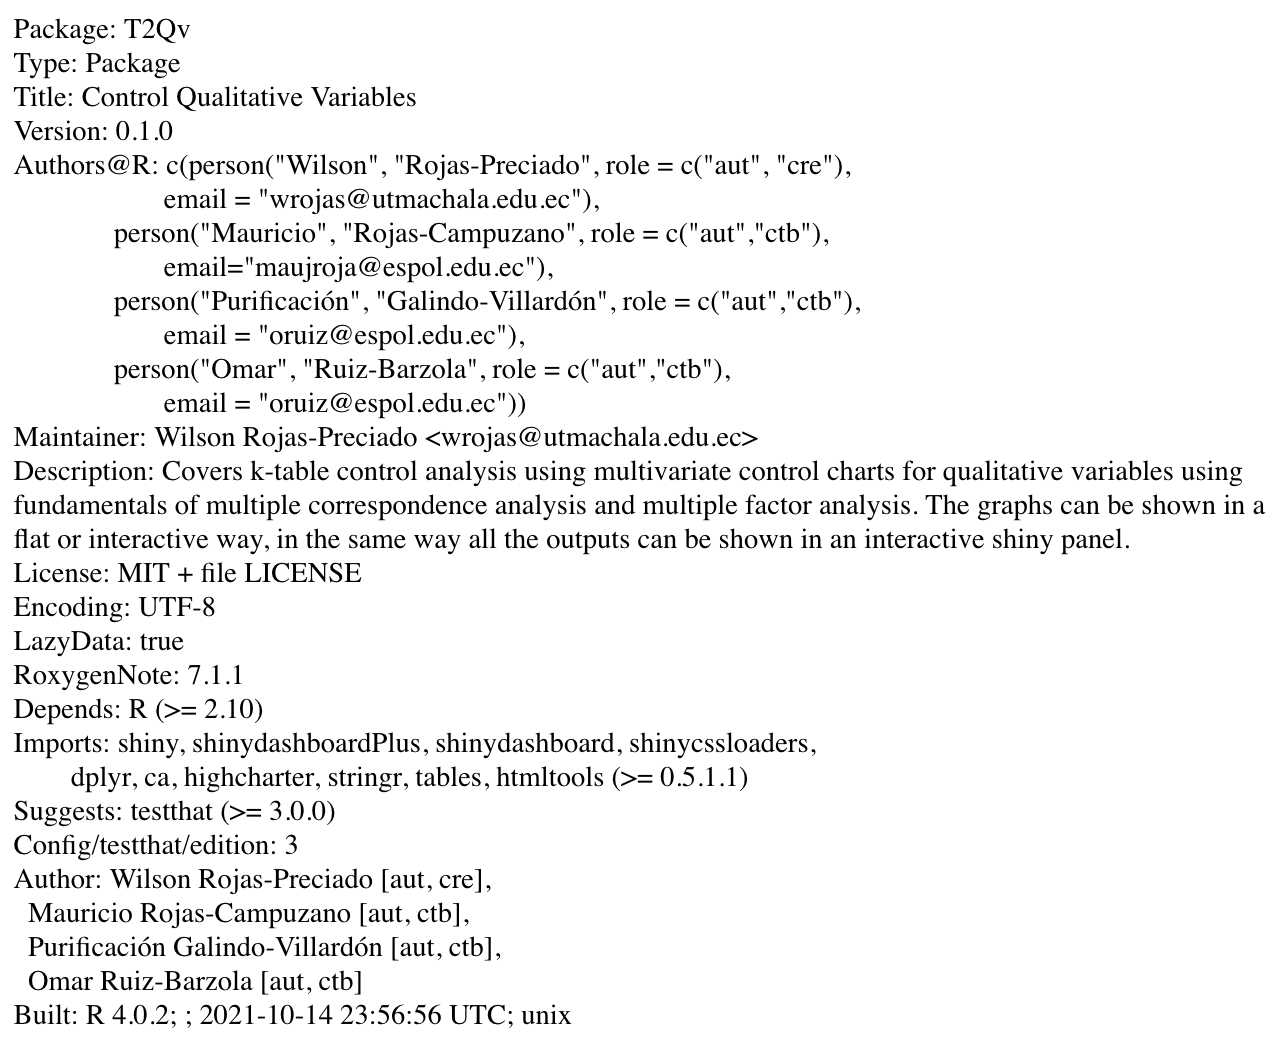
\includegraphics[width=0.6\linewidth,]{DescrPack} \end{center}

\caption{Documentación del paquete T2Qv}

\label{fig:documentation}
\end{figure}

Las funciones que contiene el paquete y su descripción se enuncian en la
tabla \ref{tab:functions}.

\begin{table}[h!]
\begin{center}
 \begin{tabular}{||c  m{35em}||} 
 \hline
  Función & Descripción \\ [0.5ex] 
 \hline\hline
 T2 qualitative & Multivariate control chart T2 Hotelling applicable for qualitative variables.\\
 \hline
  MCAconcatenated & Multiple correspondence analysis applied to a concatenated table.\\
\hline
  MCApoint & Multiple correspondence analysis applied to a specific table.\\
\hline
  ChiSq variable & Contains Chi square distance between the column masses of the table specified in PointTable and the concatenated table. It allows to identify which mode is responsible for the anomaly in the table in which it is located. \\ [1ex] 
  \hline
  Full Panel & A shiny panel complete with the 
  multivariate control chart for 
  qualitative variables, the two MCA 
  charts and the modality distance table. 
  Within the dashboard, arguments such as 
  type I error and dimensionality can be 
  modified. \\ [1ex] 
 \hline
\end{tabular}\caption{Funciones del paquete T2Qv}
\label{tab:functions}
\end{center}
\end{table}

2022-2023 \# Resultados

Con la intención de probar la metodología propuesta en el gráfico de
control \(T^2\) de Hotelling para variables cualitativas, se hizo un
análisis con datos simulados y otro con datos reales aplicados al
contexto de la educación superior. Los resultados se obtienen de la
aplicación del paquete T2Qv.

\hypertarget{resultados-con-datos-simulados}{%
\subsection{Resultados con datos
simulados}\label{resultados-con-datos-simulados}}

\hypertarget{generaciuxf3n-de-datos-simulados}{%
\subsubsection{Generación de datos
simulados}\label{generaciuxf3n-de-datos-simulados}}

\label{simulados}

Para este estudio se generó una base de datos simulados, a la que se
denominó \emph{Datak10Contaminated}. Consta de 10 tablas, cada una de
ellas está constituida por 100 filas (observaciones) y 11 columnas, de
las cuales, las 10 primeras corresponden a las variables analizadas (V1,
V2, \ldots; V10), mismas que contienen 3 categorías (Alto, Medio y
Bajo), mientras que, la columna 11, denominada \emph{GroupLetter},
contiene el factor de clasificación de los grupos. Para su
identificación, las tablas han sido denominadas con las letras del
alfabeto, desde la \emph{a} hasta la \emph{j}. La tabla \emph{j} tiene
una distribución distinta de la que tienen las otras nueve. Las 9
primeras tablas tienen sus 10 variables con la siguiente distribución:

\[ u \sim U[0,1]\]

\[t_{1,..,9}= \left\{ \begin{array}{lcc}
             Bajo &   si  & u \leq 1/3 \\
             \\ Medio &  si & 1/3 < u < 2/3 \\
             \\ Alto &  si  & u \geq 2/3 
             \end{array}
   \right. \]

La tabla 10, en todas sus 10 variables, sigue la distribución presentada
a continuación:

\[ u \sim U[0,1]\]

\[t_{10}= \left\{ \begin{array}{lcc}
             Bajo &   si  & u \leq 1/5 \\
             \\ Medio &  si & 1/5 < u < 2/6 \\
             \\ Alto &  si  & u \geq 2/6 
             \end{array}
   \right. \]

La base de datos se presenta en el formato establecido en la tabla
\ref{tab:tabladatos}.

\begin{table}[!ht]
\tiny
\centering
\resizebox{13cm}{!} {
\begin{tabular}{@{}lllllllllll@{}}
\toprule
\textbf{V1}                  & \textbf{V2}                    & \textbf{V3}                  & \textbf{V4}                    & \textbf{V5}                  & \textbf{V6}                    & \textbf{V7}                    & \textbf{V8}                    & \textbf{V9}                    & \textbf{V10}                   & \textbf{GroupLetter}      \\ \midrule
Low      & Medium     & Medium                       & High                           & High                         & High                           & Low                            & Medium                         & Medium                         & Medium                         & a                         \\
Low                          & Low                            & High                         & Low                            & Medium                       & High                           & High                           & High                           & Low                            & High                           & a \\
High & Medium & High & Low    & High & Medium & Medium & High   & Medium & Low    & a                         \\
Medium                       & Medium                         & Low                          & High                           & Low                          & Medium                         & High                           & Low                            & Low                            & High                           & a \\
Low  & Low    & Low  & High   & Low  & High   & High   & High   & Medium & Medium & a                         \\
High                         & High                           & Medium                       & Low                            & High                         & Low                            & Medium                         & Medium                         & High                           & Low                            & a \\
High & High   & Low  & Low    & Low  & Medium & High   & Medium & Medium & High   & a                         \\
Medium                       & Medium                         & High                         & Medium                         & Medium                       & High                           & Medium                         & High                           & High                           & High                           & a \\
Low  & Low    & Low  & Medium & High & Medium & Low    & Medium & Low    & Low    & a                         \\
Medium                       & Medium                         & Medium                       & High                           & Low                          & Medium                         & High                           & Low                            & High                           & Medium                         & a \\ \bottomrule
\end{tabular}
}

\caption{Sección de la base de datos $Datak10Contaminated$.}

\label{tab:tabladatos}

\end{table}

Para verificar la diferencia entre las distribuciones de la tabla 10 y
las demás, se calculó el promedio de las frecuencias relativas en las
tres categorías, desde la tabla \emph{a} hasta la \emph{i}, para las 10
variables (Tabla \ref{tab:tablan}), luego se calculó el promedio de las
frecuencias relativas medias de las 10 variables, el resultado permite
comparar la distribución de las categorías de la tabla
\emph{Datak10Contaminated} con la distribución teórica uniforme, como se
observa en la tabla \ref{tab:tablapromfreq}.

\begin{table}[H]
\centering
\begin{tabular}{@{}clrrrrrrrrrr@{}}
\toprule
\textbf{Tabla} & \textbf{Categoría} & \multicolumn{1}{l}{\textbf{V1}} & \multicolumn{1}{l}{\textbf{V2}} & \multicolumn{1}{l}{\textbf{V3}} & \multicolumn{1}{l}{\textbf{V4}} & \multicolumn{1}{l}{\textbf{V5}} & \multicolumn{1}{l}{\textbf{V6}} & \multicolumn{1}{l}{\textbf{V7}} & \multicolumn{1}{l}{\textbf{V8}} & \multicolumn{1}{l}{\textbf{V9}} & \multicolumn{1}{l}{\textbf{V10}} \\ \midrule
\rowcolor[HTML]{D9D9D9} 
\textbf{a}     & \textbf{High}      & 0.29                               & 0.25                               & 0.36                               & 0.38                               & 0.38                               & 0.35                               & 0.36                               & 0.29                               & 0.33                               & 0.37                                \\
\rowcolor[HTML]{D9D9D9} 
\textbf{a}     & \textbf{Medium}    & 0.36                               & 0.49                               & 0.34                               & 0.34                               & 0.31                               & 0.41                               & 0.38                               & 0.28                               & 0.38                               & 0.31                                \\
\rowcolor[HTML]{D9D9D9} 
\textbf{a}     & \textbf{Low}       & 0.35                               & 0.26                               & 0.30                               & 0.28                               & 0.31                               & 0.24                               & 0.26                               & 0.43                               & 0.29                               & 0.32                                \\
\textbf{b}     & \textbf{High}      & 0.31                               & 0.44                               & 0.37                               & 0.29                               & 0.31                               & 0.34                               & 0.30                               & 0.36                               & 0.29                               & 0.34                                \\
\textbf{b}     & \textbf{Medium}    & 0.40                               & 0.31                               & 0.30                               & 0.35                               & 0.37                               & 0.32                               & 0.35                               & 0.30                               & 0.39                               & 0.36                                \\
\textbf{b}     & \textbf{Low}       & 0.29                               & 0.25                               & 0.33                               & 0.36                               & 0.32                               & 0.34                               & 0.35                               & 0.34                               & 0.32                               & 0.30                                \\
\rowcolor[HTML]{D9D9D9} 
\textbf{c}     & \textbf{High}      & 0.34                               & 0.33                               & 0.25                               & 0.35                               & 0.32                               & 0.30                               & 0.39                               & 0.40                               & 0.41                               & 0.43                                \\
\rowcolor[HTML]{D9D9D9} 
\textbf{c}     & \textbf{Medium}    & 0.36                               & 0.33                               & 0.25                               & 0.32                               & 0.32                               & 0.32                               & 0.27                               & 0.35                               & 0.32                               & 0.35                                \\
\rowcolor[HTML]{D9D9D9} 
\textbf{c}     & \textbf{Low}       & 0.30                               & 0.34                               & 0.50                               & 0.33                               & 0.36                               & 0.38                               & 0.34                               & 0.25                               & 0.27                               & 0.22                                \\
\textbf{d}     & \textbf{High}      & 0.32                               & 0.34                               & 0.34                               & 0.38                               & 0.41                               & 0.33                               & 0.35                               & 0.46                               & 0.34                               & 0.45                                \\
\textbf{d}     & \textbf{Medium}    & 0.35                               & 0.30                               & 0.28                               & 0.31                               & 0.27                               & 0.35                               & 0.30                               & 0.24                               & 0.33                               & 0.24                                \\
\textbf{d}     & \textbf{Low}       & 0.33                               & 0.36                               & 0.38                               & 0.31                               & 0.32                               & 0.32                               & 0.35                               & 0.30                               & 0.33                               & 0.31                                \\
\rowcolor[HTML]{D9D9D9} 
\textbf{e}     & \textbf{High}      & 0.32                               & 0.32                               & 0.36                               & 0.26                               & 0.36                               & 0.31                               & 0.29                               & 0.28                               & 0.32                               & 0.41                                \\
\rowcolor[HTML]{D9D9D9} 
\textbf{e}     & \textbf{Medium}    & 0.34                               & 0.40                               & 0.34                               & 0.40                               & 0.38                               & 0.37                               & 0.27                               & 0.37                               & 0.32                               & 0.23                                \\
\rowcolor[HTML]{D9D9D9} 
\textbf{e}     & \textbf{Low}       & 0.34                               & 0.28                               & 0.30                               & 0.34                               & 0.26                               & 0.32                               & 0.44                               & 0.35                               & 0.36                               & 0.36                                \\
\textbf{f}     & \textbf{High}      & 0.31                               & 0.29                               & 0.27                               & 0.32                               & 0.36                               & 0.32                               & 0.26                               & 0.41                               & 0.34                               & 0.26                                \\
\textbf{f}     & \textbf{Medium}    & 0.41                               & 0.29                               & 0.36                               & 0.31                               & 0.31                               & 0.38                               & 0.36                               & 0.33                               & 0.30                               & 0.37                                \\
\textbf{f}     & \textbf{Low}       & 0.28                               & 0.42                               & 0.37                               & 0.37                               & 0.33                               & 0.30                               & 0.38                               & 0.26                               & 0.36                               & 0.37                                \\
\rowcolor[HTML]{D9D9D9} 
\textbf{g}     & \textbf{High}      & 0.27                               & 0.39                               & 0.34                               & 0.38                               & 0.28                               & 0.31                               & 0.35                               & 0.38                               & 0.27                               & 0.34                                \\
\rowcolor[HTML]{D9D9D9} 
\textbf{g}     & \textbf{Medium}    & 0.42                               & 0.27                               & 0.32                               & 0.35                               & 0.37                               & 0.32                               & 0.35                               & 0.36                               & 0.41                               & 0.26                                \\
\rowcolor[HTML]{D9D9D9} 
\textbf{g}     & \textbf{Low}       & 0.31                               & 0.34                               & 0.34                               & 0.27                               & 0.35                               & 0.37                               & 0.30                               & 0.26                               & 0.32                               & 0.40                                \\
\textbf{h}     & \textbf{High}      & 0.32                               & 0.47                               & 0.34                               & 0.38                               & 0.47                               & 0.34                               & 0.32                               & 0.35                               & 0.35                               & 0.31                                \\
\textbf{h}     & \textbf{Medium}    & 0.28                               & 0.31                               & 0.29                               & 0.27                               & 0.27                               & 0.43                               & 0.39                               & 0.35                               & 0.36                               & 0.40                                \\
\textbf{h}     & \textbf{Low}       & 0.40                               & 0.22                               & 0.37                               & 0.35                               & 0.26                               & 0.23                               & 0.29                               & 0.30                               & 0.29                               & 0.29                                \\
\rowcolor[HTML]{D9D9D9} 
\textbf{i}     & \textbf{High}      & 0.32                               & 0.42                               & 0.29                               & 0.30                               & 0.26                               & 0.28                               & 0.38                               & 0.38                               & 0.36                               & 0.36                                \\
\rowcolor[HTML]{D9D9D9} 
\textbf{i}     & \textbf{Medium}    & 0.35                               & 0.34                               & 0.29                               & 0.33                               & 0.47                               & 0.38                               & 0.25                               & 0.29                               & 0.33                               & 0.31                                \\
\rowcolor[HTML]{D9D9D9} 
\textbf{i}     & \textbf{Low}       & 0.33                               & 0.24                               & 0.42                               & 0.37                               & 0.27                               & 0.34                               & 0.37                               & 0.33                               & 0.31                               & 0.33                                \\
\textbf{j}     & \textbf{High}      & 0.75                               & 0.71                               & 0.78                               & 0.71                               & 0.70                               & 0.73                               & 0.69                               & 0.66                               & 0.73                               & 0.78                                \\
\textbf{j}     & \textbf{Medium}    & 0.08                               & 0.10                               & 0.01                               & 0.06                               & 0.10                               & 0.12                               & 0.11                               & 0.12                               & 0.12                               & 0.10                                \\
\textbf{j}     & \textbf{Low}       & 0.17                               & 0.19                               & 0.21                               & 0.23                               & 0.20                               & 0.15                               & 0.20                               & 0.22                               & 0.15                               & 0.12                                \\
\rowcolor[HTML]{D9D9D9} 
$\bar{x}_{a, b, ...,  i}$        & \textbf{High}      & \textbf{0.31}                      & \textbf{0.37}                      & \textbf{0.33}                      & \textbf{0.33}                      & \textbf{0.35}                      & \textbf{0.32}                      & \textbf{0.33}                      & \textbf{0.37}                      & \textbf{0.33}                      & \textbf{0.36}                       \\
\rowcolor[HTML]{D9D9D9} 
$\bar{x}_{a, b, ...,  i}$          & \textbf{Medium}    & \textbf{0.37}                      & \textbf{0.34}                      & \textbf{0.31}                      & \textbf{0.33}                      & \textbf{0.34}                      & \textbf{0.36}                      & \textbf{0.33}                      & \textbf{0.32}                      & \textbf{0.35}                      & \textbf{0.32}                       \\
\rowcolor[HTML]{D9D9D9} 
$\bar{x}_{a, b, ...,  i}$           & \textbf{Low}       & \textbf{0.32}                      & \textbf{0.30}                      & \textbf{0.36}                      & \textbf{0.33}                      & \textbf{0.31}                      & \textbf{0.32}                      & \textbf{0.34}                      & \textbf{0.32}                      & \textbf{0.32}                      & \textbf{0.32}                       \\ \bottomrule
\end{tabular}
\caption{Promedio de frecuencias relativas medias en las tres categorías, desde la tabla $a$ hasta la $i$. $Data10Contaminated$}

\label{tab:tablan}
\end{table}

\begin{table}[H]
\centering
\begin{tabular}{rccc}
\hline
\toprule

\textbf{Categorías} & \textbf{Teórica uniforme} & \textbf{Promedio Tablas $a$, $b$, ...,  $i$} & \textbf{Promedio Tabla $j$} \\ \midrule
\textbf{High}       & 0.333            & 0.340                & 0.724            \\ 
\textbf{Medium}     & 0.333            & 0.336                & 0.092            \\ 
\textbf{Low}        & 0.333            & 0.324                & 0.184            \\ \midrule
\end{tabular}
\caption{Comparación de la distribución de las categorías de la tabla $Datak10Contaminated$ con la distribución teórica uniforme.}
\label{tab:tablapromfreq}
\end{table}

Con estos datos se aplicaron pruebas Chi cuadrado de bondad de ajuste.
Las hipótesis nulas consideran que la distribución de las categorías de
la tabla \emph{j} es igual que la distribución de cada una de las demás
tablas (uniforme Low 0.333, Medium 0.333 y High 0.333). Se encontró, con
un nivel de confianza del 95\%, que las distribuciones de todas las
variables de la tabla \emph{j} mostraron diferencias estadísticamente
significativas con las distribuciones de las variables de las demás
tablas, con 2 grados de libertad. La tabla \ref{tab:tablapromfreqsumm}
presenta el resumen de los estadísticos de prueba respectivos. Como
conclusión se ratifica que la tabla \emph{j} tiene una distribución
diferente de todas las demás tablas.

\begin{table}[H]
\centering
\begin{tabular}{llrrrrrrrrrr}
\toprule
\multicolumn{1}{c}{\textbf{GroupLetter}} & \multicolumn{1}{c}{\textbf{Estadísticos}} & \multicolumn{1}{c}{\textbf{V1}}      & \multicolumn{1}{c}{\textbf{V2}}      & \multicolumn{1}{c}{\textbf{V3}}      & \multicolumn{1}{c}{\textbf{V4}}      & \multicolumn{1}{c}{\textbf{V5}}      & \multicolumn{1}{c}{\textbf{V6}}      & \multicolumn{1}{c}{\textbf{V7}}      & \multicolumn{1}{c}{\textbf{V8}}      & \multicolumn{1}{c}{\textbf{V9}}      & \multicolumn{1}{c}{\textbf{V10}}     \\ \midrule

                                           & Chi-cuadrado                               & 0.86                                  & 11.06                                 & 0.56                                  & 1.52                                  & 0.98                                  & 4.46                                  & 2.48                                  & 4.22                                  & 1.22                                  & 0.62                                  \\ \cline{2-12} 
\multirow{-2}{*}{\textbf{a}}               & \textit{p-valor}                           & \textit{0.651}                        & {\color[HTML]{C00000} \textit{0.004}} & \textit{0.756}                        & \textit{0.468}                        & \textit{0.613}                        & \textit{0.108}                        & \textit{0.289}                        & \textit{0.121}                        & \textit{0.543}                        & \textit{0.733}                        \\ \hline
                                           & Chi-cuadrado                               & 2.06                                  & 5.66                                  & 0.74                                  & 0.86                                  & 0.62                                  & 0.08                                  & 0.50                                  & 0.56                                  & 1.58                                  & 0.56                                  \\ \cline{2-12} 
\multirow{-2}{*}{\textbf{b}}               & p-valor                                    & \textit{0.357}                        & \textit{0.059}                        & \textit{0.691}                        & \textit{0.651}                        & \textit{0.733}                        & \textit{0.961}                        & \textit{0.779}                        & \textit{0.756}                        & \textit{0.454}                        & \textit{0.756}                        \\ \hline
                                           & Chi-cuadrado                               & 0.56                                  & 0.02                                  & 12.50                                 & 0.14                                  & 0.32                                  & 1.04                                  & 2.18                                  & 3.50                                  & 3.02                                  & 6.74                                  \\ \cline{2-12} 
\multirow{-2}{*}{\textbf{c}}               & \textit{p-valor}                           & \textit{0.756}                        & \textit{0.990}                        & {\color[HTML]{C00000} \textit{0.002}} & \textit{0.932}                        & \textit{0.852}                        & \textit{0.595}                        & \textit{0.336}                        & \textit{0.174}                        & \textit{0.221}                        & {\color[HTML]{C00000} \textit{0.034}} \\ \hline
                                           & Chi-cuadrado                               & 0.14                                  & 0.56                                  & 1.52                                  & 0.98                                  & 3.02                                  & 0.14                                  & 0.50                                  & 7.76                                  & 0.02                                  & 6.86                                  \\ \cline{2-12} 
\multirow{-2}{*}{\textbf{d}}               & \textit{p-valor}                           & \textit{0.932}                        & \textit{0.756}                        & \textit{0.468}                        & \textit{0.613}                        & \textit{0.221}                        & \textit{0.932}                        & \textit{0.779}                        & {\color[HTML]{C00000} \textit{0.021}} & \textit{0.990}                        & {\color[HTML]{C00000} \textit{0.032}} \\ \hline
                                           & Chi-cuadrado                               & 0.08                                  & 2.24                                  & 0.56                                  & 2.96                                  & 2.48                                  & 0.62                                  & 5.18                                  & 1.34                                  & 0.32                                  & 5.18                                  \\ \cline{2-12} 
\multirow{-2}{*}{\textbf{e}}               & \textit{p-valor}                           & \textit{0.961}                        & \textit{0.326}                        & \textit{0.756}                        & \textit{0.228}                        & \textit{0.289}                        & \textit{0.733}                        & \textit{0.075}                        & \textit{0.512}                        & \textit{0.852}                        & \textit{0.075}                        \\ \hline
                                           & Chi-cuadrado                               & 2.78                                  & 3.38                                  & 1.82                                  & 0.62                                  & 0.38                                  & 1.04                                  & 2.48                                  & 3.38                                  & 0.56                                  & 2.42                                  \\ \cline{2-12} 
\multirow{-2}{*}{\textbf{f}}               & \textit{p-valor}                           & \textit{0.249}                        & \textit{0.185}                        & \textit{0.403}                        & \textit{0.733}                        & \textit{0.827}                        & \textit{0.595}                        & \textit{0.289}                        & \textit{0.185}                        & \textit{0.756}                        & \textit{0.298}                        \\ \hline
                                           & Chi-cuadrado                               & 3.62                                  & 2.18                                  & 0.08                                  & 1.94                                  & 1.34                                  & 0.62                                  & 0.50                                  & 2.48                                  & 3.02                                  & 2.96                                  \\ \cline{2-12} 
\multirow{-2}{*}{\textbf{g}}               & \textit{p-valor}                           & \textit{0.164}                        & \textit{0.336}                        & \textit{0.961}                        & \textit{0.379}                        & \textit{0.512}                        & \textit{0.733}                        & \textit{0.779}                        & \textit{0.289}                        & \textit{0.221}                        & \textit{0.228}                        \\ \hline
                                           & Chi-cuadrado                               & 2.24                                  & 9.62                                  & 0.98                                  & 1.94                                  & 8.42                                  & 6.02                                  & 1.58                                  & 0.50                                  & 0.86                                  & 2.06                                  \\ \cline{2-12} 
\multirow{-2}{*}{\textbf{h}}               & \textit{p-valor}                           & \textit{0.326}                        & {\color[HTML]{C00000} \textit{0.008}} & \textit{0.613}                        & \textit{0.379}                        & {\color[HTML]{C00000} \textit{0.015}} & {\color[HTML]{C00000} \textit{0.049}} & \textit{0.454}                        & \textit{0.779}                        & \textit{0.651}                        & \textit{0.357}                        \\ \hline
                                           & Chi-cuadrado                               & 0.14                                  & 4.88                                  & 3.38                                  & 0.74                                  & 8.42                                  & 1.52                                  & 3.14                                  & 1.22                                  & 0.38                                  & 0.38                                  \\ \cline{2-12} 
\multirow{-2}{*}{\textbf{i}}               & \textit{p-valor}                           & \textit{0.932}                        & \textit{0.087}                        & \textit{0.185}                        & \textit{0.691}                        & {\color[HTML]{C00000} \textit{0.015}} & \textit{0.468}                        & \textit{0.208}                        & \textit{0.543}                        & \textit{0.827}                        & \textit{0.827}                        \\ \hline
                                           & Chi-cuadrado                               & 79.34                                 & 65.06                                 & 95.78                                 & 68.18                                 & 62.00                                 & 70.94                                 & 58.46                                 & 49.52                                 & 70.94                                 & 89.84                                 \\ \cline{2-12} 
\multirow{-2}{*}{\textbf{j}}               & \textit{p-valor}                           & {\color[HTML]{C00000} \textit{0.000}} & {\color[HTML]{C00000} \textit{0.000}} & {\color[HTML]{C00000} \textit{0.000}} & {\color[HTML]{C00000} \textit{0.000}} & {\color[HTML]{C00000} \textit{0.000}} & {\color[HTML]{C00000} \textit{0.000}} & {\color[HTML]{C00000} \textit{0.000}} & {\color[HTML]{C00000} \textit{0.000}} & {\color[HTML]{C00000} \textit{0.000}} & {\color[HTML]{C00000} \textit{0.000}} \\ \hline
\end{tabular}

\caption{Estadísticos de prueba de la comparación de las distribuciones de las categorías de las 10 variables entre la tabla $j$ y las demás, $Datak10Contaminated$.}

\label{tab:tablapromfreqsumm}
\end{table}

Otra manera de demostrar la diferencia entre las distribuciones de las
categorías en las tablas de la base de datos \emph{Datak10Contaminated}
es la verificación del supuesto de normalidad de los residuos. Los
residuos se calculan aplicando la siguiente fórmula:

\begin{equation}
\hat{U}=fi_{CTx}-fi_{CTu}
\label{eq:T2med}
\end{equation} , donde\\
\(\hat{U}=Residuo\).\\
\(fi_{CTx}=\)Frecuencia relativa observada de las categorías en cada una
de las tablas.\\
\(fi_{CTu}=\) Frecuencia relativa teórica de las categorías con
distribución uniforme (0.333).

\begin{table}[H]
\centering
\begin{tabular}{>{\columncolor[HTML]{FFFFFF}}c >{\columncolor[HTML]{FFFFFF}}r >{\columncolor[HTML]{FFFFFF}}r >{\columncolor[HTML]{FFFFFF}}r }
\toprule

{\color[HTML]{000000} \textbf{Tabla}} & \multicolumn{1}{c|}{\cellcolor[HTML]{FFFFFF}{\color[HTML]{000000} Shapiro-Wilk}} & \multicolumn{1}{c}{\cellcolor[HTML]{FFFFFF}{\color[HTML]{000000} gl}} & \multicolumn{1}{c}{\cellcolor[HTML]{FFFFFF}{\color[HTML]{000000} p-valor}} \\ \midrule
{\color[HTML]{000000} a}              & {\color[HTML]{000000} 0.965}                                                     & {\color[HTML]{000000} 30}                                              & {\color[HTML]{000000} 0.423}                                                \\ 
{\color[HTML]{000000} b}              & {\color[HTML]{000000} 0.967}                                               & {\color[HTML]{000000} 30}                                              & {\color[HTML]{000000} 0.466}                                                \\ 
{\color[HTML]{000000} c}              & {\color[HTML]{000000} 0.960}                                               & {\color[HTML]{000000} 30}                                              & {\color[HTML]{000000} 0.304}                                                \\ 
{\color[HTML]{000000} d}              & {\color[HTML]{000000} 0.939}                                               & {\color[HTML]{000000} 30}                                              & {\color[HTML]{000000} 0.085}                                                \\ 
{\color[HTML]{000000} e}              & {\color[HTML]{000000} 0.987}                                               & {\color[HTML]{000000} 30}                                              & {\color[HTML]{000000} 0.966}                                                \\ 
{\color[HTML]{000000} f}              & {\color[HTML]{000000} 0.955}                                               & {\color[HTML]{000000} 30}                                              & {\color[HTML]{000000} 0.232}                                                \\ 
{\color[HTML]{000000} g}              & {\color[HTML]{000000} 0.954}                                               & {\color[HTML]{000000} 30}                                              & {\color[HTML]{000000} 0.219}                                                \\ 
{\color[HTML]{000000} h}              & {\color[HTML]{000000} 0.970}                                               & {\color[HTML]{000000} 30}                                              & {\color[HTML]{000000} 0.540}                                                \\ 
{\color[HTML]{000000} i}              & {\color[HTML]{000000} 0.976}                                               & {\color[HTML]{000000} 30}                                              & {\color[HTML]{000000} 0.717}                                                \\ 
{\color[HTML]{000000} j}              & {\color[HTML]{000000} 0.757}                                               & {\color[HTML]{000000} 30}                                              & {\color[HTML]{C00000} 0.000}                                                \\ \midrule
\end{tabular}
\caption{Resultados de la prueba de normalidad de residuos, $Datak10Contaminated$.}

\label{tab:normalidad}
\end{table}

El análisis de normalidad de los residuos clasificados por las tablas,
utilizando el estadístico de Shapiro-Wilk, determinó que en las nueve
primeras tablas sí se cumplía el supuesto de normalidad, pero, en la
tabla \emph{j} no (\emph{p}-valor = 0.000012), como se observa en la
tabla \ref{tab:normalidad}. Queda demostrado que las categorías de la
tabla \emph{j} tienen una distribución diferente de las categorías de
las demás tablas.

\hypertarget{aplicaciuxf3n-del-paquete-t2qv-con-datos-simulados}{%
\subsubsection{Aplicación del paquete T2Qv con datos
simulados}\label{aplicaciuxf3n-del-paquete-t2qv-con-datos-simulados}}

El primer resultado es el gráfico del Análisis de Correspondencias
Múltiples (MCA) aplicado a la tabla concatenada (Figura
\ref{fig:concatenatedfig}). Esta tabla ha sido tomada como referente,
como escenario en control para el análisis posterior de las tablas que
sean reportadas como puntos fuera de control en el gráfico T2 de
Hotelling.

El MCA reporta una inercia total del 63.35\%, la dimensión 1 representa
al 53.64\% de la información, mientras que la dimensión 2, al 9.71\%.
Los puntos del gráfico representan a las observaciones de cada una de
las 10 variables en sus tres niveles: alto, medio y bajo. En esta
figura, todas las observaciones que corresponden al nivel alto se ubican
a la izquierda en el eje de las X; de las 10 observaciones
correspondientes al nivel medio, 8 se situaron en el cuarto cuadrante y
las dos restantes en el cuadrante 1, es decir, todas las observaciones
de este nivel estuvieron a la derecha en el eje de las X. Finalmente, de
los 10 puntos que representan al nivel bajo, 8 están ubicados en el
cuadrante 1.

\begin{figure}[H]


\begin{center}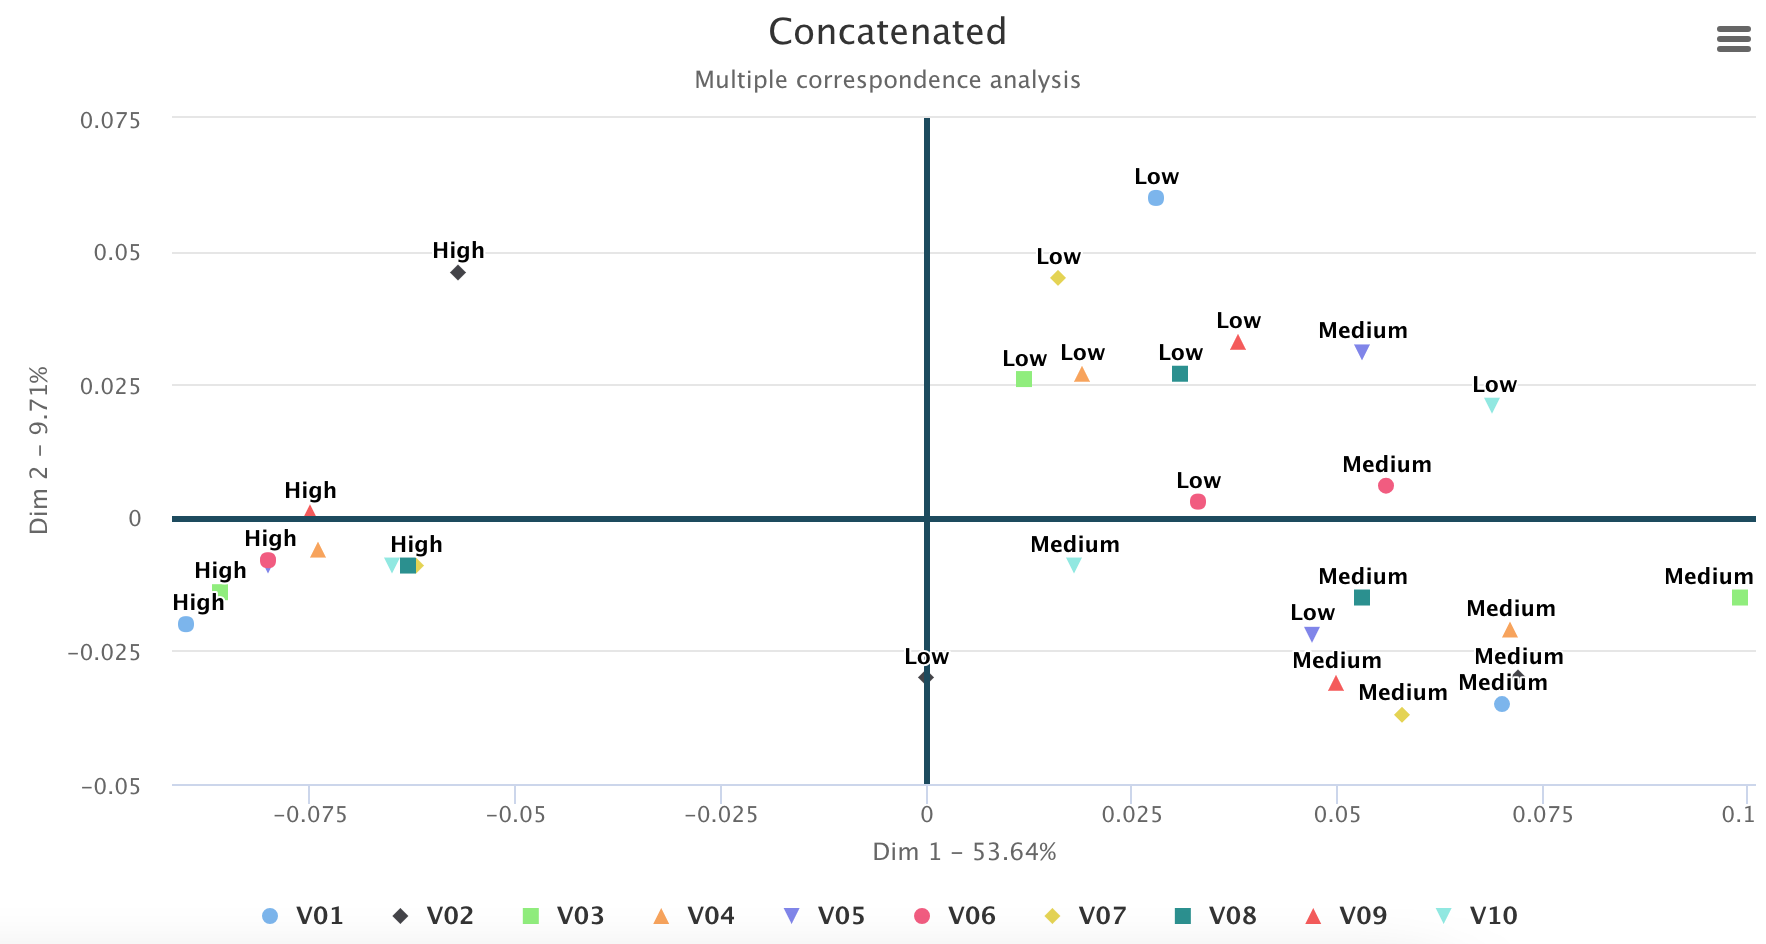
\includegraphics[width=0.9\linewidth,]{concatenated} \end{center}

\caption{Análisis de correspondencias múltiples aplicado a la tabla concatenada.}

\label{fig:concatenatedfig}
\end{figure}

Otro resultado es el Análisis de Correspondencias Múltiples aplicado a
una tabla específica. En este punto, uno de los argumentos que se debe
tener en cuenta es la selección de la tabla con la que se realizará el
análisis.

\begin{figure}[H]


\begin{center}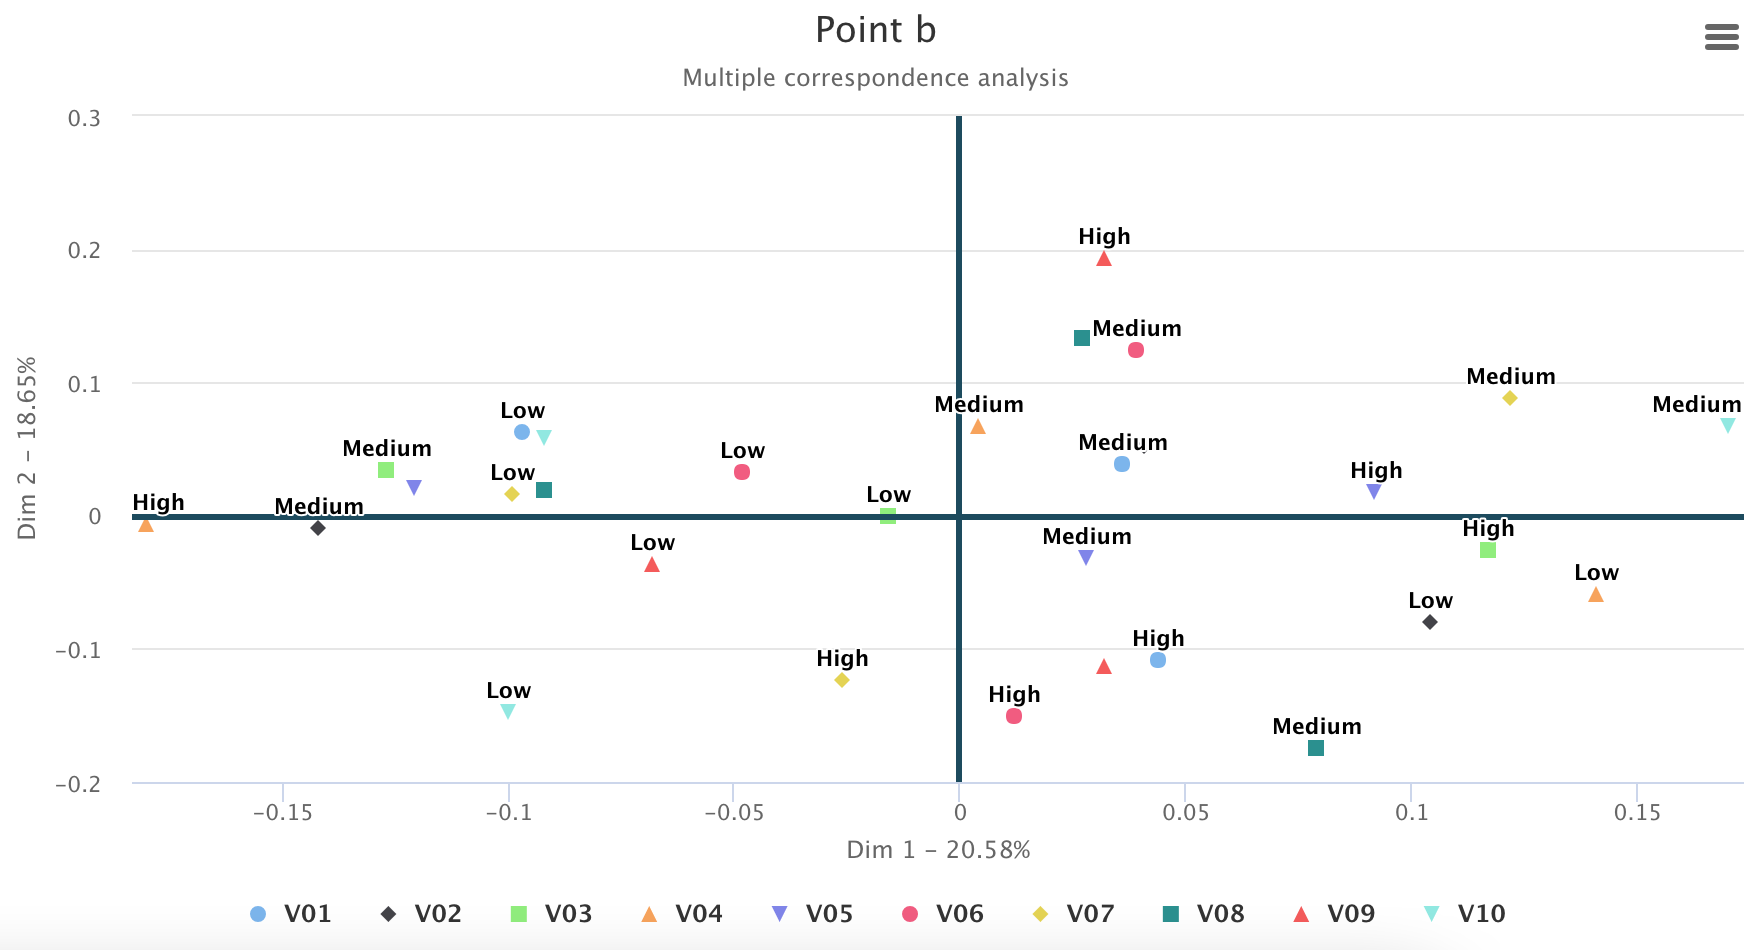
\includegraphics[width=0.9\linewidth,]{pointb} \end{center}

\caption{Análisis de correspondencias múltiples aplicado a la tabla b.}

\label{fig:bfig}
\end{figure}

La figura \ref{fig:bfig} representa el gráfico del MCA de la tabla b.
Este gráfico, en sus dos dimensiones, representa al 39.23\% de la
información. Es notorio que las observaciones en sus niveles alto, medio
y bajo están distribuidas de forma aleatoria en todos los cuadrantes del
gráfico, no se puede precisar un patrón específico de agrupación. Esto
mismo se puede decir de los puntos representados en cualquiera de las
otras tablas porque comparten la misma distribución, exceptuando la
tabla j, que fue diseñada con una distribución diferente. No obstante,
el uso del MCA de las figuras \ref{fig:bfig} y \ref{fig:concatenatedfig}
todavía no permite detectar si el proceso está o no en control. La
identificación de puntos fuera de control se puede realizar mediante la
representación gráfica del estadístico T2 de Hotelling, como se observa
en la figura \ref{fig:tdos}.

\begin{figure}[H]


\begin{center}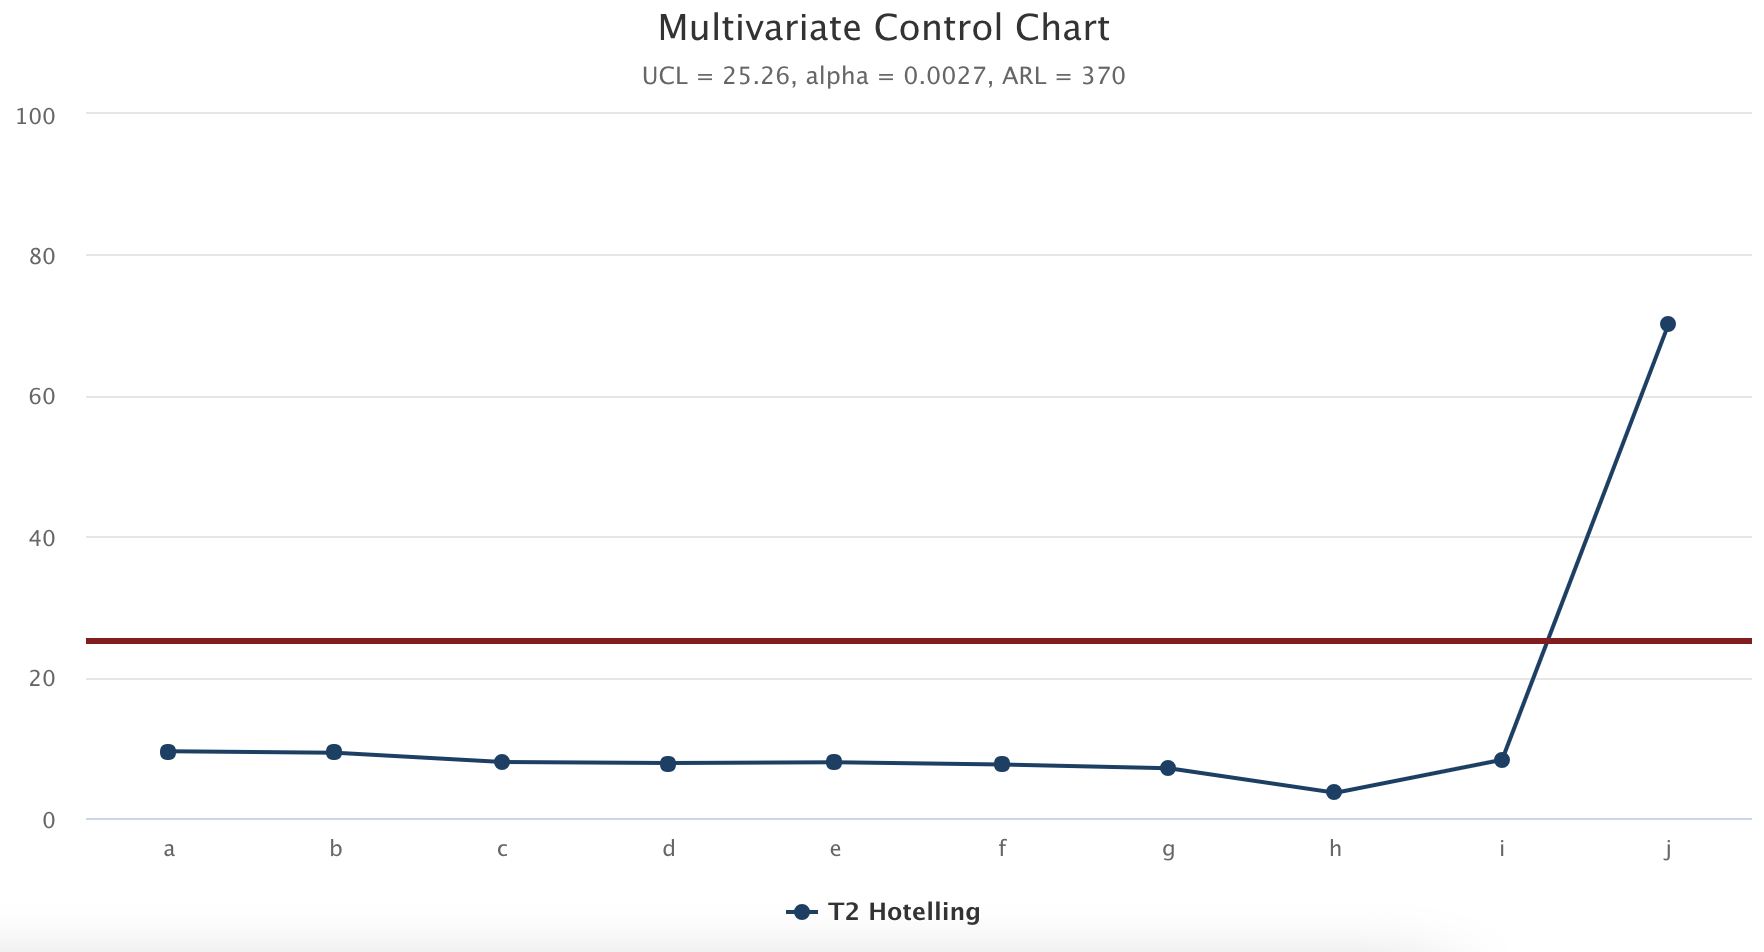
\includegraphics[width=0.9\linewidth,]{t2} \end{center}

\caption{Gráfico de control multivariante T2 Hotelling aplicable a variables cualitativas, $Datak10Contaminated$.}

\label{fig:tdos}
\end{figure}

La figura \ref{fig:tdos} presenta un gráfico de control elaborado con el
estadístico T2 de Hotelling, aplicado a la detección de anomalías en
cualquiera de las \emph{k} tablas analizadas. Cada una de las tablas
está representada por los puntos en el gráfico. Se observa una línea
horizontal que representa al límite de control superior (UCL). El límite
de control inferior (LCL) es igual a cero.

Dado que el análisis de sensibilidad determinó que este gráfico de
control tiene un mejor rendimiento cuando trabaja con un número alto de
dimensiones, se ha recomendado que este número sea \(p-1\), donde
\emph{p} es el número de dimensiones inicial, que es equivalente a la
cantidad de variables de la base de datos, sin contar a la variable
GroupLetter que sólo sirve como factor de clasificación de las tablas.

Se observa que el punto que representa a la tabla \emph{j} se ubica por
encima del límite de control superior, lo que quiere decir que se lo ha
identificado como un valor fuera de control. Por consiguiente, es
necesario analizar con detenimiento qué está pasando con los datos de la
tabla reportada, comparándolos con los de la tabla concatenada, a fin de
identificar las causas de la variación y tomar las acciones pertinentes.
Para hacer un análisis del punto fuera de control se realiza un gráfico
del MCA de la tabla \emph{j} y se lo compara con el gráfico similar de
la tabla concatenada, como se presenta en la figura
\ref{fig:comparation}.

\begin{figure}[H]


\begin{center}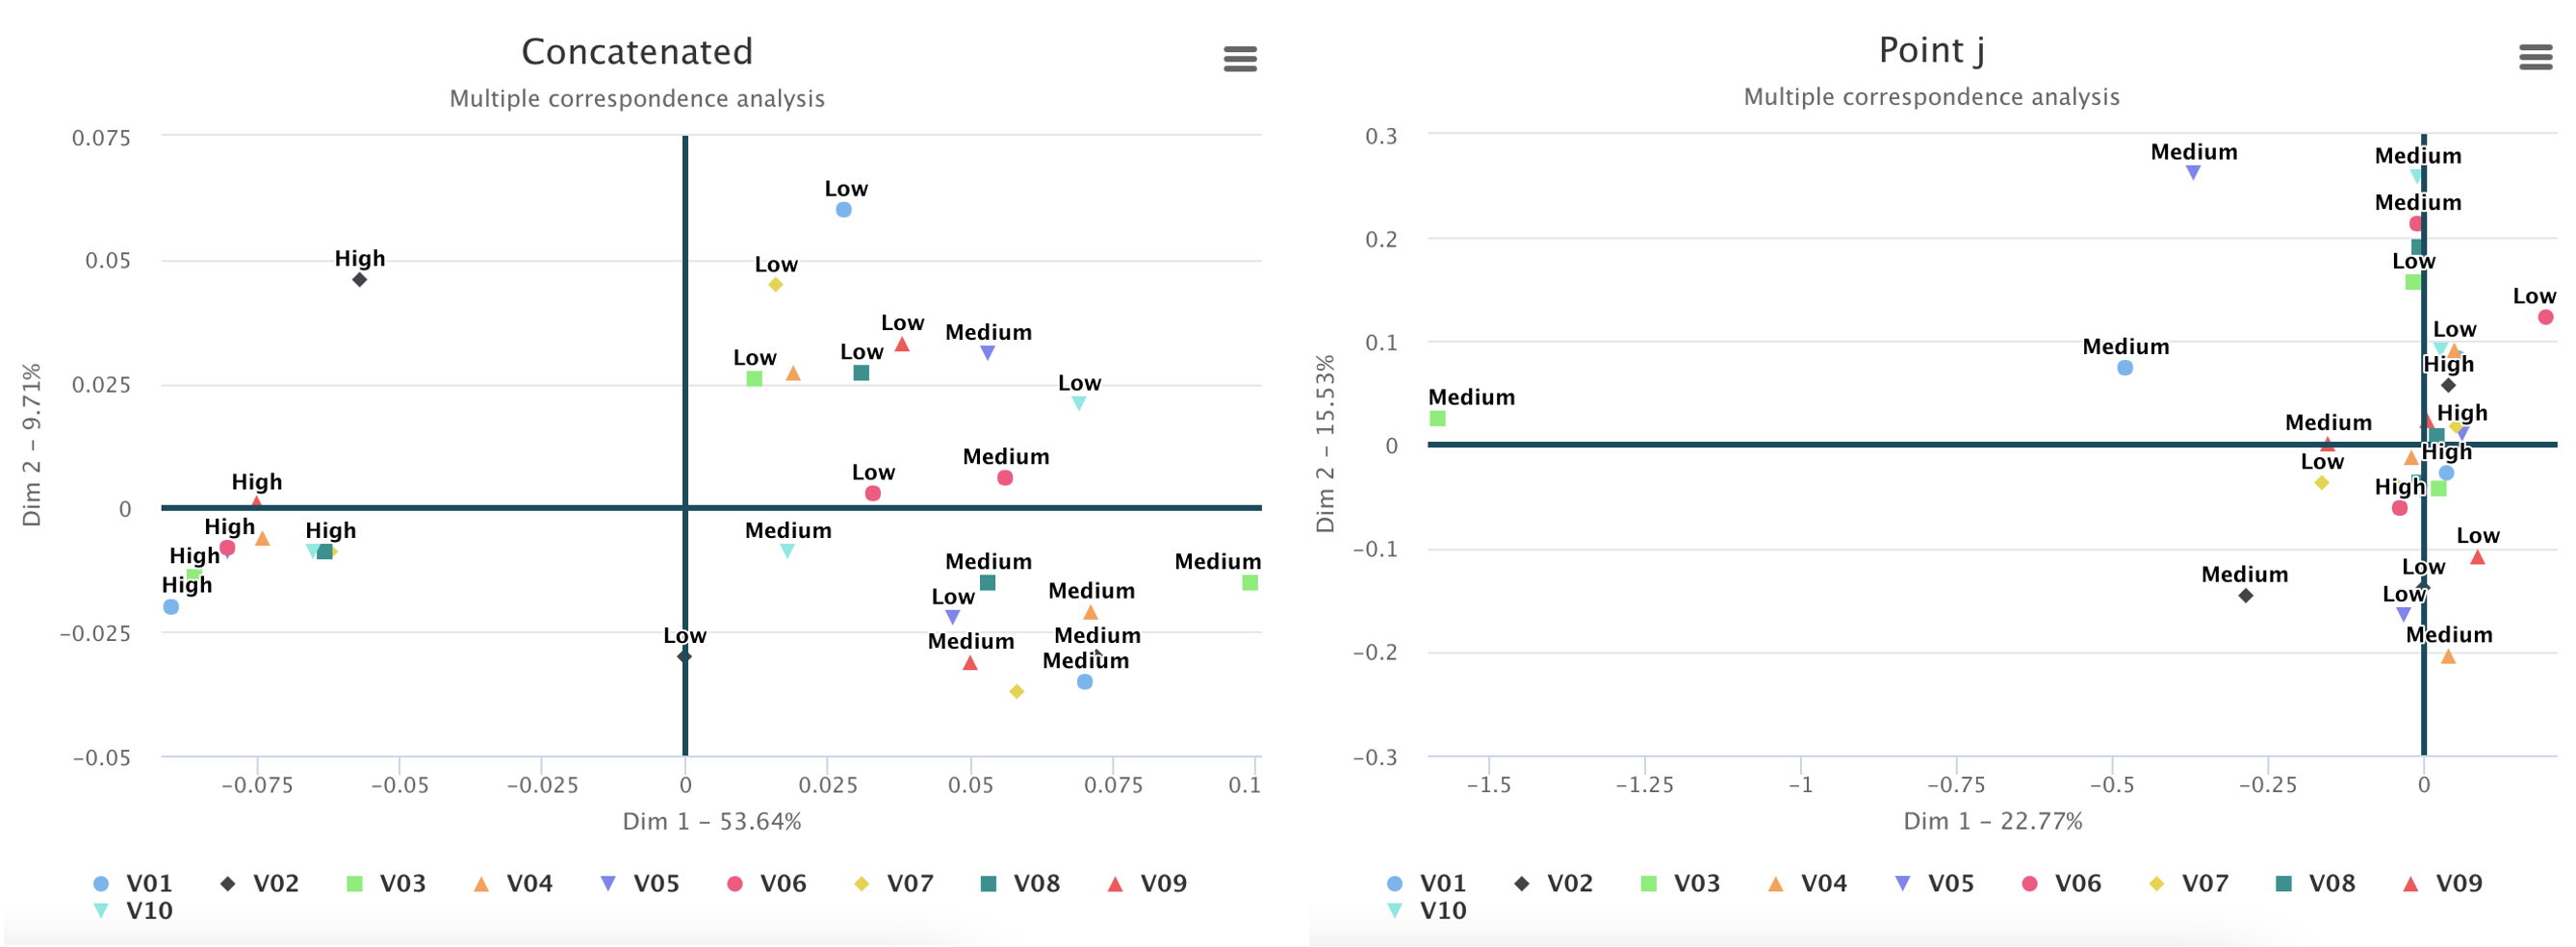
\includegraphics[width=0.9\linewidth,]{comparation} \end{center}

\caption{Gráfico de control multivariante T2 Hotelling aplicable a variables cualitativas, $Datak10Contaminated$.}

\label{fig:comparation}
\end{figure}

La figura \ref{fig:comparation} presenta la distribución de las
observaciones de las tablas concatenada y \emph{j} mediante gráficos del
MCA. El gráfico de la tabla concatenada, que sirve de referente en
control, ya se analizó en la figura 4; el de la tabla \emph{j} muestra
una tendencia de los puntos que con valores medios a ubicarse al lado
izquierdo, bastante alejados de los demás que confluyen hacia el centro
del eje de las X. Especial atención merece la variable 3, que registra
una observación para el nivel medio con el valor más alejado del grupo.

Al comparar los gráficos es evidente que la distribución de los datos en
el gráfico de la tabla \emph{j} es diferente de las distribuciones de
las demás tablas, y en especial, es diferente de la distribución de los
datos en el gráfico de la tabla concatenada, lo que explica por qué el
punto \emph{j} ha sido identificado como fuera de control en el gráfico
T2 de Hotelling. Esta diferencia se explica en la tabla
\ref{tab:chiexamp}, que muestra la distancia Chi cuadrado entre las
observaciones de la tabla concatenada y la tabla \emph{j}.

\begin{table}[H]
\centering
\begin{tabular}{lr}
\toprule
\multicolumn{1}{c}{\cellcolor[HTML]{FFFFFF}{\color[HTML]{000000} \textbf{Variables}}} & \multicolumn{1}{c}{\textbf{ChiSq}} \\ \midrule

\textbf{V1}                                                                             & {\color[HTML]{333333} 0.06968}      \\ 
\textbf{V2}                                                                       & {\color[HTML]{333333} 0.05010}      \\ 
\textbf{V3}                                                                       & {\color[HTML]{333333} 0.07601}      \\ 
\textbf{V4}                                                                       & {\color[HTML]{333333} 0.04982}      \\ 
\textbf{V5}                                                                       & {\color[HTML]{333333} 0.05205}      \\ 
\textbf{V6}                                                                       & {\color[HTML]{333333} 0.05603}      \\ 
\textbf{V7}                                                                       & {\color[HTML]{333333} 0.03713}      \\ 
\textbf{V8}                                                                       & {\color[HTML]{333333} 0.03702}      \\ 
\textbf{V9}                                                                       & {\color[HTML]{333333} 0.04395}      \\ 
\textbf{V10}                                                                            & {\color[HTML]{333333} 0.06179}      \\ \hline
\end{tabular}
\caption{Distancia Chi cuadrado entre las masas de columna de la tabla k y la concatenada, $Datak10Contaminated$.}

\label{tab:chiexamp}
\end{table}

El comportamiento de estas variables en la tabla \emph{j} provoca el
desplazamiento de la tendencia central del proceso que, al final, lo
lleva a un estado fuera de control. Otra manera de visualizar esta
información es a través de un gráfico de barras (figura
\ref{fig:chisqr}).

\begin{figure}[H]


\begin{center}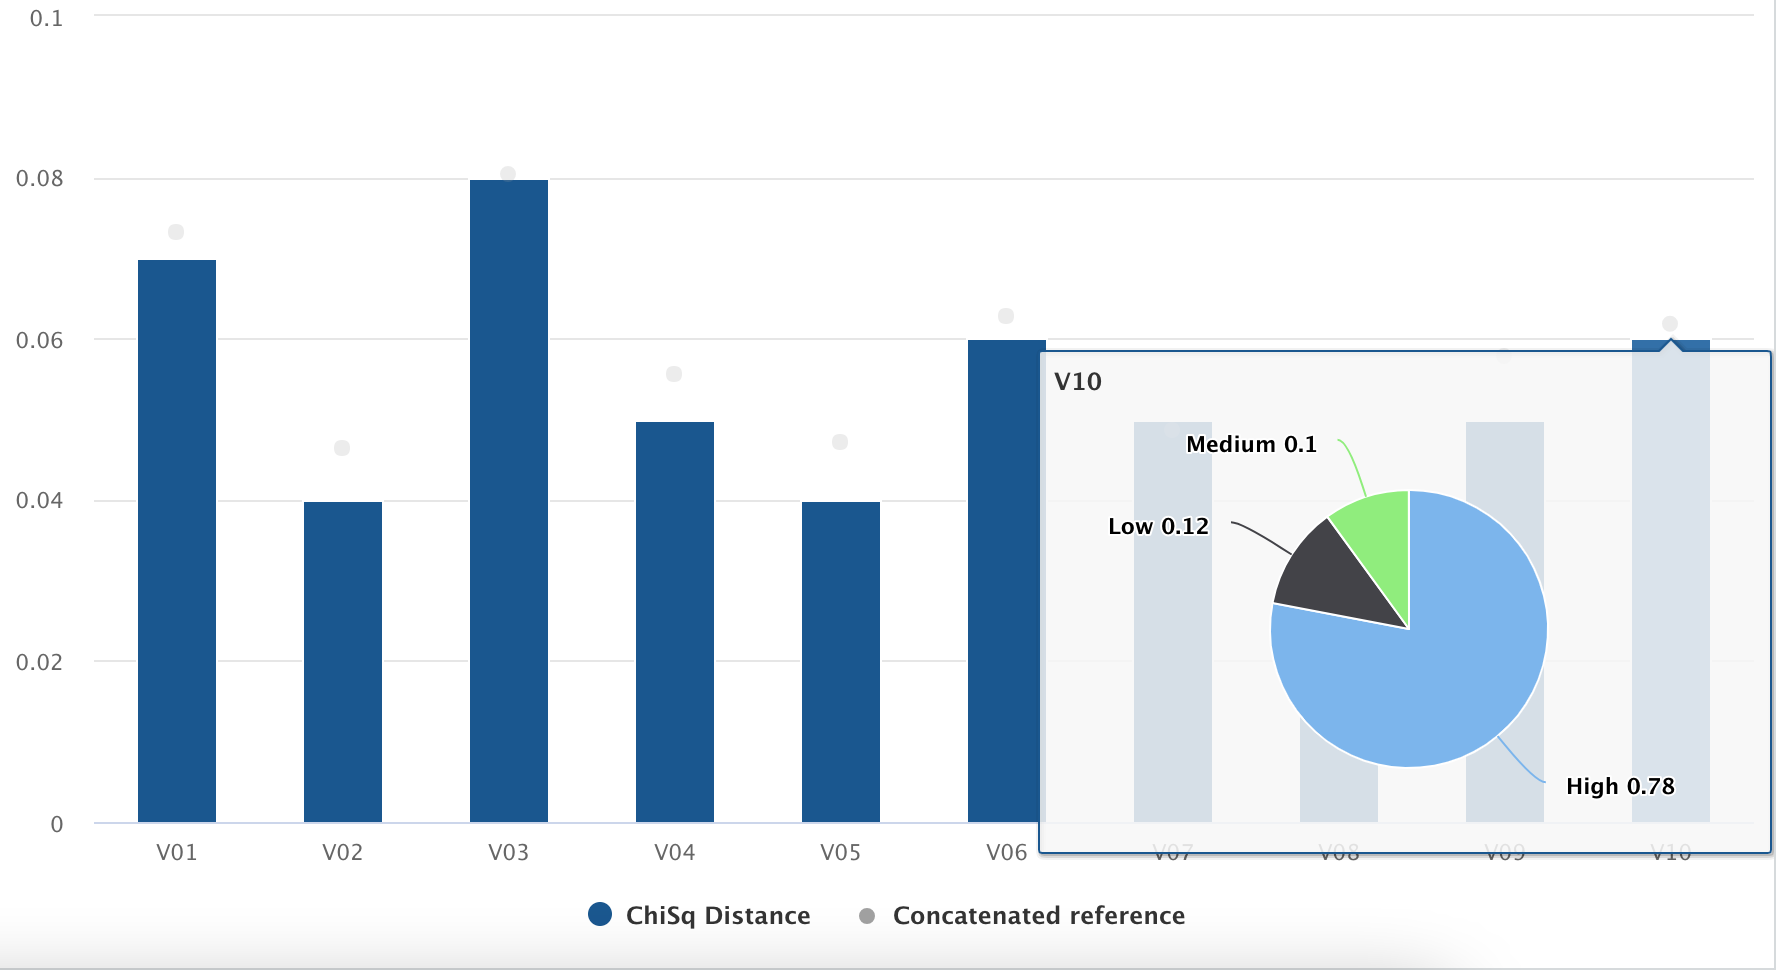
\includegraphics[width=0.9\linewidth,]{Chisqr} \end{center}

\caption{Distancia Chi cuadrado entre las masas de la tabla concatenada y las k tablas, $Datak10Contaminated$.}

\label{fig:chisqr}
\end{figure}

El gráfico de barras de la figura \ref{fig:chisqr}, expresa también la
distancia \(\chi^{2}\) entre las masas de la tabla concatenada y las de
las k tablas de la base de datos \emph{Datak10Contaminated.} Además, la
interactividad de este gráfico facilita la observación de la
distribución de las categorías de las variables de la tabla analizada,
en este caso la j, y su comparación con la distribución de las
categorías de las variables en la tabla concatenada.

\hypertarget{resultados-con-datos-aplicados-al-contexto-de-la-educaciuxf3n-superior}{%
\subsection{Resultados con datos aplicados al contexto de la educación
superior}\label{resultados-con-datos-aplicados-al-contexto-de-la-educaciuxf3n-superior}}

\hypertarget{caracterizaciuxf3n-de-los-datos-aplicados-al-contexto-de-la-educaciuxf3n-superior}{%
\subsubsection{Caracterización de los datos aplicados al contexto de la
educación
superior}\label{caracterizaciuxf3n-de-los-datos-aplicados-al-contexto-de-la-educaciuxf3n-superior}}

En este ejemplo se utiliza una base de datos denominada \emph{bd\_pafd},
tomada de reportes que están disponibles para autoridades de la
Universidad Técnica de Machala (UTMACH) en su Sistema Informático
SIUTMACH. La base de datos \emph{bd\_pafd} contiene 8996 observaciones y
10 variables cualitativas referidas al proceso académico de la carrera
de Pedagogía de la actividad física y deporte, durante 6 periodos
académicos consecutivos, desde 2019-1 hasta 2021-2.

Las variables registradas en la base de datos, con sus respectivas
categorías son las siguientes:

\begin{itemize}
\tightlist
\item
  \textbf{Periodo (periodo)}, esta es la variable que sirve como
  clasificador, hace referencia a los 7 periodos académicos ordinarios
  de estudio (semestres): 2018-2, 2019-1, 2019-2, 2020-1, 2020-2, 2021-1
  y 2021-2.\\
\item
  \textbf{Curso (curso)}, es una variable de caracterización, se trata
  de los diferentes niveles por los que transitan los estudiantes en su
  proceso de formación profesional y son 8. Se los ha identificado con
  números del 1 al 8.\\
\item
  \textbf{Asignatura (asignatura)}, están registradas en la malla
  curricular de la carrera y son 53: Movimientos gimnásticos básicos,
  Cát. Int. Contextos y sistemas pedagógicos, Desarrollo y
  funcionamiento del ser humano, Estructuras y funcionamiento del ser
  humano, PEA Comunicación humana, Investigación y acción cooperativa,
  PEA Natación, Movimientos gimnásticos reglamentados, Cát. Int.
  Contextos y sistemas didácticos, Desarrollo psicológico, Expresión
  Corporal, Investigación acción participativa, Atletismo, PEA hab.
  motoras básicas, Teoría y práctica de los juegos I, Cát. Int. Modelos
  Educación Corporal, Psicopedagogía de la Act. física y deporte,
  Introducción a la Comunicación Científica, Inv. Educ. Fundamentos
  básicos, Atletismo, PEA hab. motoras condicionantes, Fundamentos de la
  Recreación, Cát. Int. PEA Educación Inicial, Ofimática Aplicada, Inv.
  Educ. Diagnóstico, Teoría y práctica de los Juegos II, PEA Fútbol, PEA
  Tae Kwon Do, Cát. Int. PEA Educación Básica, Danza y manifestaciones
  artísticas interculturales, Inv. Educ. Diseño y planificación,
  Ofimática Aplicada II, Teoría y metod. entrenamiento deportivo,
  Comunicación académica, Investigación científica, Comunicación
  académica II, Danza y expresión corporal, Cát. Int. PEA Bachillerato,
  Estadística aplicada, Gestión escolar y DP docente, Lectura y
  escritura de textos académicos, PEA Baloncesto, Tecn. Información y
  Comunicación, Cát. Int. Contextos y sistemas pedagógicos, Cát. Int.
  Contextos y sistemas didácticos, Cát. Int. PEA Inclusivo, Fútbol sala,
  PEA Voleibol, Seminario de titulación I, Teoría curricular y
  evaluación educ., Cát. Int. Gestión de proyectos, Masificación
  deportiva escolar, Musculación, Normativa del deporte y políticas
  educativas, Seminario de titulación II.\\
\item
  \textbf{Código docente (cod\_docente)}, es el código que reemplaza a
  los nombres de cada uno de los 36 docentes de las diferentes
  asignaturas que han sido impartidas a lo largo de los 6 periodos
  académicos estudiados. Los códigos son: DH16, DM02, DH19, DH06, DM18,
  DH17, DM13, DH02, DH08, DM07, DH03, DH21, DH04, DH13, DH01, DM01,
  DM12, DH10, DH05, DM16, DH14, DH15, DH20, DM15, DH07, DM11, DH18,
  DM14, DH12, DH23, M06, DM09, DM17, DM05, DM10, DM03.\\
\item
  \textbf{Capacitación docente (niv\_capacitacion)}, es una variable de
  control que se expresa en cuatro niveles: la categoría \emph{Alto}
  agrupa a profesores que durante el periodo estudiado, además de haber
  recibido capacitación en temas de interés académico y dados por la
  universidad, recibieron por su iniciativa (fuera de la universidad)
  cursos en temas relacionados con su profesión; en el nivel \emph{Medio
  alto} están los profesores que, durante el periodo de estudio, sólo
  recibieron cursos de capacitación dados por la universidad; en el
  nivel \emph{Medio bajo}, los que durante el periodo de estudio sólo se
  capacitaron en temas de su profesión en eventos impartidos por
  organizaciones distintas a la UTMACH. Finalmente, el nivel \emph{Bajo}
  corresponde a profesores que durante el periodo de estudio no
  recibieron capacitación, aunque sí la tenían en periodos anteriores.\\
\item
  \textbf{Seguimiento al sílabo (seg\_silabo)}, es otra variable de
  control, valora la medida en que se ha cumplido el proceso de
  seguimiento del sílabo de las asignaturas establecidas en la malla
  curricular, con la participación de estudiantes y profesores. Los
  niveles establecidos son cinco: \emph{Completo, Mayoritario, Moderado,
  Escaso} y \emph{Sin seguimiento.}\\
\item
  \textbf{Avance académico (avance\_acad)}, esta variable de control es
  reportada en el SIUTMACH por los docentes y contrastada por los
  estudiantes en el proceso de seguimiento al sílabo. Indica en qué
  medida se ha cumplido los contenidos planificados para las
  asignaturas. Los niveles establecidos son cuatro: \emph{Completo,
  Mayoritario, Moderado} y \emph{Escaso.}\\
\item
  \textbf{Asistencia a clases (asistencia)}, expresa, en cuatro niveles,
  el nivel asistencia a clases por parte de los estudiantes, las
  categorías de esta variable de control son: \emph{Asistencia total,
  Casi no falta, A veces falta, Muchas veces falta} y \emph{Falta
  demasiado.}\\
\item
  \textbf{Calificación (calif\_q)}, se considera como una variable de
  respuesta que representa el rendimiento académico alcanzado por los
  estudiantes, expresado en una escala cualitativa, sus categorías son:
  Excelente, que corresponde a valores numéricos de 9.00 a 10; \emph{Muy
  bueno}, con valores de 8.00 a 8.99; \emph{Bueno}, de 7.00 a 7.99;
  \emph{Regular}, de 6.00 a 6.99 y \emph{Deficiente}, con valores
  menores que 6.00.\\
\item
  \textbf{Estado (estatus)}, es otra variable de respuesta, indica en
  cuatro niveles, en qué estado queda el estudiante al término del
  periodo académico. Las categorías de esta variable son: \emph{Aprueba
  directo}, \emph{Aprobado con recuperación}, \emph{Reprobado por
  faltas} y \emph{Reprobado por notas}.
\end{itemize}

\hypertarget{aplicaciuxf3n-del-paquete-t2qv-con-datos-del-contexto-de-la-educaciuxf3n-superior}{%
\subsubsection{Aplicación del paquete T2Qv con datos del contexto de la
educación
superior}\label{aplicaciuxf3n-del-paquete-t2qv-con-datos-del-contexto-de-la-educaciuxf3n-superior}}

El gráfico del Análisis de Correspondencias Múltiples que se realiza a
la tabla concatenada (Figura \ref{fig:concatedu}) es el escenario que se
utilizará como referente para el análisis de las tablas que, en el
gráfico T2 de Hotelling, se registren como puntos fuera de control o con
otras tablas que merezcan el interés del investigador.

El gráfico del MCA de la tabla concatenada que presenta el aplicativo
T2Qv ofrece dos versiones, una fija y otra interactiva, ésta permite
ingresar una a una las variables, lo que facilita el análisis de la
asociación entre categorías. Aquí se presenta el gráfico en su versión
interactiva. Los puntos representan a las observaciones de cada una de
las 10 variables en sus distintos niveles. La variable periodo sirve
como elemento clasificador, por eso sus observaciones no aparecen aquí.

\begin{figure}[H]


\begin{center}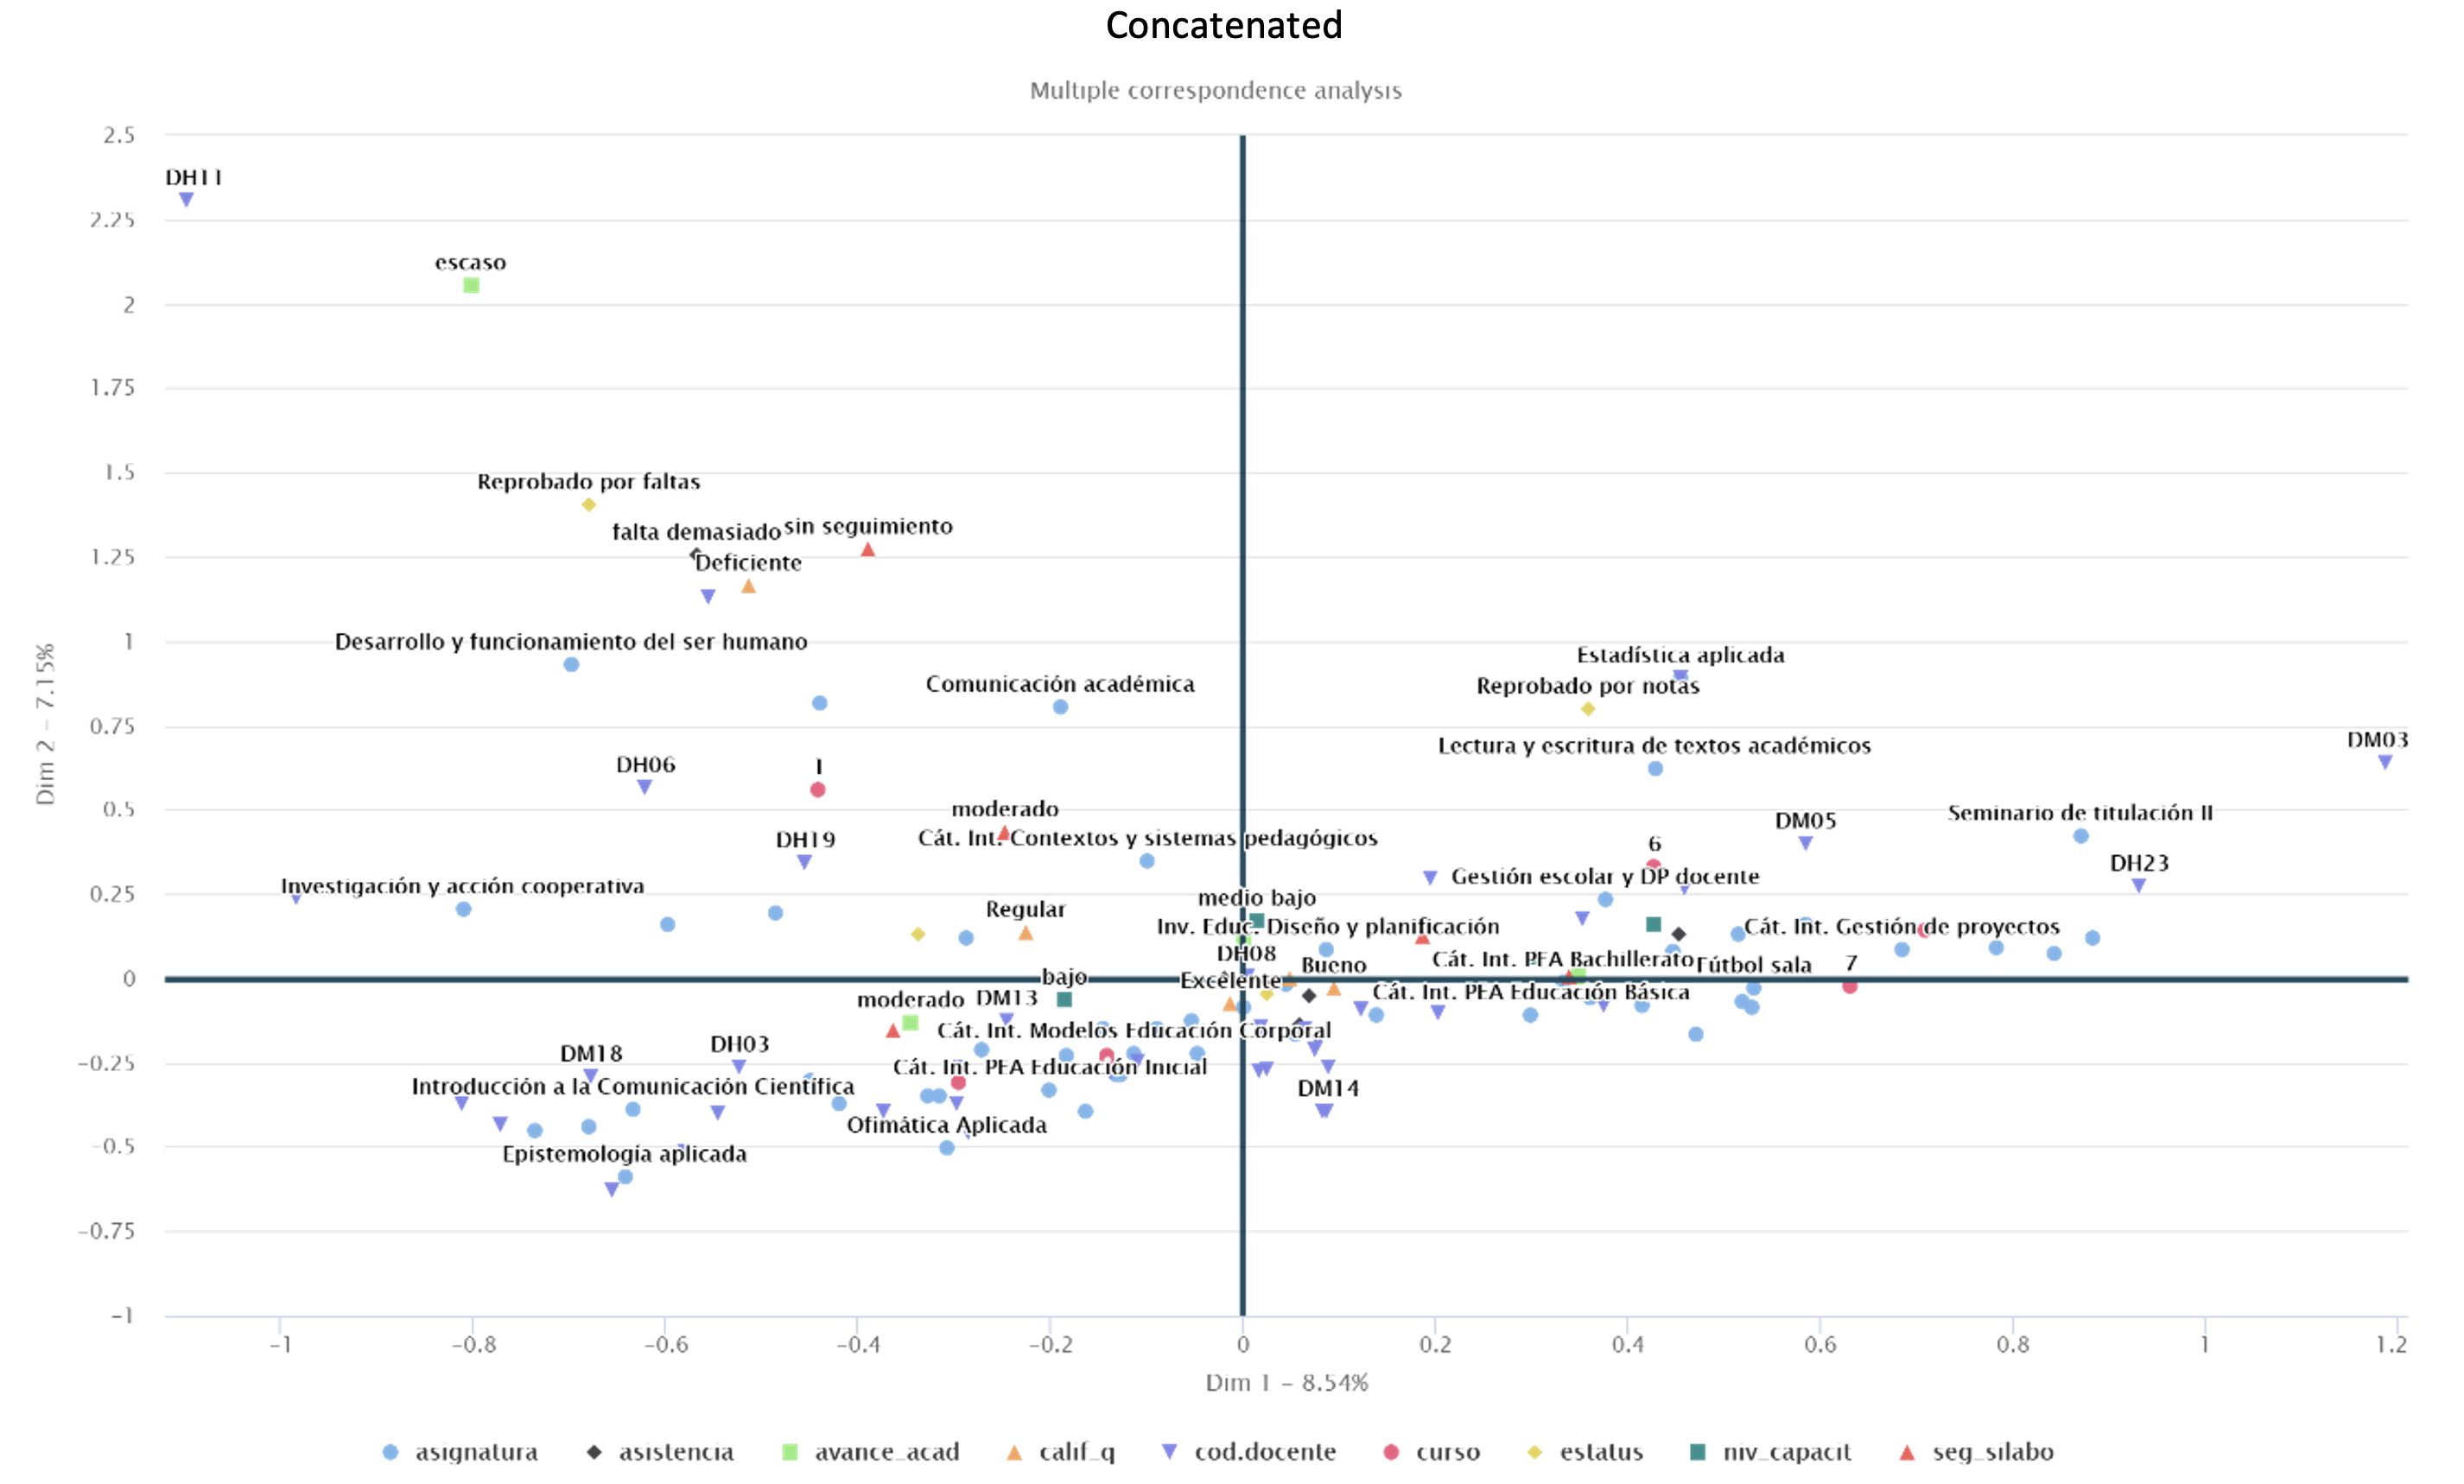
\includegraphics[width=0.9\linewidth,]{concat_edu} \end{center}

\caption{Gráfico de MCA de la tabla concatenada $bd$ $pafd$.}
\label{fig:concatedu}
\end{figure}

El MCA reporta una inercia total del 15.69\%, valor que a primera vista
no entusiasma demasiado. Se trata de un análisis bastante complejo y de
alta variabilidad, por el alto número de variables y categorías con
información de estudiantes, de profesores, de asignaturas, de prácticas
académicas, de 7 periodos académicos en una carrera universitaria. El
bajo porcentaje de variabilidad explicada podría generar insuficiencias
en la interpretación de la ubicación de los puntos, mas, no se puede
esperar que toda la variabilidad sea capturada de forma mayoritaria sólo
por dos dimensiones. Por otra parte, la nube de puntos sí refleja la
asociación entre las categorías de las variables analizadas.

La figura \ref{fig:concatedu} muestra la nube de puntos de las variables
que corresponden al gráfico de MCA de la tabla concatenada Se observa
que en el centro del gráfico confluyen las categorías \emph{Excelente,
Muy bueno} y \emph{Bueno} de la variable calif\_q, las categorías
\emph{Asistencia total} y \emph{Casi no falta }de la variable
Asistencia, además, la categoría \emph{Aprueba directo} de la variable
estatus. Estos resultados aparecen con mayor frecuencia, lo que indica
que la mayoría de los estudiantes ha asistido normalmente a clases y ha
obtenido un rendimiento académico igual o superior a 7/10, que
constituye el requisito para aprobar las asignaturas de forma directa,
sin necesidad de exámenes de supletorio o recuperación. Entre estas
asignaturas están Metodología de la enseñanza aprendizaje del Fútbol,
Contextos y sistemas didácticos, Danza y expresión corporal y Atletismo,
Habilidades motoras básicas.

Por su parte, el estatus de \emph{Aprobado con recuperación} se asocia
con la calificación de \emph{Regular.} Estas categorías están un poco
alejadas del centro, lo que significa que son menos los casos de
estudiantes que por su bajo rendimiento académico han tenido que acudir
a exámenes de recuperación (supletorio) para aprobar las asignaturas que
los casos de estudiantes que aprueban directo. Entre las asignaturas de
este grupo están Teoría y métodos de entrenamiento deportivo y Enseñanza
y aprendizaje de la comunicación humana.

La categoría \emph{Reprobado por faltas} se asocia con la de \emph{Falta
demasiado} y con calificaciones de \emph{Deficiente.} Esto se explica
porque ha habido casos de estudiantes que por faltar demasiado a clases
no han podido consolidar su aprendizaje, lo que ha provocado que
obtengan calificaciones menores que 6/10, equivalentes a un nivel de
\emph{deficiente}, además de que sobrepasaron el límite permitido de
inasistencia a clases, que es de 10\%, lo que ha dado como resultado que
reprueben asignaturas por faltas. Afortunadamente la ubicación de estas
observaciones está bastante alejada del centro del gráfico, lo que
indica que hay pocos de estos casos, por ejemplo, en la asignatura de
Desarrollo y funcionamiento del ser humano. En el ACM, las categorías
poco comunes se ubican lejos del origen, la distancia se incrementa con
la rareza.

La categoría \emph{Reprobado por notas} se aleja del centro del gráfico
y, aunque de una manera no tan cercana, se relaciona con la de
\emph{Muchas veces falta}. Es el caso de estudiantes que mostraron un
escaso desarrollo de aprendizajes, quizás por inasistencia frecuente a
clases, falta de prerrequisitos, quizás por otros motivos y, en
consecuencia, tuvieron bajas calificaciones que no permitieron aprobar
las asignaturas ni siquiera con exámenes de recuperación. Entre estas
asignaturas están Estadística aplicada y Lectura y escritura de textos
académicos.

Al introducir al análisis la variable Avance académico se observa que
los mejores resultados se dan cuando el avance llega a
\emph{Mayoritario}, es decir, cuando se ha cumplido la mayor parte de
los contenidos y objetivos planificados, aunque no su totalidad, como es
el caso de Comunicación académica II. El avance \emph{Completo} está más
cerca de asignaturas cuyos estudiantes reprueban por notas (Gestión
escolar y desarrollo profesional docente), mientras que, el avance
\emph{Moderado} se asocia con asignaturas que se aprueban mediante
exámenes de recuperación (Enseñanza aprendizaje de la Actividad Física y
Deporte en la Educación Inicial).

Parecería que cuando los profesores intentan cumplir todos los temas
planificados, aunque no hayan podido desarrollar adecuadamente el
proceso de enseñanza aprendizaje, se producen resultados más bajos que
cuando se avanza la mayor parte del sílabo pero llegando a una
consolidación del aprendizaje, aunque algunos temas puedan quedar sin
estudiarse.

La variable Seguimiento al sílabo, cuya responsabilidad recae
mayoritariamente en los estudiantes, demuestra una lógica asociación con
la variable Avance académico, que reportan los docentes. Así, la
categoría de avance académico \emph{Completo} se asocia con mucha fuerza
al seguimiento al sílabo \emph{Completo} (Enseñanza aprendizaje de la
actividad física y deporte en el bachillerato) y un poco menos al
seguimiento al sílabo \emph{Mayoritario}; el avance académico
\emph{Moderado} se relaciona mucho con el seguimiento al sílabo
\emph{Escaso} (Expresión corporal) y un poco menos con la categoría de
\emph{Moderado.}

En cuanto a la variable Capacitación docente, sus niveles más altos
están asociados con asignaturas que tuvieron avance académico y
seguimiento al sílabo \emph{Completo.} En este caso se expresa un alto
grado de formalidad y cumplimiento, porque los profesores recibieron
capacitación planificada y ejecutada por la universidad y el sílabo se
ejecutó en su totalidad, por ello su seguimiento fue reportado como
completo por estudiantes y profesores. Como ejemplo se tiene a los
profesores identificados con los códigos y asignaturas siguientes: DM10
(Tecn. Información y Comunicación, 6to semestre), DH01 (Cát.
Integradora, enseñanza aprendizaje de la Actividad Física y Deporte en
la Educación General Básica, 5to semestre). Sin embargo, los resultados
académicos alcanzados por los estudiantes en este grupo no son los más
altos.

Los resultados académicos más altos, donde los estudiantes aprueban las
asignaturas de forma directa, se asocian a un nivel de capacitación
docente \emph{Medio bajo}, es decir, profesores que se capacitan más en
temas específicos de su carrera (deportes, entrenamiento) que en temas
académicos impartidos regularmente por la universidad. Se debe observar
que en este grupo, los profesores no cumplieron totalmente el sílabo,
sino sólo a un nivel \emph{Mayoritario.} En este grupo están los
profesores DH14 (Investigación educativa: Diseño y planificación de la
investigación, 5to semestre) y DH08 (Metodología de la enseñanza
aprendizaje del Fútbol, 5to semestre).

\begin{figure}[H]


\begin{center}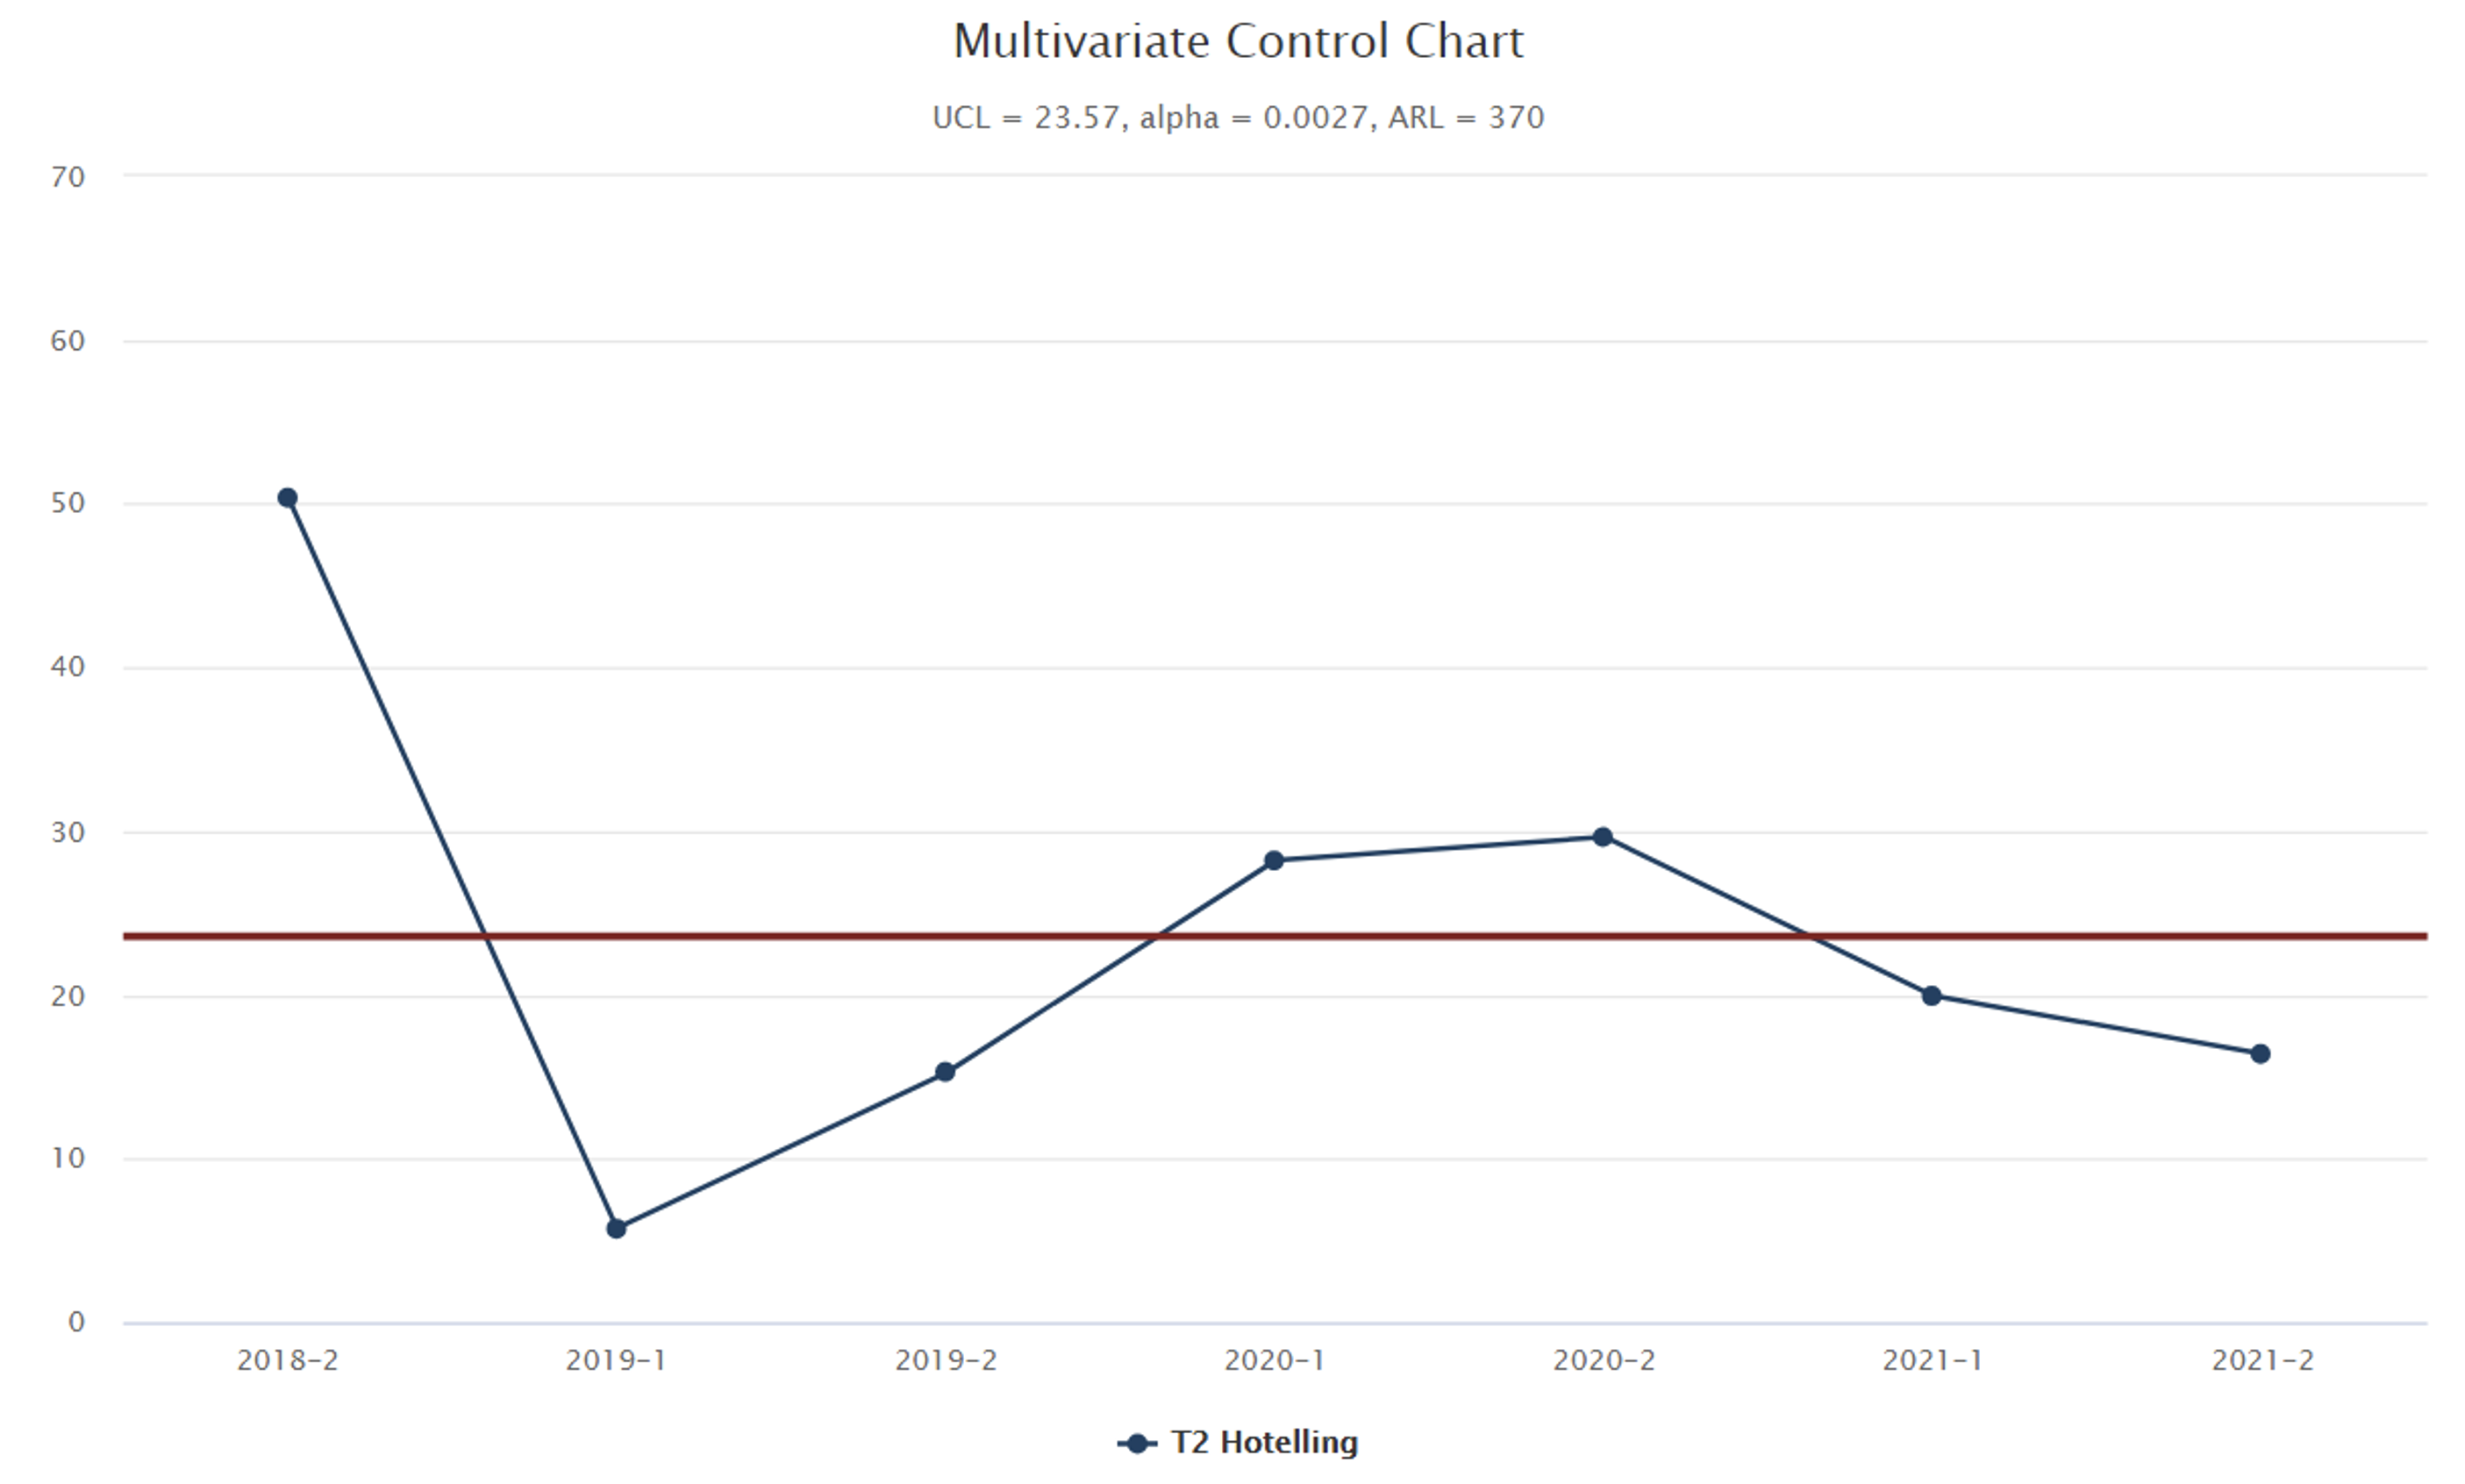
\includegraphics[width=0.9\linewidth,]{tdos_edu} \end{center}

\caption{Gráfico de control multivariante T2 Hotelling aplicable a variables cualitativas, $bd$ $pafd$.}
\label{fig:tdosedu}
\end{figure}

La figura \ref{fig:tdosedu} muestra el gráfico de control T2 de
Hotelling para la representación de las k = 7 tablas analizadas, éstas
se representan por los puntos del gráfico y corresponden a los siete
periodos académicos considerados en este estudio. Tres puntos han sido
detectados como fuera de control: 2018-2, 2020-1 y 2020-2, en
consecuencia, será necesario un análisis de sus datos comparados con los
de la tabla concatenada para identificar las causas de la variación y
facilitar la toma de decisiones que permitan corregir las desviaciones
encontradas. Para ello se hará gráficos del MCA de las tablas señaladas,
lo que implica seleccionar en el aplicativo T2Qv la tabla que se desea
comparar con la concatenada.

\begin{figure}[H]


\begin{center}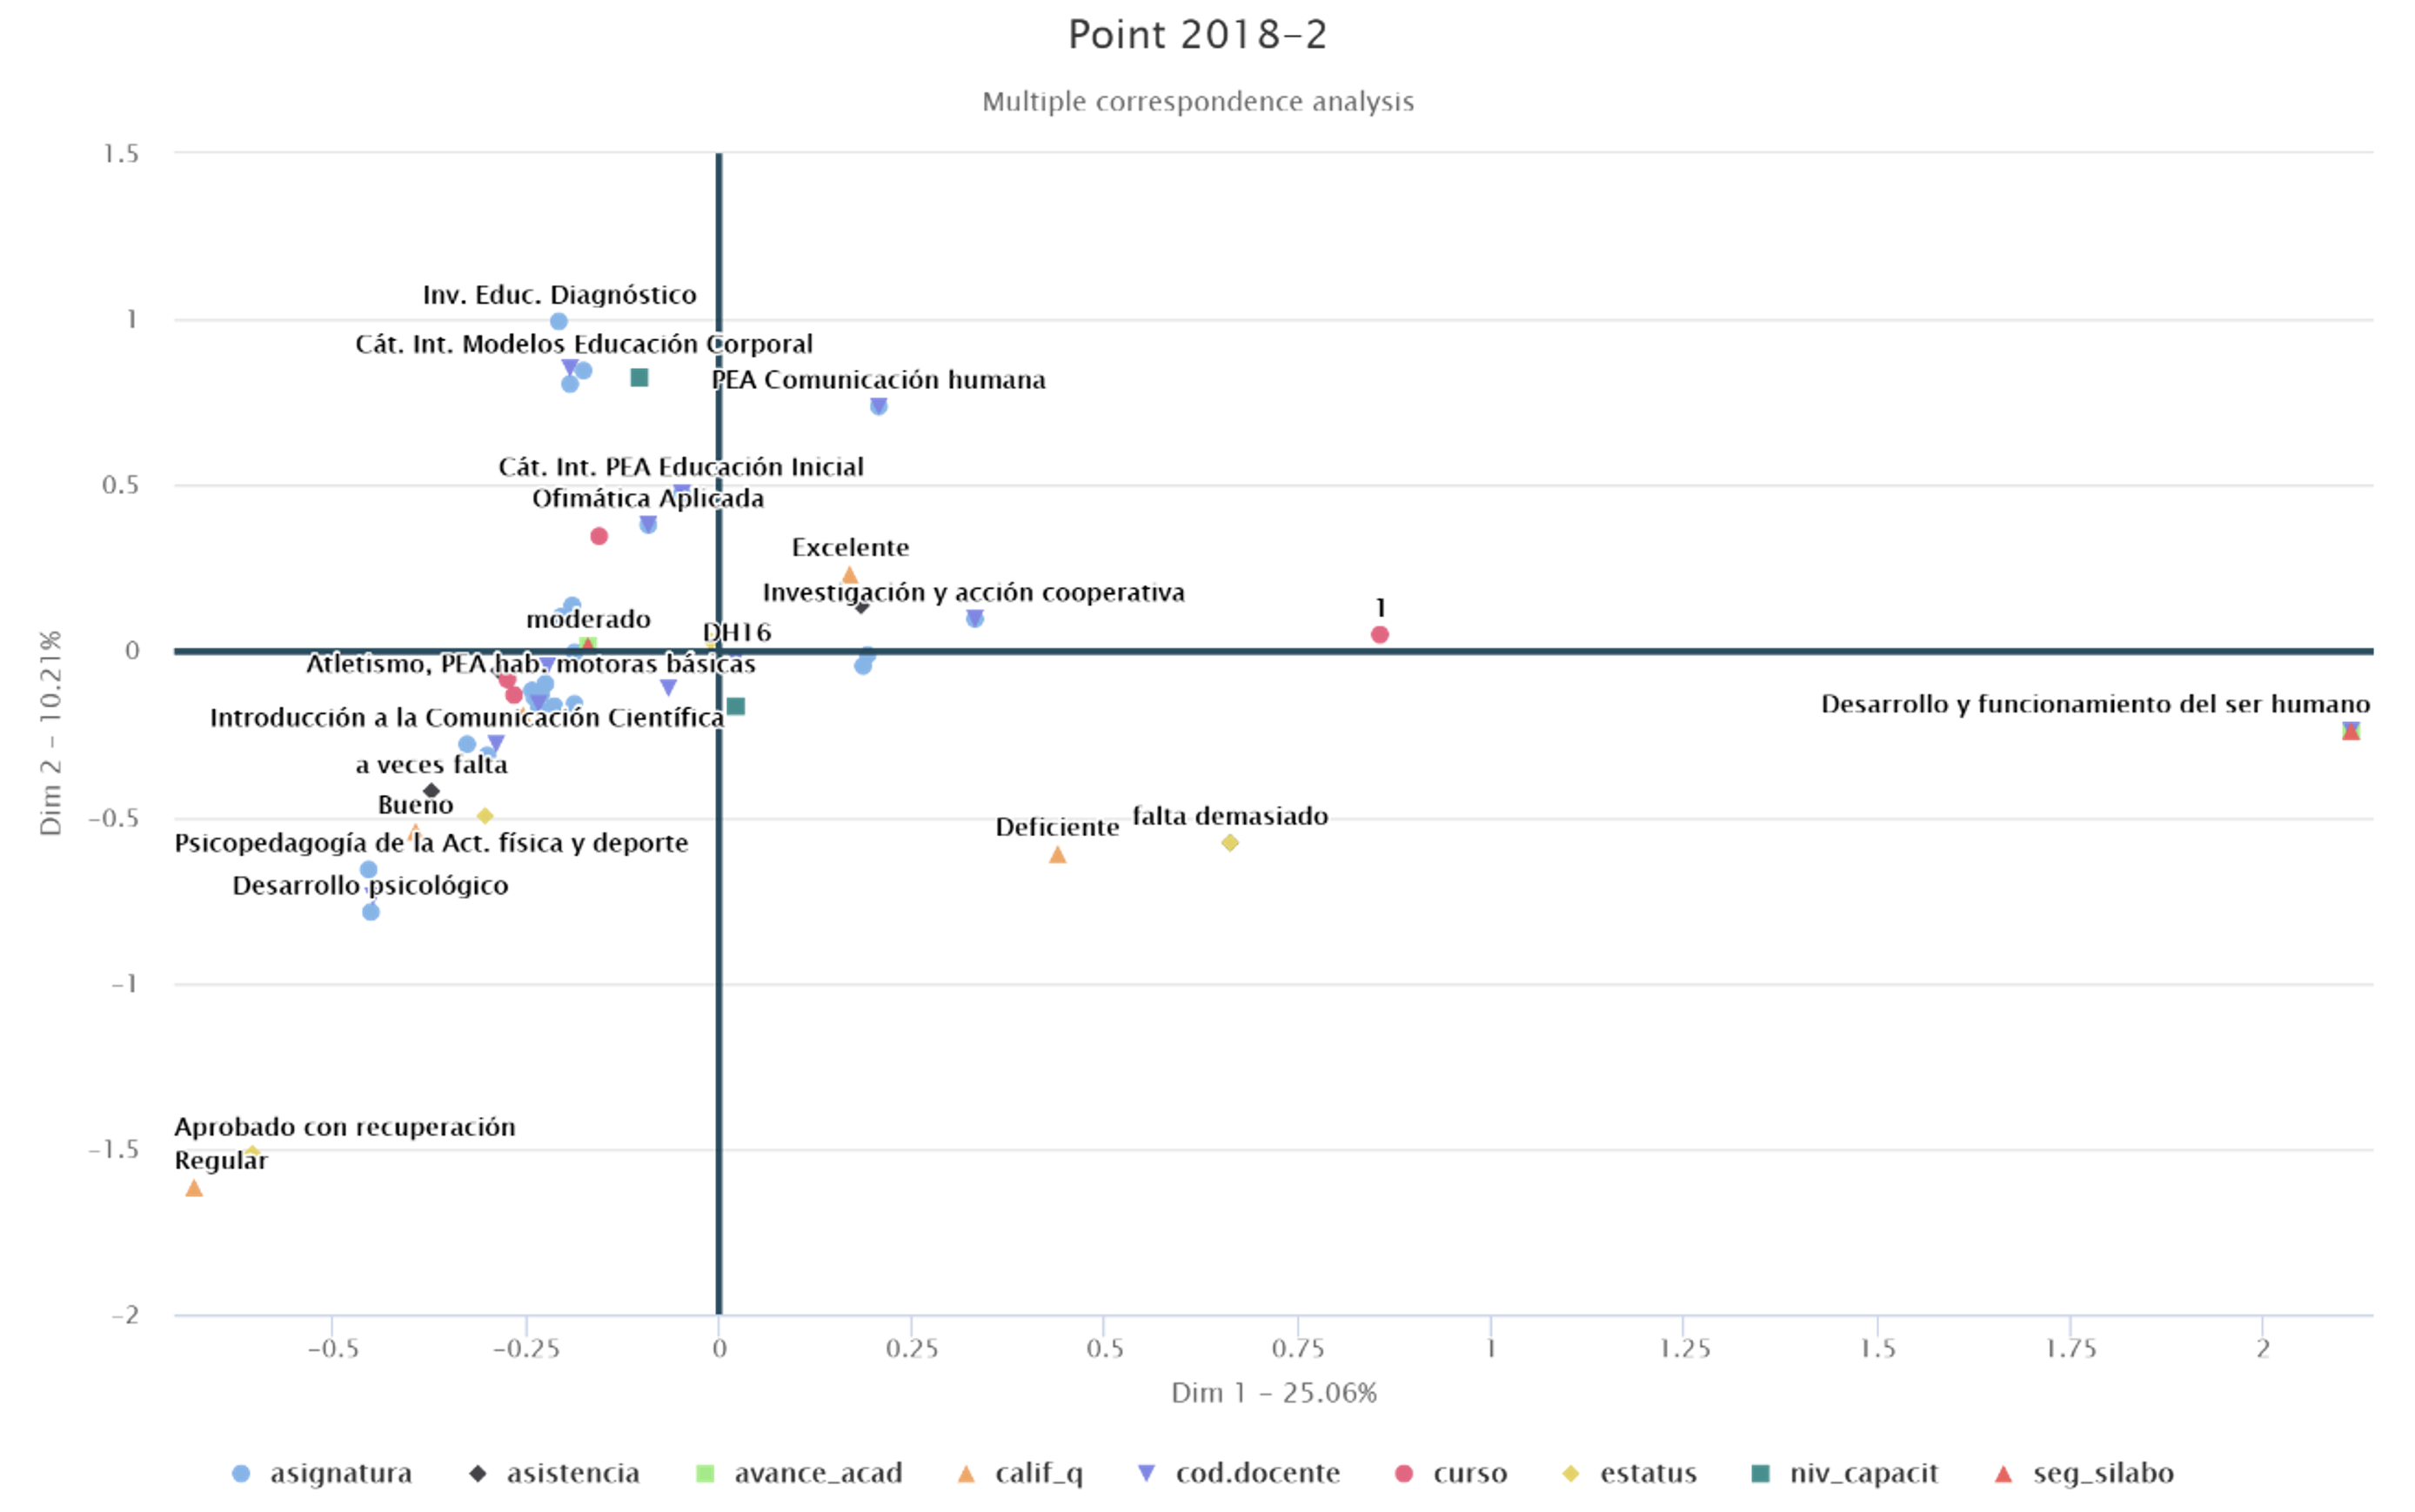
\includegraphics[width=0.9\linewidth,]{point2018_edu} \end{center}

\caption{Gráfico de MCA de la tabla 2018-2, $bd$ $pafd$.}
\label{fig:point2018edu}
\end{figure}

La figura \ref{fig:point2018edu} contiene el gráfico del MCA de la tabla
2018-2. La varianza explicada en sus dos dimensiones es 35.27\%. El
gráfico proporciona una idea clara de la asociación entre categorías de
las variables, además, si se revisa el gráfico de barras generado por el
aplicativo informático T2Qv (figura 13), se puede reconocer la
distribución interna de la variable, lo que ayuda a la identificación de
las diferencias entre la tabla concatenada y la analizada, en este caso
2018-2.

Para interpretar estas diferencias, hay que decir que Pedagogía de la
Actividad física y deporte es una carrera nueva, que se inauguró en el
periodo 2017-1 con el primer semestre y fue avanzando periodo a periodo,
de manera que en 2018-2 sólo tenía 4 semestres desarrollados de los 8
establecidos en su diseño curricular. Por esta razón, la tabla
concatenada registra 52 asignaturas y 40 profesores, mientras que la
tabla 2018-2, sólo 25 y 12, respectivamente. Esto ha generado cambios en
la distribución de las categorías de las diferentes variables, como
calif\_q, seg\_silabo, asistencia, niv\_capacit. Los cambios se aprecian
mejor si se analizan de forma simultánea los gráficos de la tabla
concatenada y la 2018-2. La figura \ref{fig:compedu} presenta estos
gráficos que, para facilitar la comparación, se generan de forma
conjunta en el aplicativo informático T2Qv.

\begin{figure}[H]


\begin{center}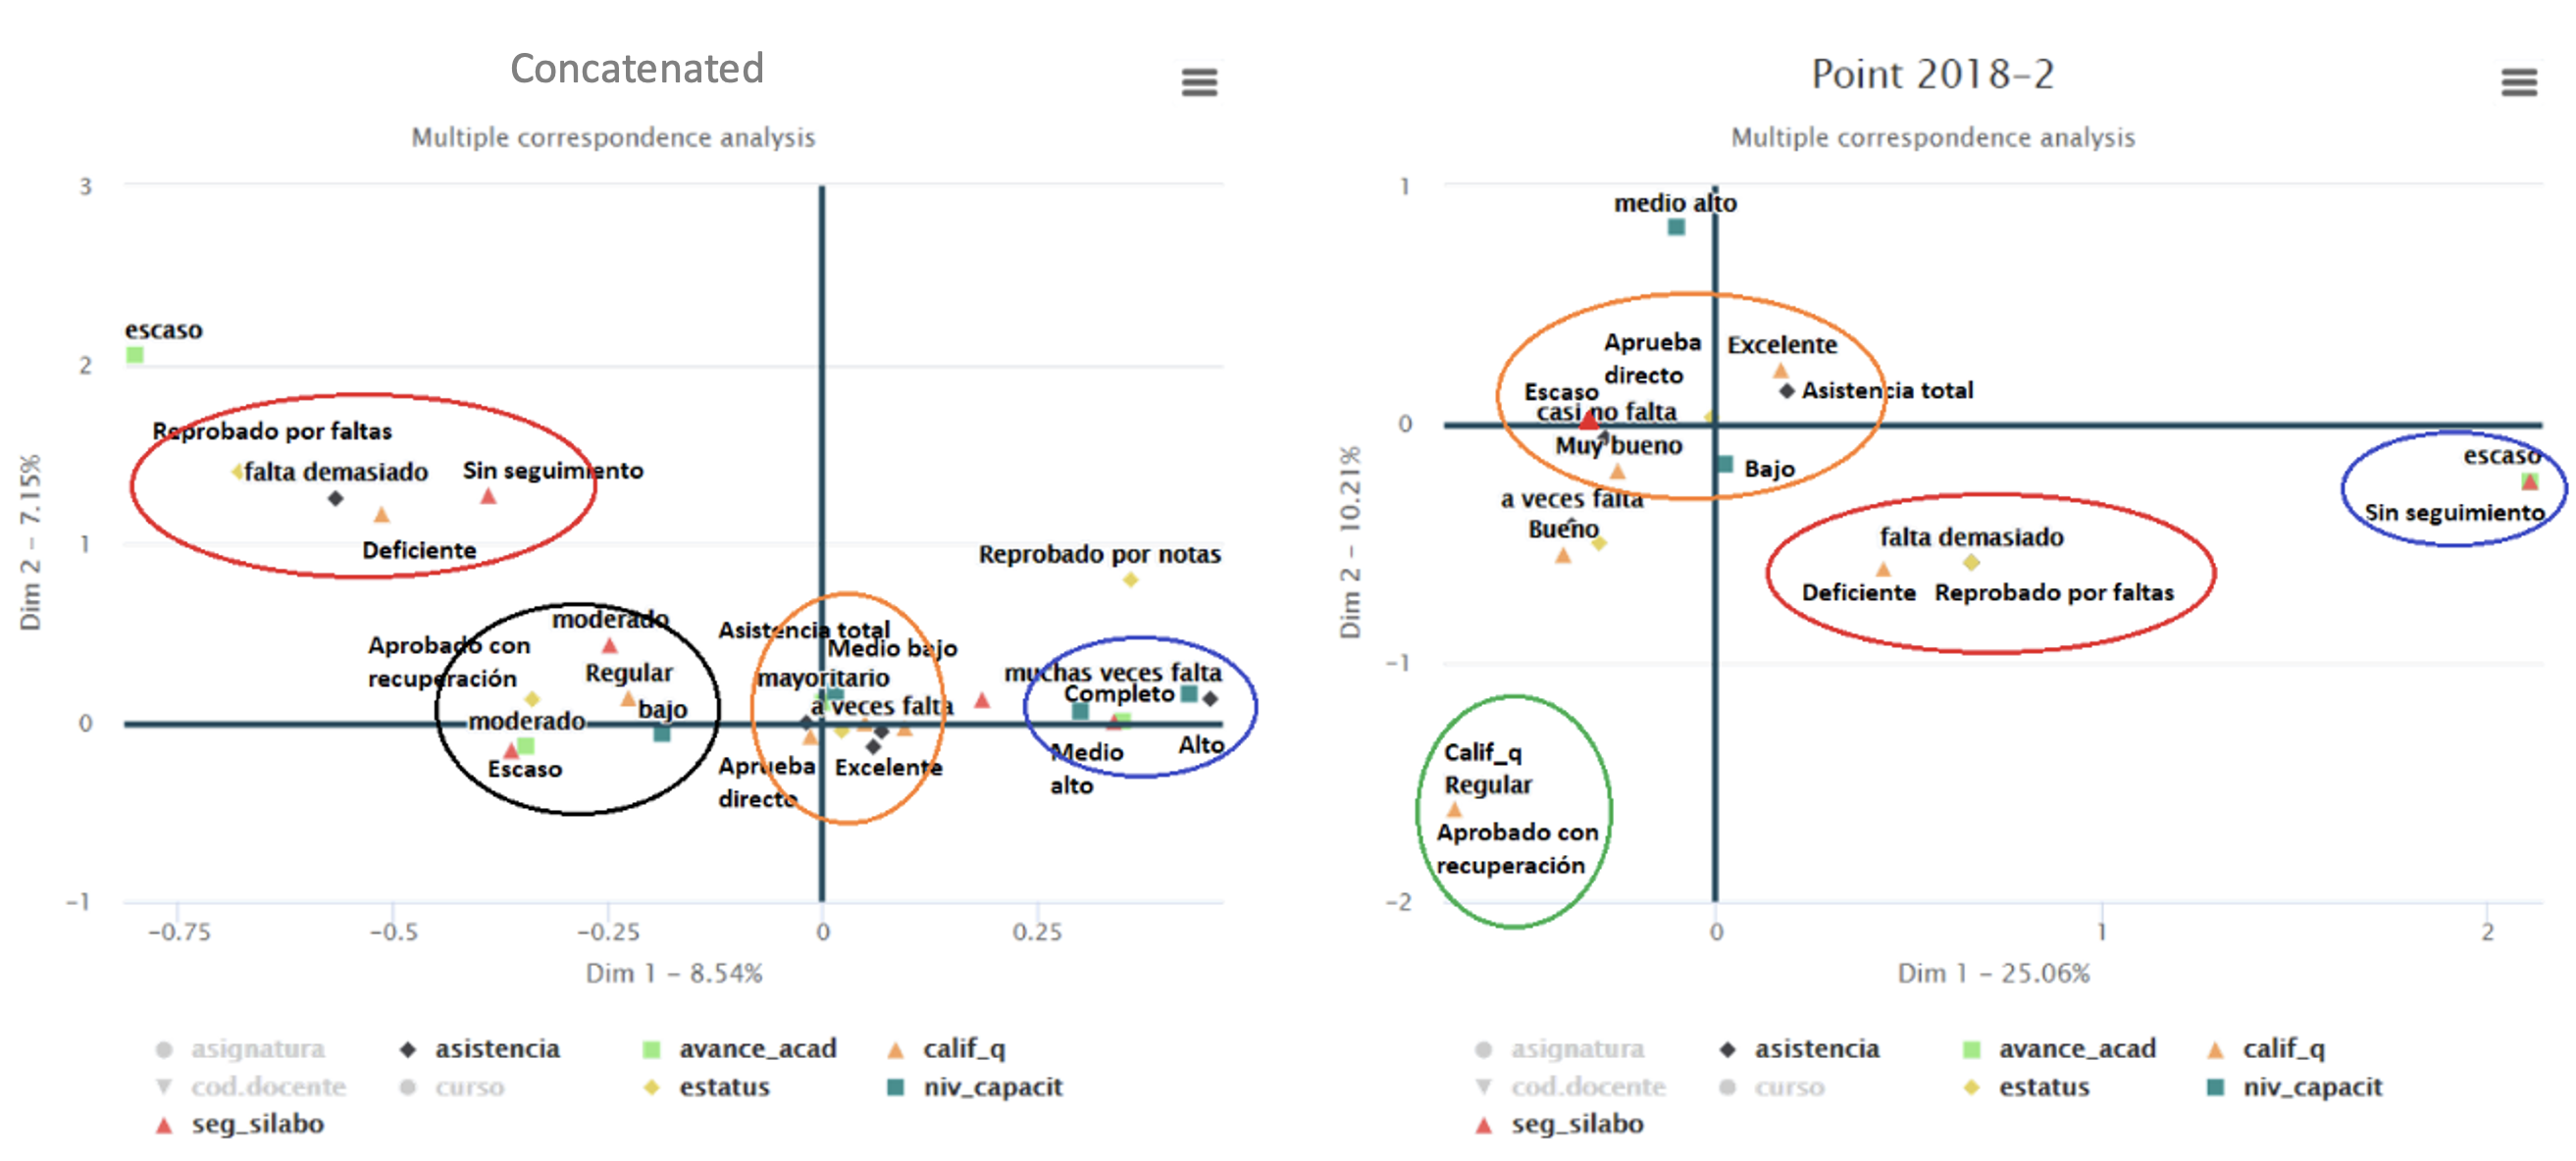
\includegraphics[width=0.9\linewidth,]{comp_edu} \end{center}

\caption{MCA de la tabla concatenada y 2018-2 con énfasis en los cambios en la asociación de categorías de las variables.}
\label{fig:compedu}
\end{figure}

En la figura \ref{fig:compedu} se observa cambios en la asociación de
las categorías de la variable Capacitación docente, en la tabla
concatenada el nivel más frecuente fue \emph{Medio bajo}, mientras que
en la 2018-2, fue \emph{Bajo.} Esto se explica porque la tabla
concatenada contiene información de todas las tablas, incluyendo la de
periodos académicos más recientes que enmascaran los datos de 2018-2. En
2018-2 el proceso de capacitación docente todavía se mostraba
incipiente, muchos profesores de la carrera no se capacitaban de forma
sistemática; las asignaturas que lograron avance académico
\emph{Completo} y cuyos estudiantes tuvieron \emph{Asistencia total},
rendimiento académico \emph{Muy bueno} y aprobaron de forma directa,
estuvieron a cargo de profesores con un \emph{Bajo nivel} de
capacitación. Con el paso del tiempo, la capacitación docente se fue
consolidando, en 2021-2, el periodo más reciente analizado en este
estudio, el nivel más frecuente ya subió a \emph{Medio alto}.

Otra variable que marcó una diferencia notoria fue Calificación. En el
gráfico de la tabla concatenada las tres categorías más altas de esta
variable estaban juntas y se asociaban con \emph{Aprueba directo} de la
variable Estatus. En la tabla 2018-2, ya no lucen juntas y más bien se
perfila una asociación con los niveles de la variable Asistencia. Los
estudiantes que tuvieron un 100\% de asistencia lograron calificaciones
de \emph{Excelente}, los que casi no faltaban a clases, de \emph{Muy
bueno}. Ambos grupos aprobaron las asignaturas de forma directa. Los que
a veces faltaban a clases tuvieron calificaciones equivalentes a
\emph{Bueno} y muchos reprobaron asignaturas por bajas notas. Los que
faltaban demasiado a clases reprobaron por faltas.

Estas categorías de variables que han cambiado su ubicación y su grado
de asociación de manera sensible pueden estar ocasionando el estado
fuera de control. La identificación de estas tablas se facilita cuando
se analiza la figura \ref{fig:chisqedu}.

\begin{figure}[H]


\begin{center}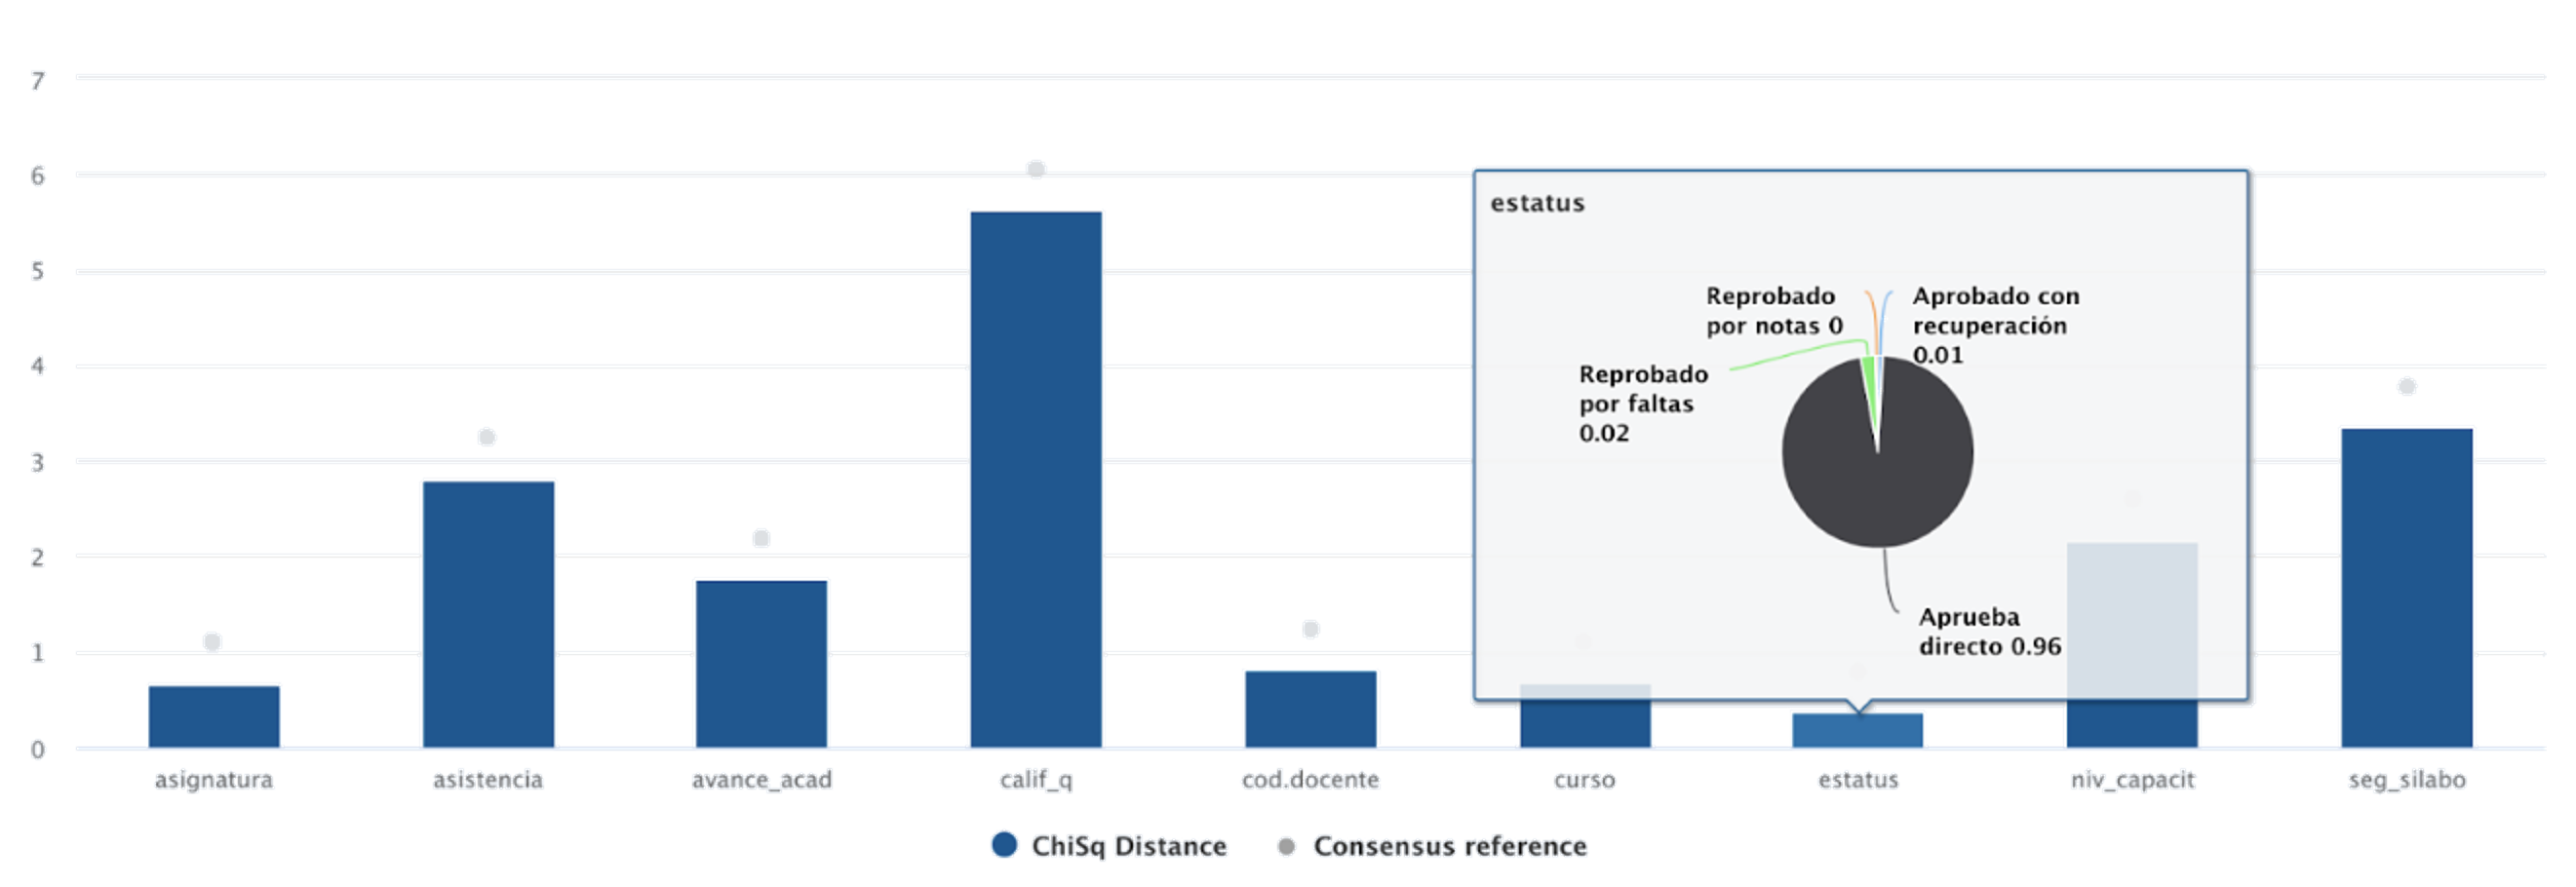
\includegraphics[width=0.9\linewidth,]{chisq_edu} \end{center}

\caption{Distancia $\chi^{2}$ entre las masas de la tabla concatenada y la 2018-2, $bd$ $pafd$.}
\label{fig:chisqedu}
\end{figure}

La figura \ref{fig:chisqedu}, permite apreciar, en un gráfico de barras,
la distancia Chi cuadrado entre las categorías de la tabla concatenada y
de la tabla 2018-2, reportada como fuera de control. Mientras más altas
son las barras, mayor es esta distancia. Estas variables son las que con
mayor fuerza están provocando el desplazamiento de la centralidad del
proceso y llevando al punto señalado a un estado fuera de control. En
consecuencia, es en ellas que se debe profundizar el análisis
comparativo mediante el MCA.

En la figura \ref{fig:chisqedu}, la barra más alta representa a las
calificaciones de los estudiantes, su análisis requiere la revisión de
la distribución de las categorías de la tabla Concatenada y la 2018-2,
que en el aplicativo T2Qv se realiza mediante la comparación de la
distribución de las categorías en los gráficos circulares de las tablas
analizadas, gráficos interactivos que aparecen al mover el cursor sobre
el gráfico de barras (figura \ref{fig:dist20182}).

\begin{figure}[H]


\begin{center}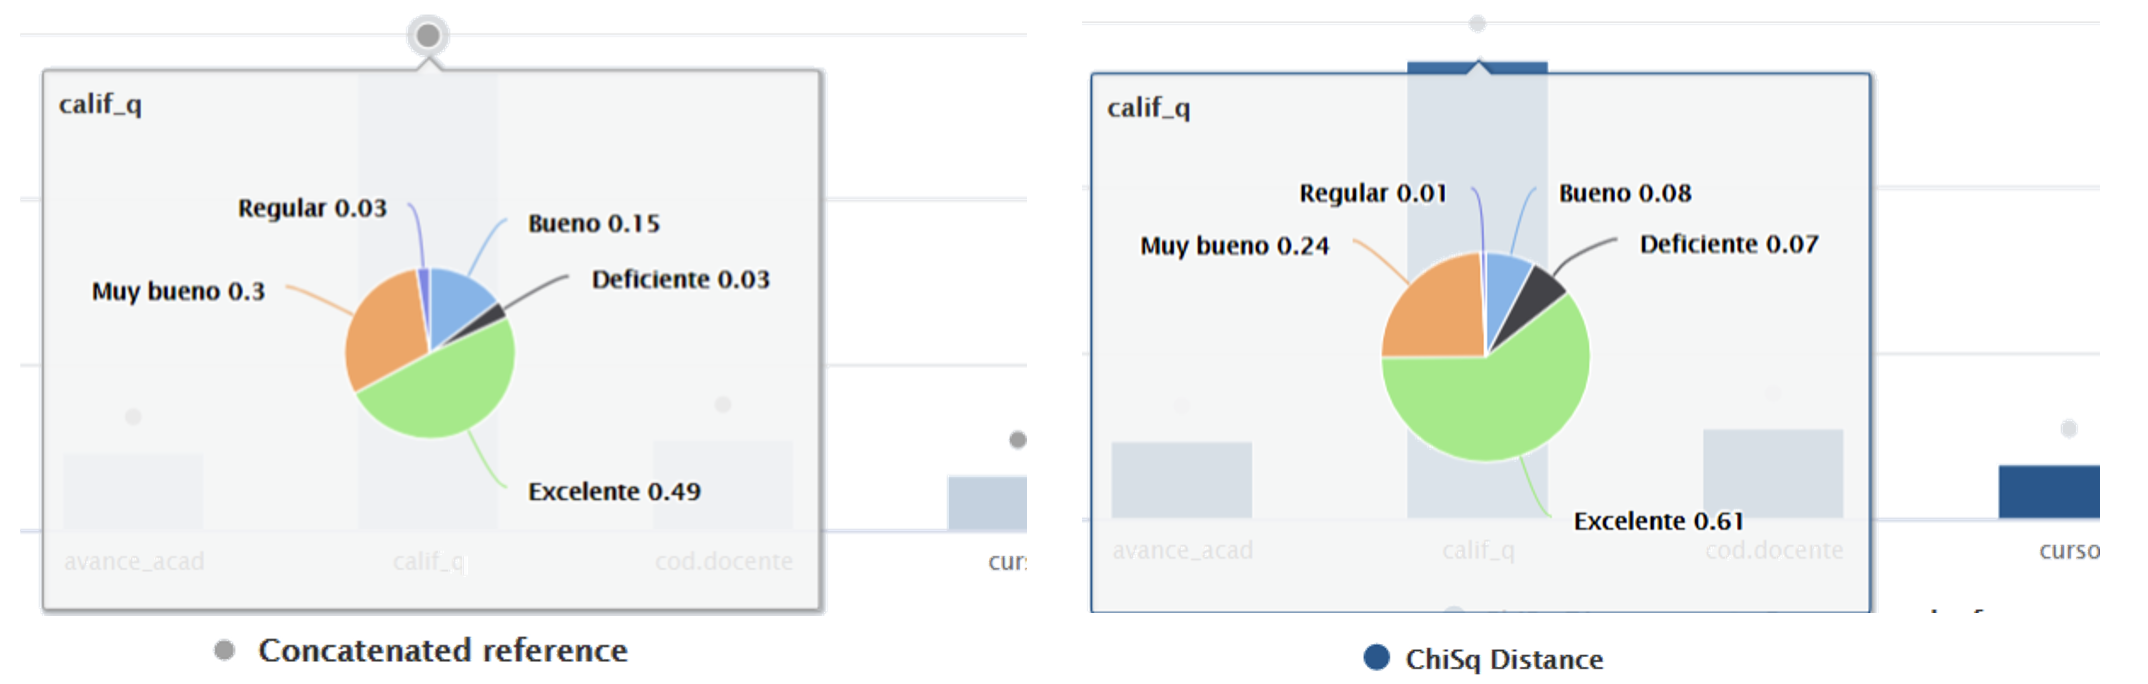
\includegraphics[width=0.9\linewidth,]{dist20182} \end{center}

\caption{Distribución de las categorías de la variable Calificación en la tabla Concatenada y la 2018-2 en el aplicativo T2Qv.}
\label{fig:dist20182}
\end{figure}

Al hacer la comparación se observa que en 2018-2, la categoría de
\emph{Excelente} tuvo mayores frecuencias relativas (0.61) que la
Concatenada (0.49); mientras que, en la categoría de \emph{Muy bueno},
la tabla 2018-2 tuvo una frecuencia relativa de 0.24 y la Concatenada
0.30. Se podría decir que el rendimiento académico en 2018-2 fue más
alto, posiblemente porque en ese periodo sólo había 25 asignaturas, de
un nivel básico y que corresponden a los primeros cuatro primeros
semestres que tenía la carrera en aquel momento. La tabla concatenada ya
registra la información de todas las 52 asignaturas en sus 8 semestres,
incluyendo las que se dirigen a profesionalización, a un mayor nivel de
complejidad.

Otra variable que demuestra alta incidencia en el desplazamiento de la
centralidad del proceso es Seguimiento al sílabo. Las categorías de esta
variable en la tabla consenso y la 2018-8 se observan en la figura
\ref{fig:dist2018n2}. Llama la atención que en 2018-2, la totalidad de
los casos reporten un nivel Escaso o de Sin seguimiento, no aparecen las
categorías Seguimiento Completo, Mayoritario ni Moderado, que sí tienen
frecuencias relativas en la tabla Concatenada. Se vislumbra que en el
periodo 2018-2 el seguimiento al sílabo era una debilidad, pero, con el
paso del tiempo se fue consolidando como proceso.

\begin{figure}[H]


\begin{center}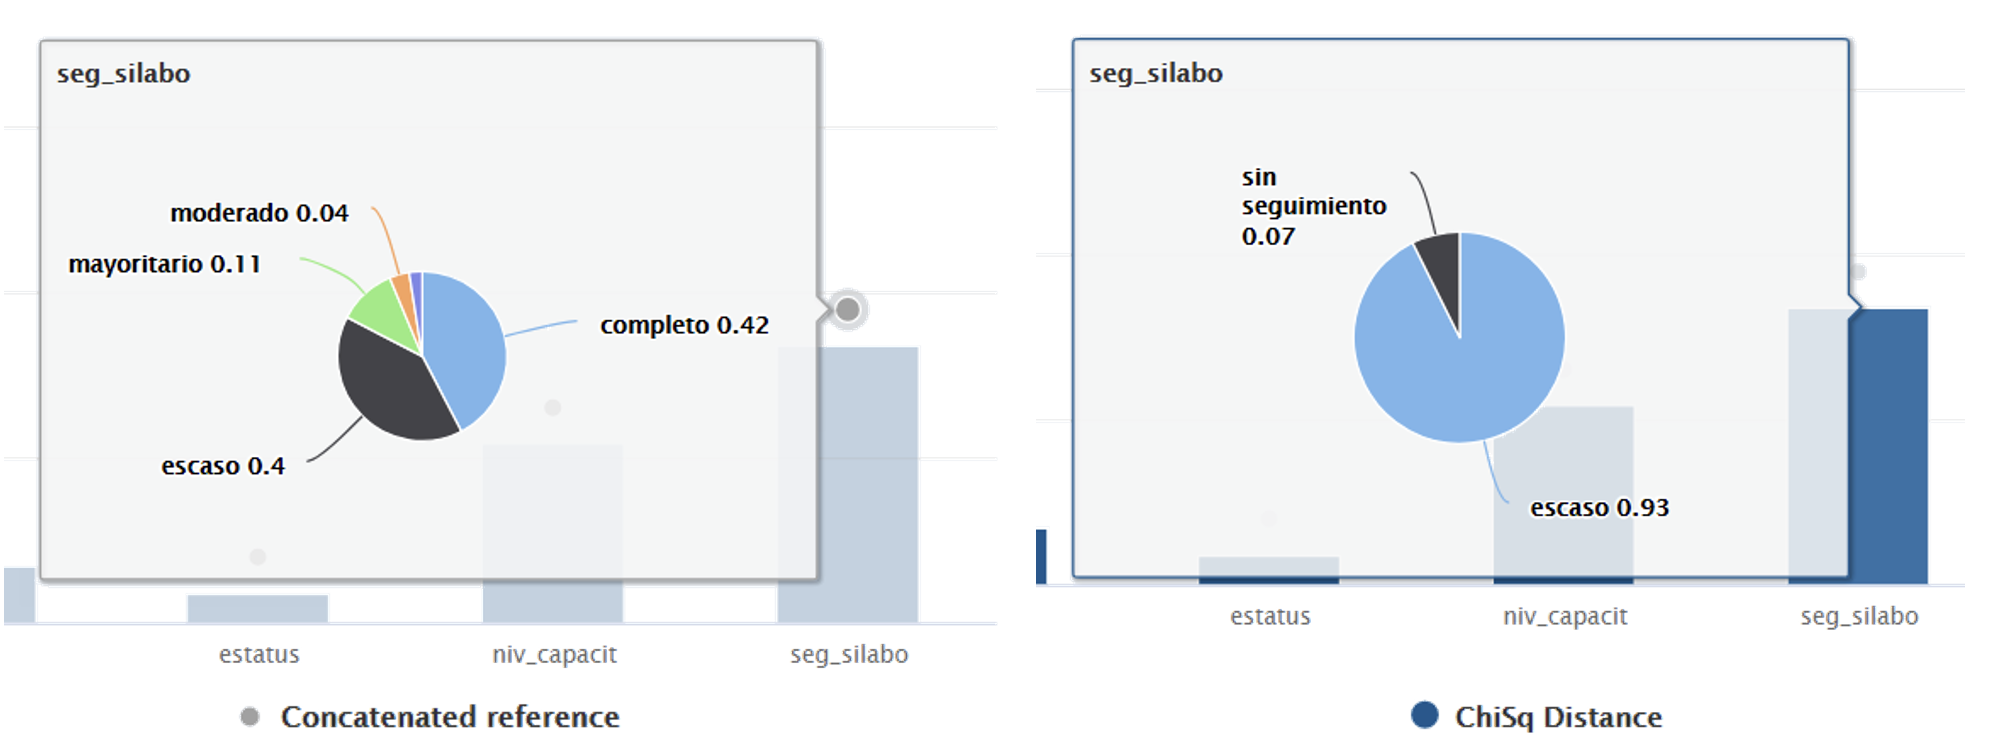
\includegraphics[width=0.9\linewidth,]{dist20182n1} \end{center}

\caption{Distribución de las categorías de la variable Seguimiento al sílabo en la tabla Concatenada y la 2018-2 en el aplicativo T2Qv.}
\label{fig:dist2018n1}
\end{figure}

Una tercera variable que participa en el desplazamiento de la
centralidad del proceso es el Nivel de Capacitación de los profesores.
La figura \ref{fig:dist20201n3} muestra la distribución de las
categorías en las tablas Concatenada y 2018-2. Se detecta que el proceso
de capacitación de los profesores no era una de las fortalezas de la
carrera en 2018-2, sin embargo, en la tabla concatenada, que incorpora
información de años más recientes, se observa una evolución del proceso
que de a poco se dirige hacia los niveles más altos.

\begin{figure}[H]


\begin{center}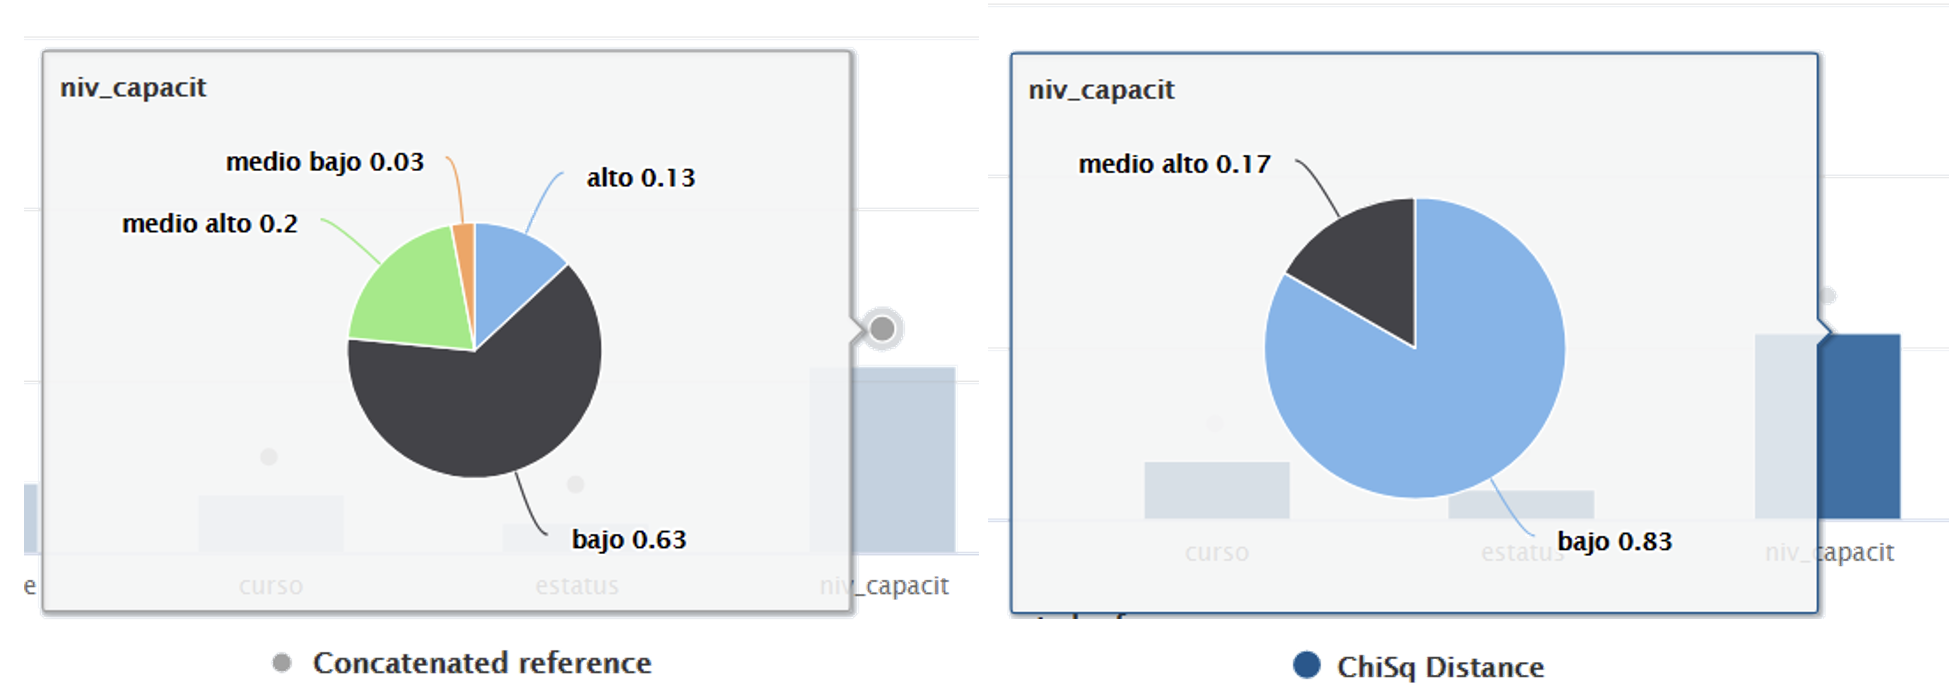
\includegraphics[width=0.9\linewidth,]{dist20182n2} \end{center}

\caption{Distribución de las categorías de la variable Nivel de capacitación en la tabla Concatenada y la 2018-2 en el aplicativo T2Qv.}
\label{fig:dist2018n2}
\end{figure}

Estos cambios en la distribución de las categorías de las variables
analizadas incrementan la variabilidad de la tabla 2018-2 y explican por
qué el proceso salió de control en este análisis de fase I.

La figura \ref{fig:point_2020_1} muestra el gráfico del MCA de la tabla
2020-1 y la figura 16, al de la tabla 2020-2. Ambas tablas fueron
reportadas en el gráfico T2 de Hotelling como fuera de control (figura
10), lo que sugiere afectaciones del proceso académico como consecuencia
de la implementación obligatoria de modalidad virtual debido a la
pandemia del COVID-19. No se puede negar esta afectación al proceso en
asignaturas como Fútbol sala, PEA natación, PEA baloncesto, Danza y
expresión corporal, entre otras, pero, más allá de detectar situaciones
generales externas que no se pueden cambiar, interesa determinar qué
variables que sí se pueden controlar salieron de control, lo que
ayudaría a tomar decisiones oportunas y corregir desviaciones. Esto se
analizará a continuación.

\begin{figure}[H]


\begin{center}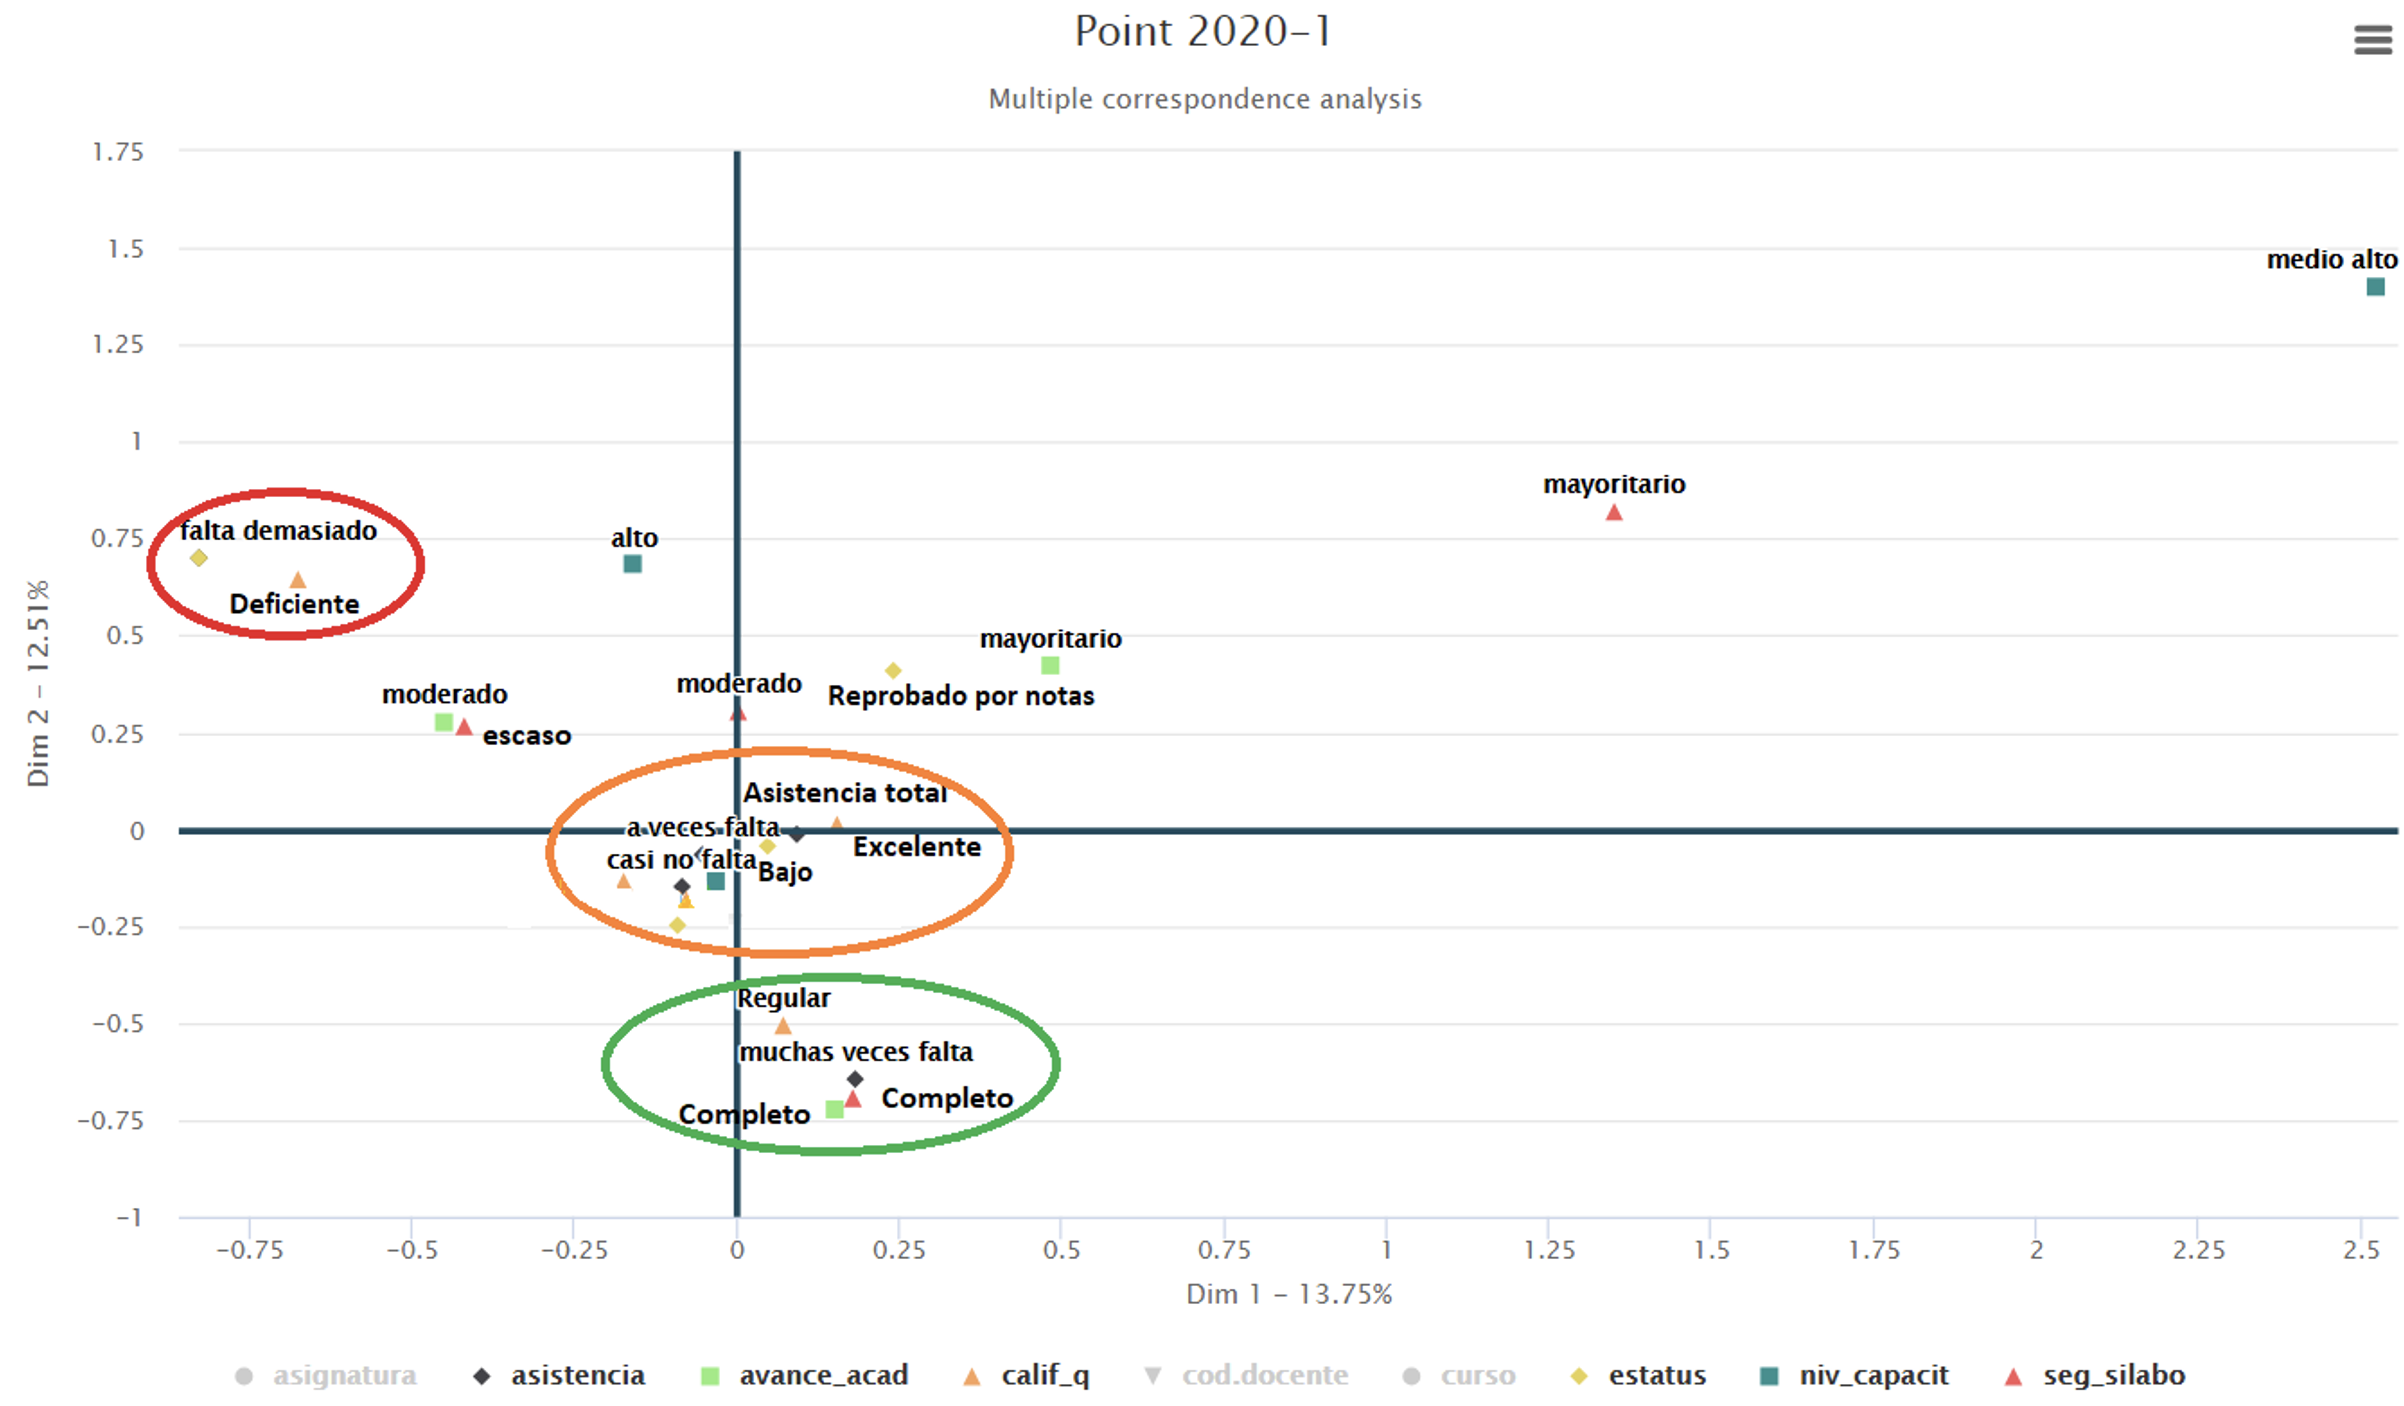
\includegraphics[width=0.9\linewidth,]{point_2020_1} \end{center}

\caption{Gráfico de MCA de la tabla 2020-1, $bd$ $pafd$.}
\label{fig:point_2020_1}
\end{figure}

La varianza explicada por el gráfico de la figura \ref{fig:point_2020_1}
es de 26.26\%. En la parte central se observan las categorías más
frecuentes que expresan una fuerte asociación entre los casos de
estudiantes que Aprueban directo las asignaturas con calificaciones de
\emph{Excelente}, niveles de inasistencia a clases bajos o nulos y un
nivel de capacitación de profesores \emph{Bajo.} La calificación de
\emph{Regular} se ha asociado a casos de estudiantes que \emph{muchas
veces faltan} a clases y la de \emph{Deficiente}, a estudiantes que
\emph{faltan demasiado} a clases.

El desarrollo completo de las actividades académicas planificadas,
reportado por el seguimiento al sílabo y el avance académico, no estuvo
asociado al mejor desempeño de los estudiantes, por el contrario, se
acercó más al rendimiento \emph{Regular.} Se interpreta que durante el
periodo 2020-1, en tiempos de pandemia y en modalidad de estudios
virtual, los aprendizajes necesitaron cierta flexibilidad académica por
parte de la carrera. El desarrollo completo del sílabo por parte de los
docentes tuvo especiales dificultades y la ejecución del seguimiento no
fue exactamente la prioridad para los estudiantes.

\begin{figure}[H]


\begin{center}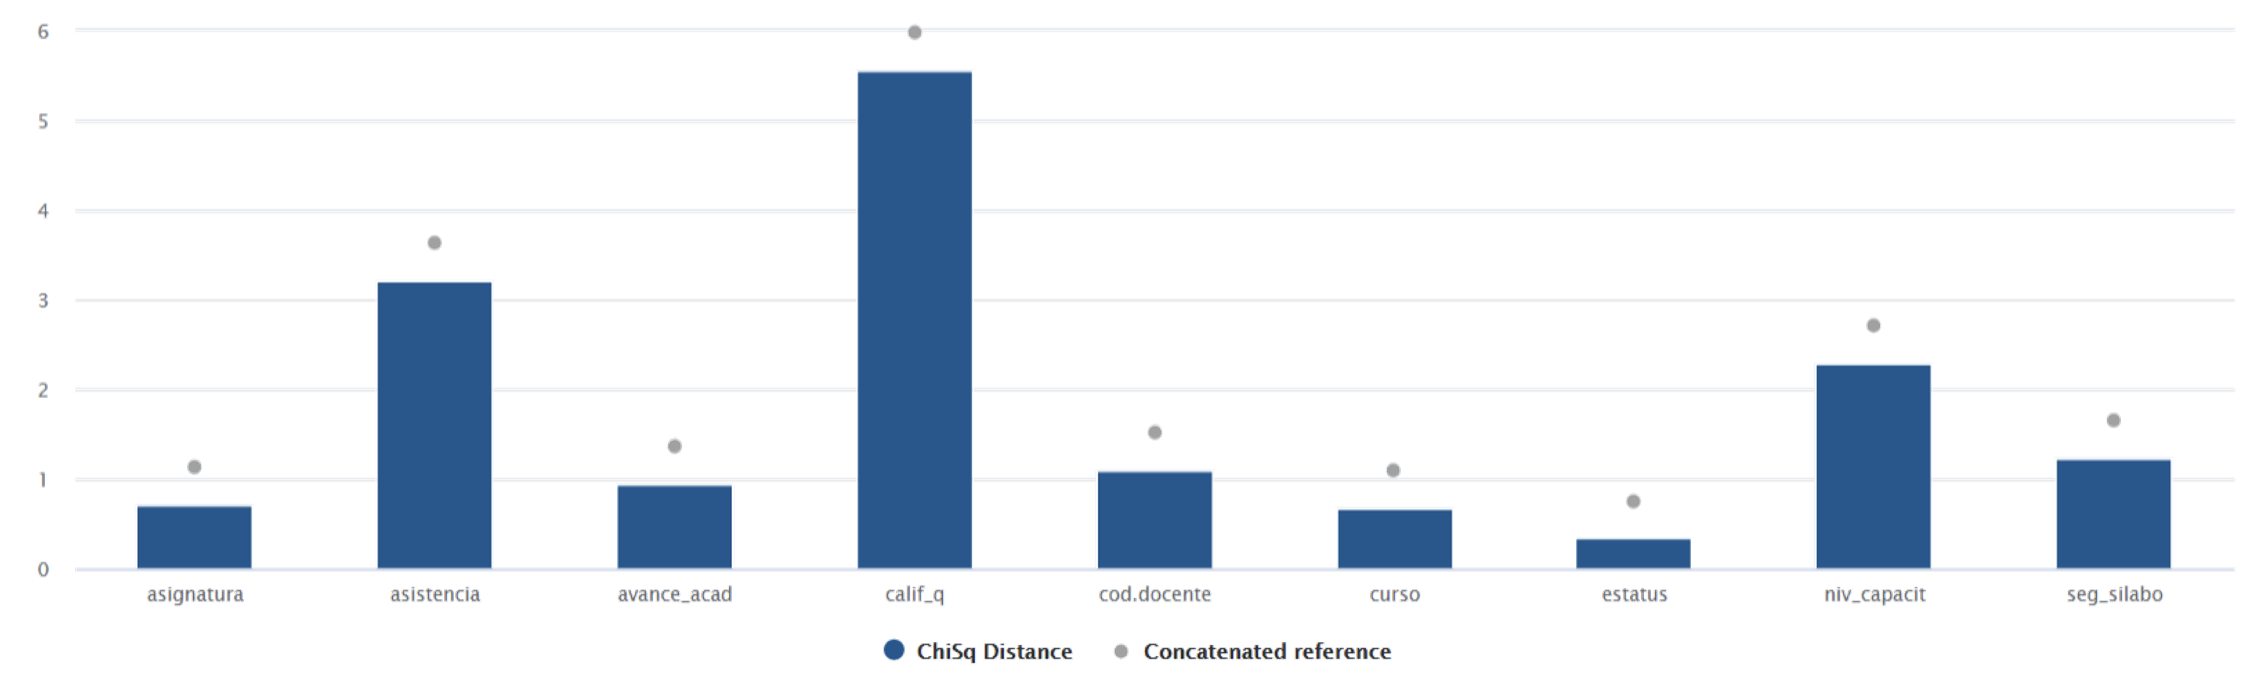
\includegraphics[width=0.9\linewidth,]{chisq_2020_1} \end{center}

\caption{Distancia $\chi^{2}$ entre las masas de la tabla concatenada y la 2020-1, $bd$ $pafd$.}
\label{fig:chi_2020_1}
\end{figure}

Para profundizar el análisis se revisa la figura \ref{fig:chi_2020_1},
que representa mediante un gráfico de barras la distancia \(\chi^2\)
entre las masas de la tabla 2020-1, reportada como fuera de control, y
la concatenada, tomada como referente. Las variables que más han
incidido en la salida de control son Calificación, Asistencia y Nivel de
capacitación. La figura \ref{fig:dist20201n3} permite comprobar la
variación de las frecuencias relativas de las categorías de estas
variables entre las tablas analizadas.

\begin{figure}[H]


\begin{center}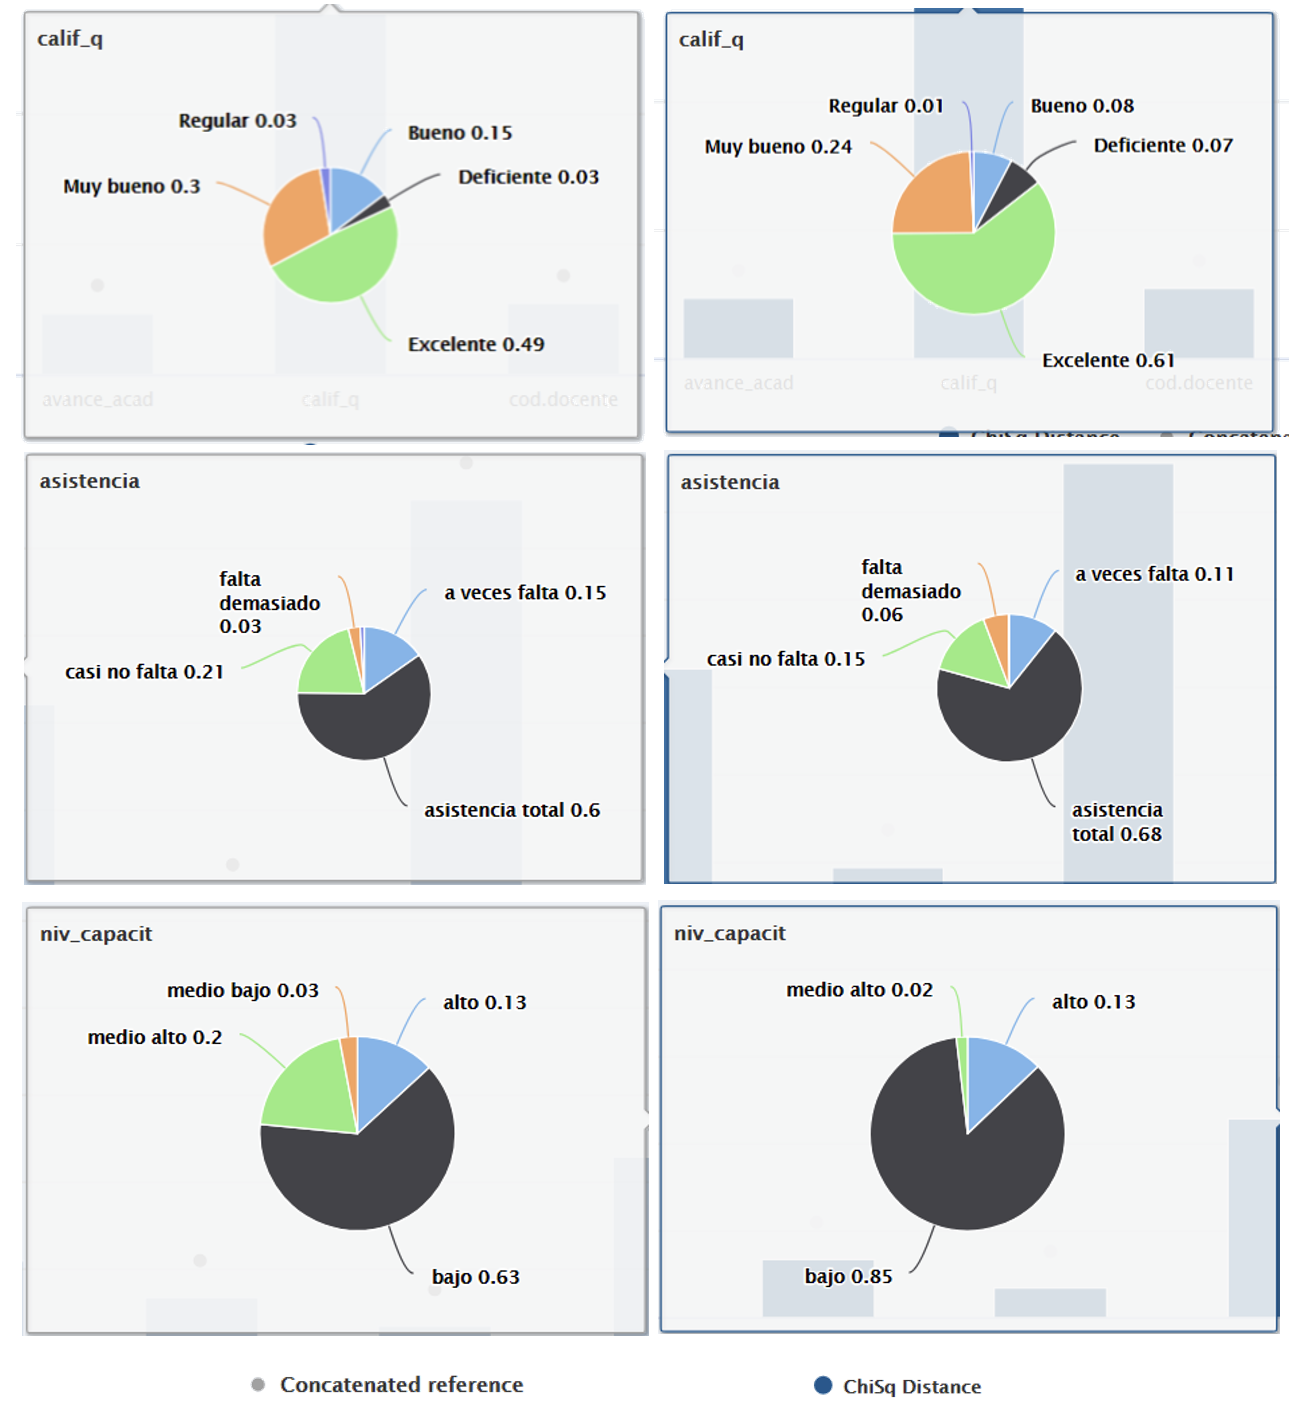
\includegraphics[width=0.9\linewidth,]{dist20201n3} \end{center}

\caption{Distribución de las categorías de las variables Calificación, Asistencia y Nivel de capacitación en la tabla Concatenada y la 2020-1 en el aplicativo T2Qv.}
\label{fig:dist20201n3}
\end{figure}

De la lectura de la figura \ref{fig:dist20201n3} se interpreta que el
rendimiento académico en 2020-1 fue más alto que el reportado por la
tabla Concatenada, pero no tanto como en la 2018-2, de todos modos, tuvo
incidencia en la variación de la tendencia central el proceso. Por otra
parte, en ambas tablas la asistencia a clases no es un problema, más del
80\% de casos demuestran \emph{asistencia total} o que los estudiantes
\emph{casi no faltan} a clases, esto tiene especial valor en época de
pandemia. Las diferencias se dirigen a distribución interna de las
categorías, así, las frecuencias relativas de \emph{Asistencia total} en
la tabla Concatenada tienen un valor de 60\% y en la 2020-1, de 68\%;
las frecuencias de \emph{Casi no falta} están en 21\% y 15\%,
respectivamente.

En ambas tablas, la clase \emph{Bajo} de la variable Nivel de
capacitación es predominante, 63\% en la tabla Concatenada y 85\% en la
2020-1. Sin embargo, esta variable presenta marcadas diferencias en la
estructura interna de las dos tablas comparadas. El nivel \emph{Medio
alto} tiene una frecuencia bastante mayor en la tabla Concatenada (20\%)
que en la 2020-1 (2\%), el nivel Medio bajo está ausente en la 2020-1.
La lectura de esta información sugiere que la capacitación docente, una
de las variables más importantes para el desarrollo eficaz del proceso
académico, aunque ha ido mejorando de a poco, en 2020-1 todavía no
adquiría su verdadera relevancia entre el personal docente, peor aún, en
época de pandemia.

\begin{figure}[H]


\begin{center}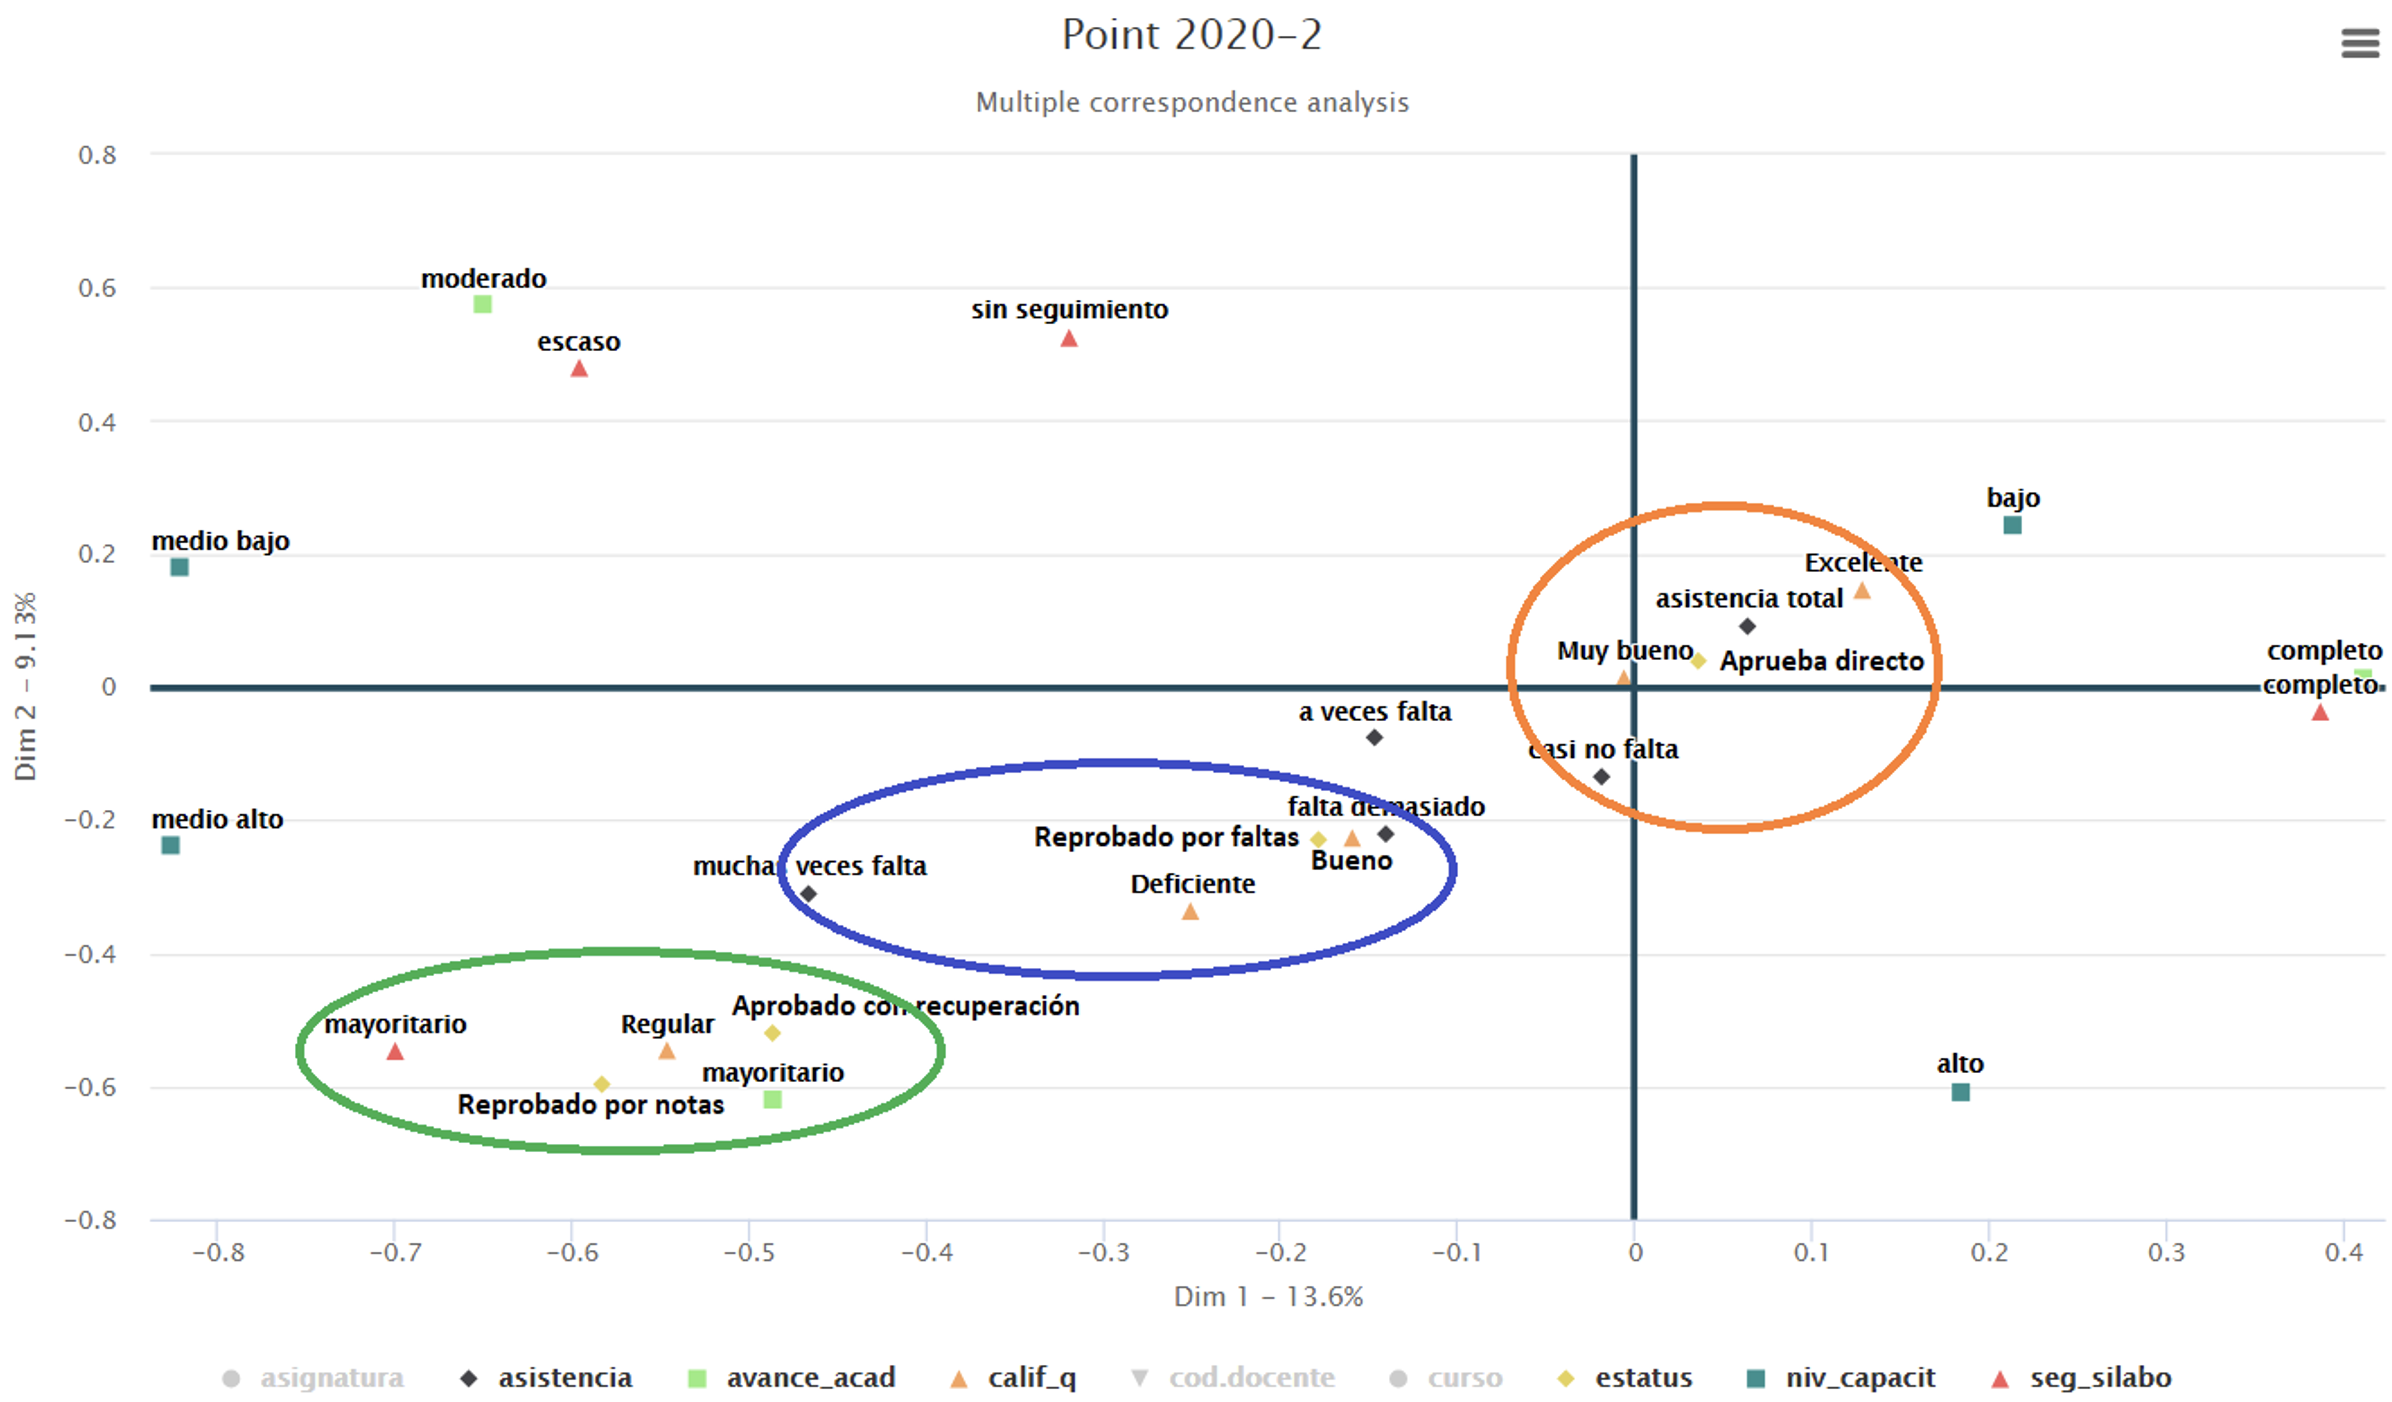
\includegraphics[width=0.9\linewidth,]{point_2022_2} \end{center}

\caption{Gráfico de MCA de la tabla 2020-2, $bd$ $pafd$.}
\label{fig:point_2022_2}
\end{figure}

La figura \ref{fig:point_2022_2} permite observar el gráfico del MCA de
la tabla 2020-2. Con una varianza acumulada de 22.72\%.

En este periodo, las calificaciones más frecuentes son las de
\emph{Excelente} y \emph{Muy bueno}, que de forma conjunta llegan a
representar un 76.5\% del total de casos. Estos altos niveles de
calificación se asocian a grupos de estudiantes que mantuvieron alta
asistencia a clases y, en consecuencia, aprobaron de forma directa las
asignaturas (91.5\%). Las calificaciones de \emph{Bueno} y
\emph{Deficiente} se asocian a estudiantes que han tenido inconvenientes
por reiterada inasistencia a clases, de manera que en un 3.0\% de los
casos reprobaron asignaturas por faltas.

Se observa también un grupo minoritario (4.0\%) con calificaciones de
\emph{Regular}, que se ha asociado con estudiantes que acudieron a
exámenes de recuperación para aprobar sus asignaturas (4.5\%) y con
otros que al final las reprobaron por bajas calificaciones (3.0\%). En
este grupo se manifiesta también asociación con la categoría
\emph{Mayoritario} en las variables Seguimiento al sílabo y Avance
académico. A diferencia de la tabla concatenada, el mayor avance
académico en el periodo 2020-2 se corresponde con los mejores resultados
académicos expresados en los grupos de calificaciones de
\emph{Excelente} y \emph{Muy bueno}.

\begin{figure}[H]


\begin{center}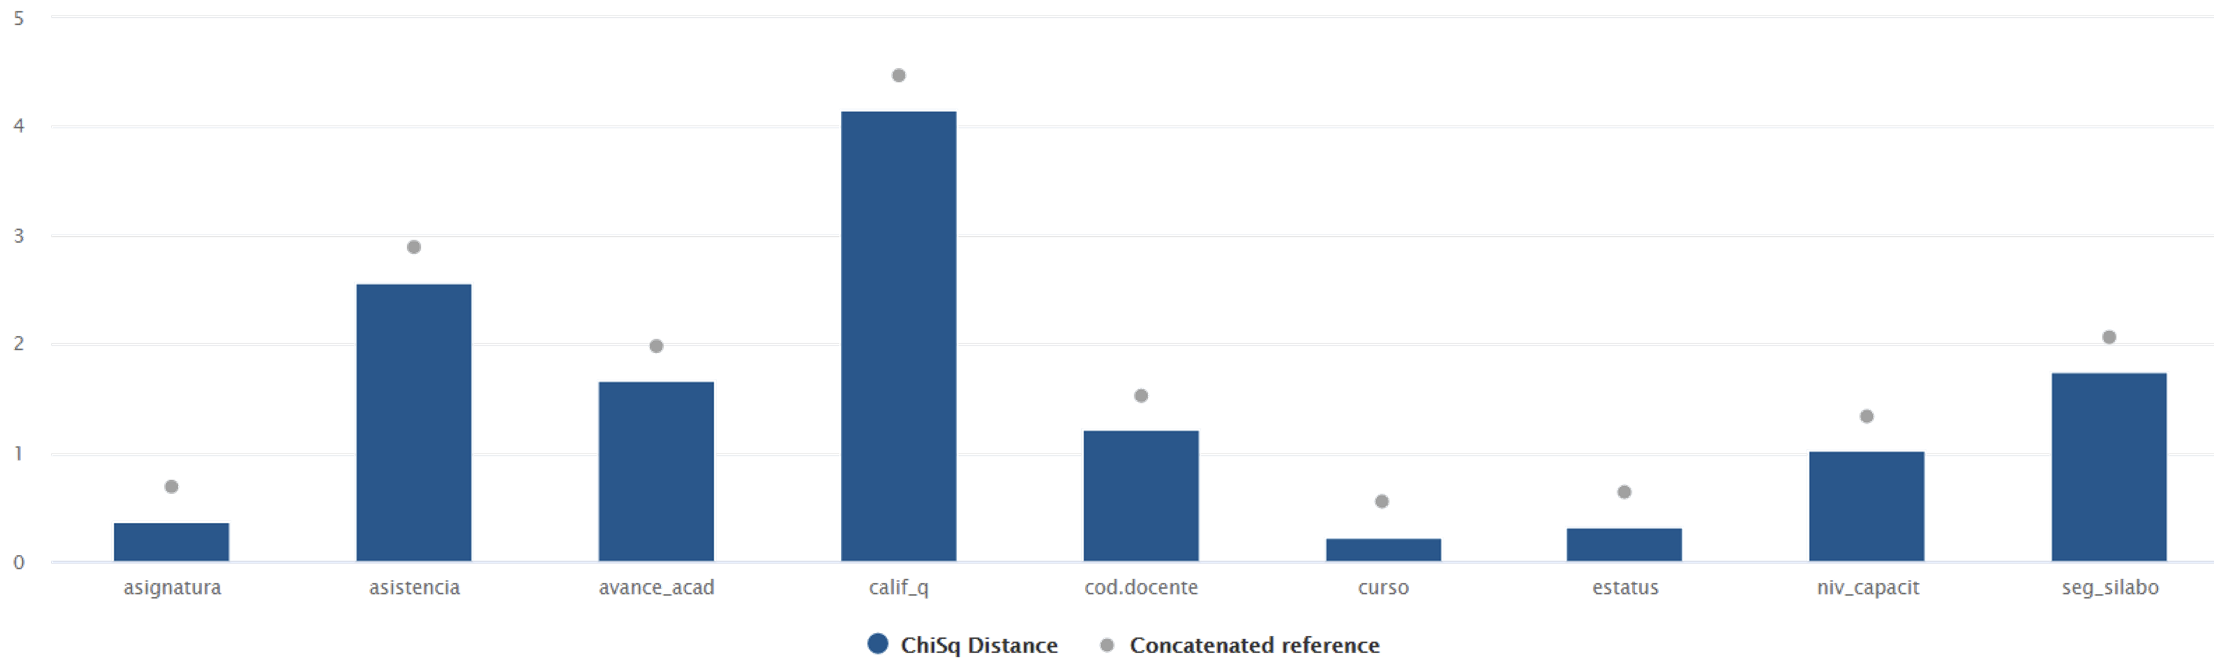
\includegraphics[width=0.9\linewidth,]{chi20202n5} \end{center}

\caption{Distancia $\chi^2$ entre las masas de la tabla consenso y la 2020-2, $bd$ $pafd$.}
\label{fig:chi20202n5}
\end{figure}

Como se observa en la figura \ref{fig:chi20202n5}, las mayores
distancias \(\chi^2\) entre las masas de la tabla consenso y la 2020-2
están dados por las variables Calificación, Asistencia y Seguimiento al
sílabo. La distribución interna de las categorías de estas variables se
registra en la figura \ref{fig:dist20202n6}.

\begin{figure}[H]


\begin{center}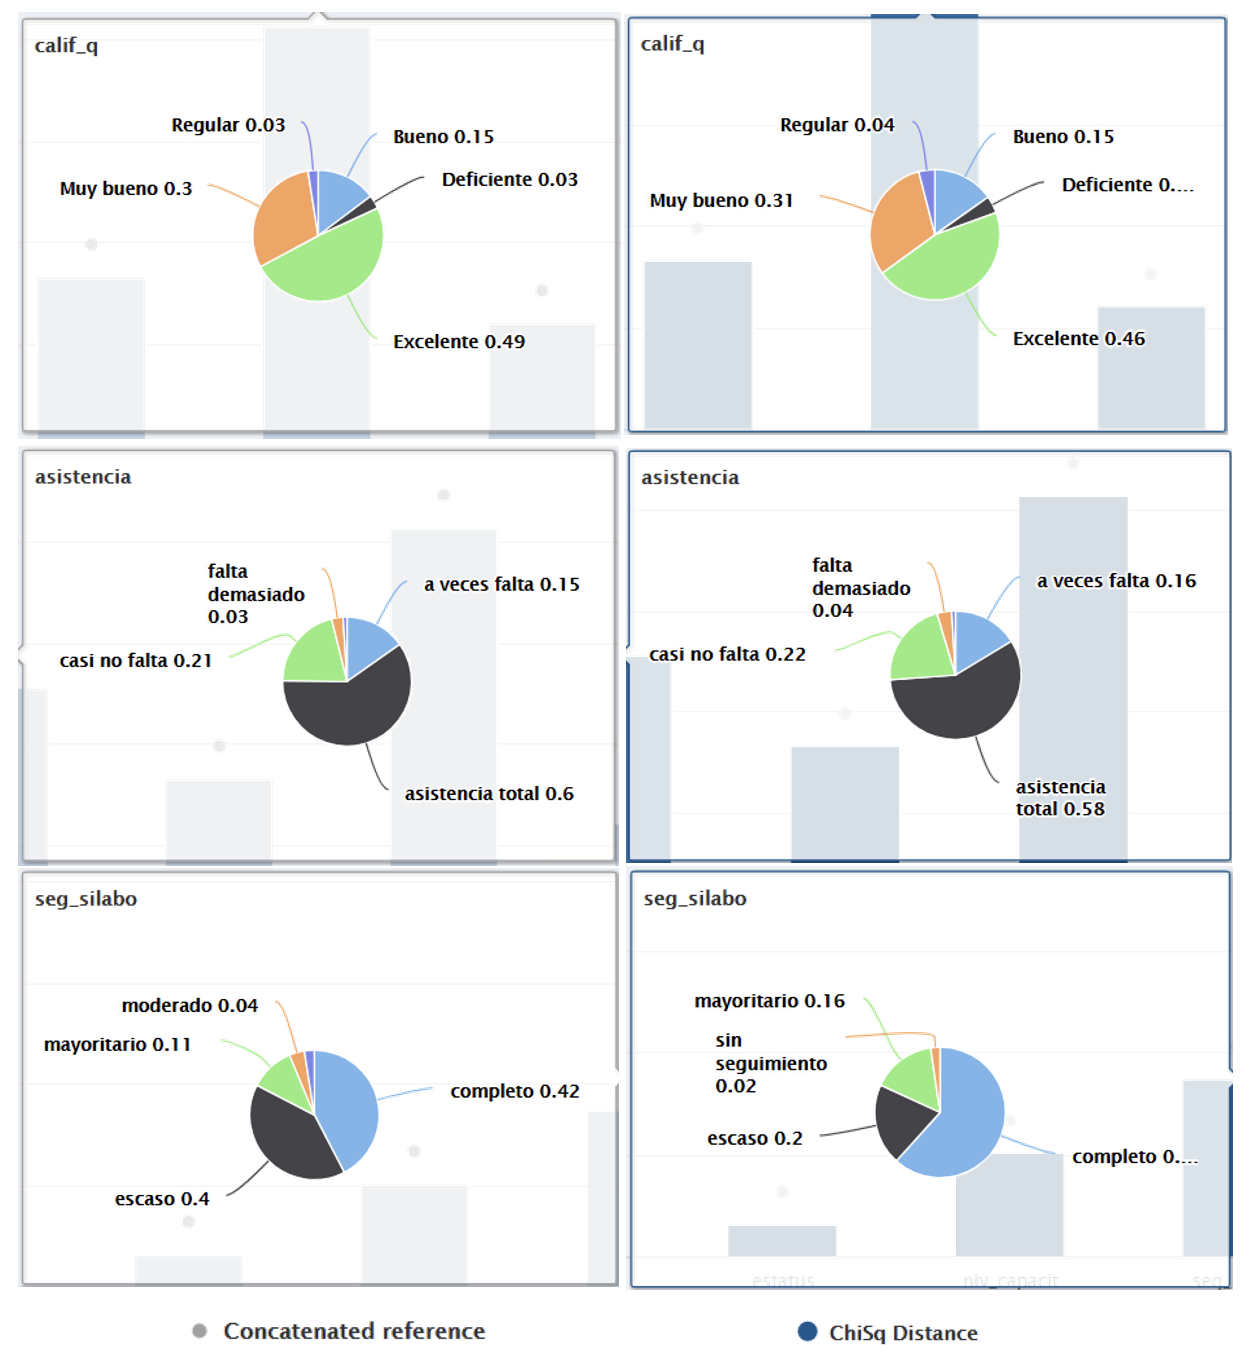
\includegraphics[width=0.9\linewidth,]{dist20202n6} \end{center}

\caption{Distribución de las categorías de las variables Calificación, Asistencia y Seguimiento al sílabo en la tabla Concatenada y la 2020-2 en el aplicativo T2Qv.}
\label{fig:dist20202n6}
\end{figure}

La distribución interna de las variables Calificaciones y Asistencia no
es muy distinta en la tabla Concatenada y la 2020-1, se observa pequeñas
diferencias que, en la práctica, sugieren que el comportamiento de ambas
variables es semejante en ambas tablas comparadas.

No sucede lo mismo con la variable Seguimiento al sílabo, allí sí es
evidente la diferencia. La categoría de seguimiento \emph{Completo}, en
la tabla 2020-2, tiene una frecuencia relativa de 0.62, mientras que en
la concatenada tiene 0.42. Otra categoría que muestra amplia diferencia
es \emph{Escaso}, en la tabla 2020-1 reporta un valor de 0.20, mientras
que en la Concatenada, 0.40. Además, la categoría \emph{Moderado}, que
en la tabla concatenada alcanza un valor de 0.04, no aparece en la
2020-1.

Se ha analizado la estructura interna de las variables que han tenido
alta incidencia en el desplazamiento de la tendencia central del proceso
analizado, sin embargo, es importante destacar que la salida de control
no se puede atribuir a la acción individual de una variable, o a la
acción por separado de un grupo de variables, sino al efecto combinado
de variables correlacionadas. Todas las variables contribuyen en mayor o
menor medida a explicar el comportamiento del proceso, por esa razón es
preciso realizar este análisis estadístico multivariante.

\hypertarget{anuxe1lisis-de-sensibilidad}{%
\section{Análisis de sensibilidad}\label{anuxe1lisis-de-sensibilidad}}

Como se ha mencionado, en el gráfico T2Qv un punto fuera de control se
interpreta como una tabla (\(k_i\)) que incluye una cantidad o una
proporción de variables contaminadas. En estos casos, se espera que los
puntos en el gráfico T2Qv generalicen el comportamiento de estas
diferencias en su distribución y así se supere el límite de control
superior (UCL). La ubicación de este límite de control varía en función
del número de dimensiones que se representen, así, cuando es alto se
logra un desempeño óptimo, mientras que, se introduce inestabilidad y se
pierde confiabilidad en los resultados al disminuir el número de
dimensiones que se pueden representar.

El gráfico de control propuesto es capaz de detectar un punto fuera de
control, aún con un bajo número de variables contaminadas, cuando se
trabaja con un alto número de dimensiones. Se recomienda \(p - 1\), tal
que \emph{p} es el número total de dimensiones de la matriz inicial
(Tabla \ref{tab:inicial}). Cuando se disminuye el número de dimensiones
también disminuye la altura del límite de control superior (UCL), en
consecuencia, se incrementa el número de puntos fuera de control, aunque
no necesariamente las variables expresen diferencias significativas en
su valores, crece la probabilidad de obtener error tipo I.

Por consiguiente, la pregunta que surge es hasta cuántas dimensiones se
puede disminuir en el análisis sin perder confiabilidad en el resultado.
La importancia de esta pregunta radica en la necesidad de disponer un
gráfico confiable, que identifique puntos fuera de control aún si se ha
aplicado a los datos una técnica de una reducción de dimensiones, sin
caer en casos de falso positivo.

\begin{figure}[H]


\begin{center}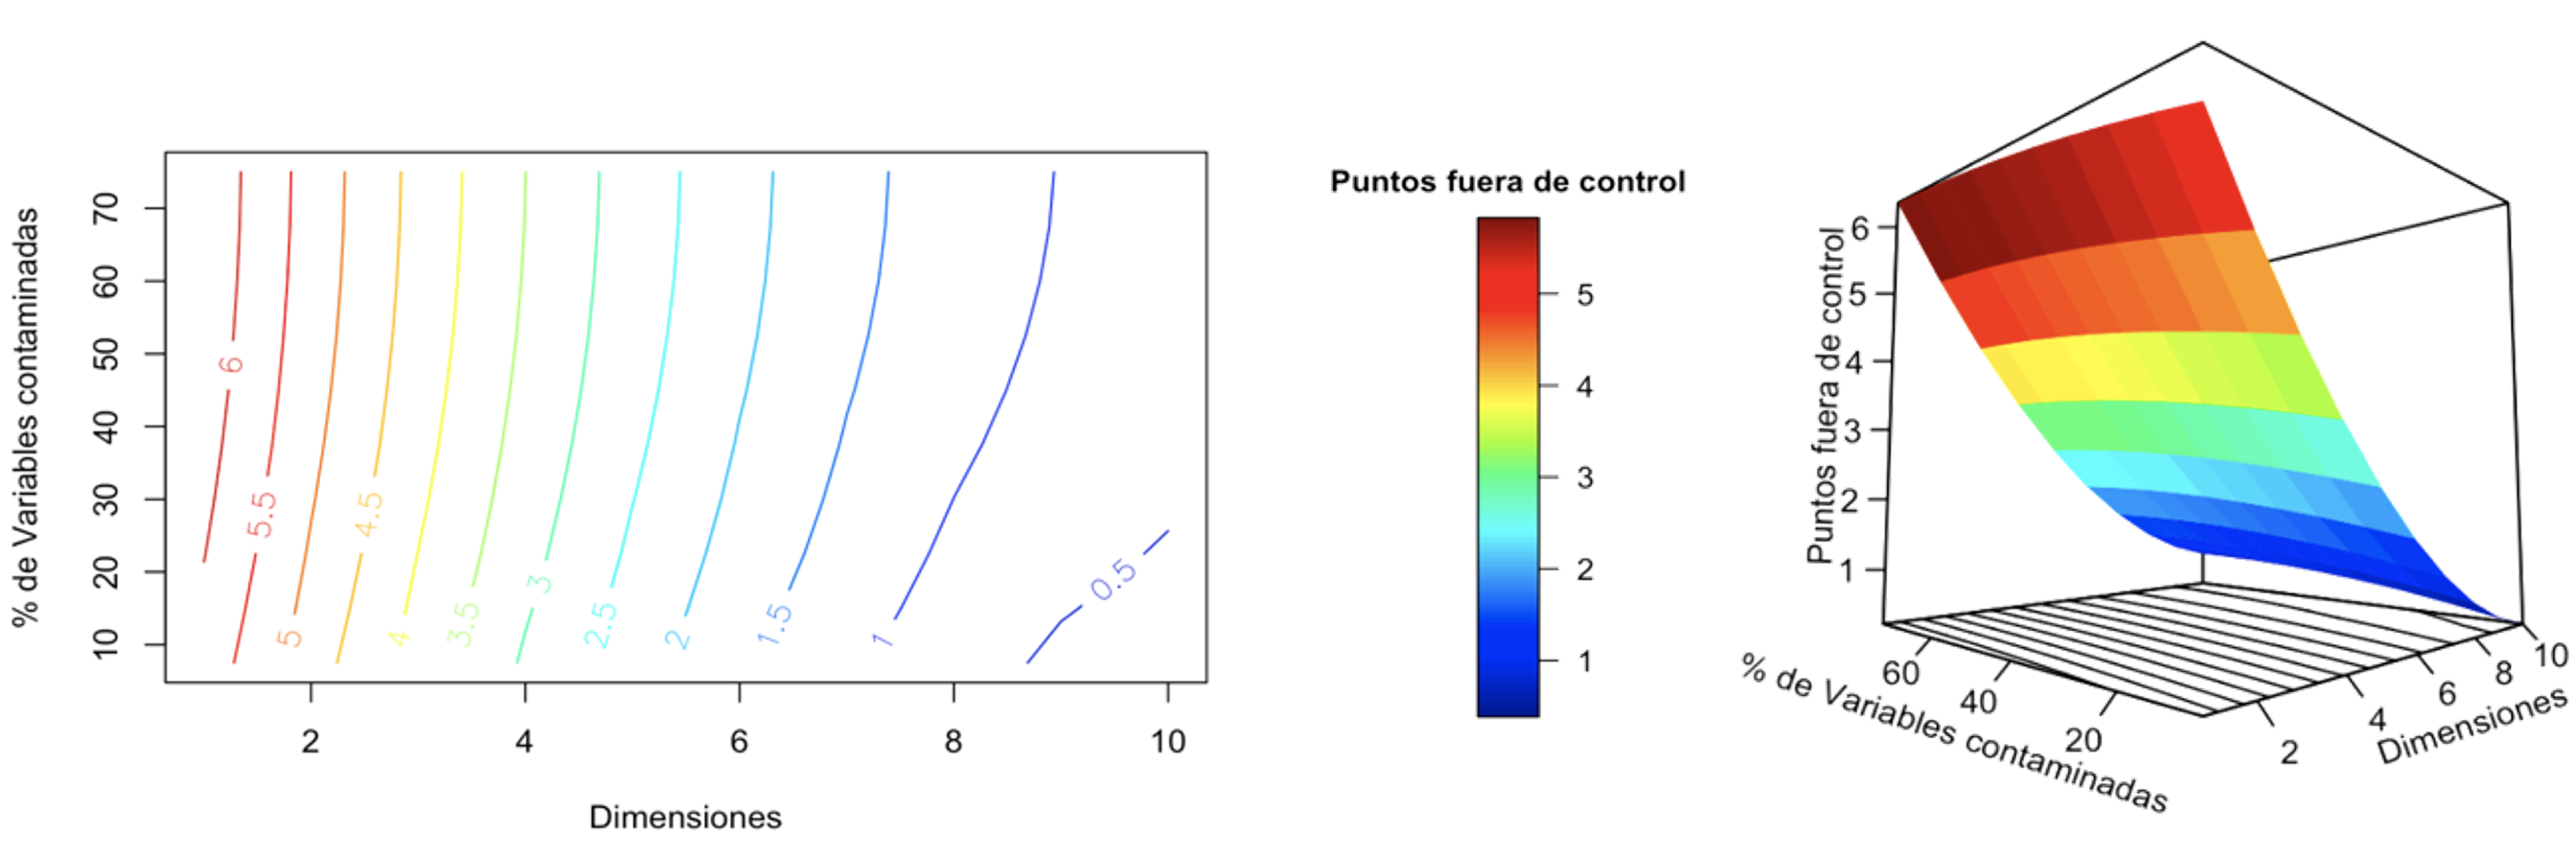
\includegraphics[width=0.9\linewidth,]{sensibilidad} \end{center}

\caption{Curvas de nivel y superficie de respuesta obtenidas con el gráfico T2Qv.}
\label{fig:sensibilidad}
\end{figure}

El análisis de sensibilidad utiliza curvas de nivel y superficies de
respuesta (figura \ref{fig:sensibilidad}) para representar el número de
puntos fuera de control, considerando el porcentaje de variables
contaminadas de la \emph{ki} tabla y el número de dimensiones
representadas. Los datos de prueba utilizados en el modelo se registran
en 10 tablas, cada una de ellas incluye 10 variables y cada variable
tiene tres categorías: \emph{alto, medio} y \emph{bajo.} La tabla 10
tiene una distribución diferente de las demás, esta es la tabla
contaminada.

Se observa que el modelo es capaz de identificar un punto fuera de
control trabajando con 9 dimensiones \emph{(p - 1)}, aún con un
porcentaje bajo de variables contaminadas. Cuando el número de
dimensiones disminuye a 8 y el porcentaje de variables contaminadas es
cercano a 100\%, detecta correctamente 1 punto fuera de control. Se
observa además que cuando el número de dimensiones es menor se pierde
estabilidad y se mitiga la potencia de la prueba. En consecuencia, el
análisis de sensibilidad ratifica que el gráfico de control T2Qv tiene
un buen rendimiento cuando trabaja con altas dimensiones.

\hypertarget{discusiuxf3n}{%
\section{Discusión}\label{discusiuxf3n}}

En el control estadístico de procesos todavía no son muchas las
propuestas publicadas sobre gráficos de control para variables
cualitativas. Las diferencias entre procedimientos para la determinación
de los estadísticos y los gráficos de control en este campo hacen
difícil su comparación. El gráfico de control T2Qv, que se presenta en
este artículo, aplica un MCA, técnica de análisis multivariante que
identifica estructuras latentes que subyacen en el conjunto de datos
cualitativos y que involucra una reducción de dimensiones, en
consecuencia, desde el comienzo se requiere una tabla de datos con
\emph{p} variables (\emph{p} \textgreater{} 3) dicotómicas o
politómicas. Se debe recordar que el análisis de sensibilidad determinó
que esta propuesta tiene un buen rendimiento cuando trabaja con altas
dimensiones y que a bajas dimensiones pierde estabilidad. En varios
estudios revisados, los casos de aplicación analizan sólo dos o tres
variables, lo que conduciría a la aplicación de un análisis de
correspondencias simple, no múltiple. En consecuencia, estos casos no
podrían ser tratados con el T2Qv.

Como ejemplos se señala la Combinación lineal óptima de variables
Poisson para el SPC multivariados, de \citet{epprecht2013optimal}, cuyo
caso de aplicación registrado en su publicación analiza dos variables
relacionadas con el conteo de defectos en la producción de jarrones de
cerámica. El gráfico GMDS de \citet{raza2019design} fue ejemplificado
con un conjunto de datos de telecomunicaciones, tomado de
\citet{jiang2002process}, que consta de sólo dos variables. El gráfico
de control multivariante, desarrollado por
\citet{pastuizaca2015multivariate}, para \emph{p} características de
calidad de atributos correlacionadas, que aplica teoría difusa, hace un
análisis de dos tablas tomadas de publicaciones de
\citet{taleb2009control} y \citet{taleb2006multivariate}, la primera con
tres variables relacionadas con la comida congelada, y la segunda, con
tres variables sobre la producción de porcelana.

Otra de las características del gráfico T2Qv es que cada muestra es un
grupo constituido por un conjunto de individuos. El ejemplo de datos
simulados \emph{Datak10Contaminated} incluye un conjunto de 10 tablas y
11 variables, cada tabla es una muestra, está formada por 100
observaciones y aparece representada como un punto en el gráfico T2 de
Hotelling; el ejemplo aplicado al contexto educativo hace referencia a
la base de datos \emph{bd\_pafd}, conformada por 8996 observaciones y 10
variables cualitativas agrupadas en 7 periodos académicos, estos
periodos constituyen las tablas (muestras) que se representan como
puntos en el gráfico.

En publicaciones de varios autores se puede constatar que en sus
ejemplos de aplicación se analiza una sola tabla, de dimensiones
\emph{n} (filas) x \emph{p} (variables), donde cada ni fila es una
muestra. Por ejemplo, el gráfico de control MNP, de
\citet{lu1998control} contiene en su artículo una tabla de datos
simulados de 30 muestras, donde cada una de ellas es un único individuo
(objeto) que registra el conteo de defectos para tres características de
la calidad. Asimismo, la ejemplificación que \citet{chiu2007}
presentaron de su gráfico de control MP se hizo con una tabla de datos
simulados de 26 muestras, donde cada muestra representa a un individuo
al que se le registra el \emph{D} número de defectos o no conformidades
asociadas a tres características de calidad.

En el gráfico de control T2Qv que se presenta en este artículo, cada uno
de los individuos (filas) que conforman las diferentes nuestras pueden
tener distintas configuraciones en función de las categorías de las
variables. En base de datos \emph{bd\_pafd}, por ejemplo, el primer
individuo de la lista es un estudiante que durante el periodo 2018-1
estuvo matriculado en el primer curso de la carrera de Pedagogía de la
actividad física y deporte, en la asignatura de Movimientos gimnásticos
básicos, casi no faltaba a clases y obtuvo calificaciones en la
categoría de \emph{Muy bueno}, por lo que aprobó la asignatura de forma
directa; la asignatura estuvo a cargo del profesor identificado con el
código DH16, quien registró un bajo nivel de capacitación docente en ese
periodo, así como un avance académico \emph{moderado.} Otros estudiantes
de esta misma tabla, o de las otras seis, tendrán diferentes
características, hay que recordar que en total son 8996 casos (filas).

Por el contrario, otros autores que han investigado sobre gráficos de
control multivariante para datos de atributos, aunque en su análisis
consideran varias características de calidad, al final clasifican a cada
individuo por una sola de las variables analizadas. Es el caso de
\citet{ranjan2008multivariate}, cuya propuesta se demuestra con un caso
de aplicación que controla 7 características de calidad en 24 muestras
cuyo tamaño varía entre 20 y 404 individuos. Las variables responden a 6
tipos de defectos de la pintura en la cubierta de ventiladores de techo:
cobertura deficiente, desbordamiento, defecto de empanada, burbujas,
defectos de pintura, defectos de pulido. La séptima característica es la
ausencia de defectos. A cada individuo se lo clasifica por su defecto
más predominante, por consiguiente, en su registro sólo aparece un tipo
de defecto o ausencia de defectos, lo que resulta en una pérdida de
información sobre el efecto combinado de las variables sobre el proceso.

Una propuesta interesante es la de \citet{Saltos2020}, quienes utilizan
el concepto de profundidad para el análisis de una tabla de datos en el
campo de la educación, pero, al final la representación del rendimiento
académico es univariante y se realiza mediante una carta de control r.
El ACM, siendo una técnica factorial que trabaja en términos de
asociación de variabilidad, hace que la información común a todos los
casos, o a la gran mayoría, sea estable y por lo tanto no aparezca en
los ejes primarios, en el mejor de los casos se concentra en el origen
del gráfico. De hecho en el aplicativo T2Qv, cuando una categoría de
alguna variable es constante en una tabla de la base de datos, se
reporta un error que impide la ejecución, pero, si hay por lo menos un
caso diferente, éste se representaría como un punto muy alejado en algún
extremo del gráfico, mientras que la categoría que registre la mayor
frecuencia se ubicaría como un punto en el centro. Esto podría
constituir una debilidad propia de la naturaleza misma del ACM, que sólo
puede representar parcialmente la variabilidad de la información en sus
dos dimensiones.

Para corregir este problema, la metodología propuesta en esta
investigación, aunada a la técnica del ACM, utiliza el gráfico T2 de
Hotelling que, como queda establecido en el análisis de sensibilidad,
funciona mejor con la mayor cantidad de dimensiones, es decir, recoge la
mayor cantidad de variabilidad para identificar el punto (la tabla
punto) fuera de control. Además, un análisis comparativo posterior
establece la distancia \(\chi^{2}\) entre los valores reportados por las
categorías de la tabla concatenada y la tabla punto para una variable
específica y la representa en un gráfico de barras, lo que permite la
identificación de las variables que más están produciendo anomalías.
Finalmente, el aplicativo facilita la comparación de la distribución de
las categorías de la variable analizada en la tabla punto y la
concatenada a través de un recurso gráfico interactivo.

Una oportunidad para futuras investigaciones relacionadas con el control
multivariante para variables cualitativas podría ser la optimización del
gráfico, con un límite de control que se ajuste a los parámetros
específicos del análisis, llevándolo hasta a una fase II del control
estadístico de procesos. Otra oportunidad sería el desarrollo de una
metodología que vaya más allá del análisis de la primera dimensión
latente, que es lo que hace la propuesta de esta investigación cuando
aplica ACM. Podría ser viable la incorporación, por ejemplo, de un Meta
Biplot \citep{galindojk} , técnica que analiza de forma cruzada todas
las dimensiones latentes.

\hypertarget{conclusiones}{%
\section{Conclusiones}\label{conclusiones}}

En este artículo se ha presentado el gráfico de control T2Qv, una
técnica de control estadístico de procesos multivariantes que realiza un
análisis de los datos cualitativos a través del Análisis de
correspondencias múltiple, cuyas coordenadas se someten a un proceso de
normalización como el que se ejecuta en el Análisis Factorial Múltiple,
para luego representarlos mediante el gráfico \(T^2\) de Hotelling
modificado, que utiliza vectores de mediana, vez de vectores de medias,
lo que le confiere mayor robustez frente a valores extremos.

Esta propuesta genera un gráfico del MCA de la tabla concatenada, que
sirve de referente para comparar otros gráficos del MCA de las tablas
que hayan sido identificadas como puntos fuera de control en el gráfico
de Hotelling. Allí se puede verificar qué categorías de las variables
han tenido variaciones en su ubicación en ambos gráficos, que pueden
estar provocando cambios en la centralidad del proceso y ocasionando el
estado de fuera de control.

Para facilitar la interpretación del comportamiento de las variables se
realiza un análisis de la distancia Chi cuadrado entre las categorías de
la tabla concatenada y de las tablas reportadas como fuera de control,
mediante una tabla que registra estos valores o a través de un gráfico
de barras que incluye gráficos interactivos que presentan la
distribución porcentual de las categorías de las variables analizadas.

En un contexto multivariante, todas las variables contribuyen en mayor o
menor medida explicar el comportamiento del proceso, de manera que la
salida de control no se puede atribuir a la acción individual de una
variable, o a la acción por separado de un grupo de ellas, sino al
efecto combinado de variables correlacionadas. Por eso es preciso el
enfoque multivariante en el control de procesos estadísticos.

El análisis de sensibilidad determinó que el gráfico de control T2Qv
tiene un buen rendimiento cuando trabaja con altas dimensiones, pero,
pierde estabilidad a bajas dimensiones. Para facilitar la difusión y
aplicación del método propuesto, se ha desarrollado un paquete
estadístico computacional reproducible en R, denominado T2Qv y
disponible en CRAN, que permite visualizar los resultados de forma plana
o interactiva, además, presenta un panel Shiny que contiene todas las
funciones integradas en un mismo espacio.

En el SPC para variables cualitativas todavía no son muchas las
propuestas publicadas. Las diferencias entre procedimientos para la
determinación de los estadísticos y los gráficos de control en este
campo hacen difícil su comparación.

El gráfico de control T2Qv atiende la necesidad de un gráfico
multivariante de control estadístico para variables cualitativas en
procesos sociales, particularmente en la educación, donde es muy común
el uso de variables nominales y ordinales.

% %%%%%%%%%%%%%%%%%%%%%%%%%%%%%%%%%%%%%%%%%%
% %% optional
% \supplementary{The following are available online at www.mdpi.com/link, Figure S1: title, Table S1: title, Video S1: title.}
%
% % Only for the journal Methods and Protocols:
% % If you wish to submit a video article, please do so with any other supplementary material.
% % \supplementary{The following are available at www.mdpi.com/link: Figure S1: title, Table S1: title, Video S1: title. A supporting video article is available at doi: link.}

\vspace{6pt}

%%%%%%%%%%%%%%%%%%%%%%%%%%%%%%%%%%%%%%%%%%

%%%%%%%%%%%%%%%%%%%%%%%%%%%%%%%%%%%%%%%%%%

%%%%%%%%%%%%%%%%%%%%%%%%%%%%%%%%%%%%%%%%%%

%%%%%%%%%%%%%%%%%%%%%%%%%%%%%%%%%%%%%%%%%%
%% optional

\input{"appendix.tex"}

%%%%%%%%%%%%%%%%%%%%%%%%%%%%%%%%%%%%%%%%%%
% Citations and References in Supplementary files are permitted provided that they also appear in the reference list here.

%=====================================
% References, variant A: internal bibliography
%=====================================
%\reftitle{References}
%\begin{thebibliography}{999}
% Reference 1
%\bibitem[Author1(year)]{ref-journal}
%Author1, T. The title of the cited article. {\em Journal Abbreviation} {\bf 2008}, {\em 10}, 142--149.
% Reference 2
%\bibitem[Author2(year)]{ref-book}
%Author2, L. The title of the cited contribution. In {\em The Book Title}; Editor1, F., Editor2, A., Eds.; Publishing House: City, Country, 2007; pp. 32--58.
%\end{thebibliography}

% The following MDPI journals use author-date citation: Arts, Econometrics, Economies, Genealogy, Humanities, IJFS, JRFM, Laws, Religions, Risks, Social Sciences. For those journals, please follow the formatting guidelines on http://www.mdpi.com/authors/references
% To cite two works by the same author: \citeauthor{ref-journal-1a} (\citeyear{ref-journal-1a}, \citeyear{ref-journal-1b}). This produces: Whittaker (1967, 1975)
% To cite two works by the same author with specific pages: \citeauthor{ref-journal-3a} (\citeyear{ref-journal-3a}, p. 328; \citeyear{ref-journal-3b}, p.475). This produces: Wong (1999, p. 328; 2000, p. 475)

%=====================================
% References, variant B: external bibliography
%=====================================
\reftitle{References}
\externalbibliography{yes}
\bibliography{mybibfile.bib}

%%%%%%%%%%%%%%%%%%%%%%%%%%%%%%%%%%%%%%%%%%
%% optional

%% for journal Sci
%\reviewreports{\\
%Reviewer 1 comments and authors’ response\\
%Reviewer 2 comments and authors’ response\\
%Reviewer 3 comments and authors’ response
%}

%%%%%%%%%%%%%%%%%%%%%%%%%%%%%%%%%%%%%%%%%%
\end{document}
